\chapter{Results}\label{chapter:results}
In the research community simplified synthetically generated datasets are quiet common for investigating underlying mechanisms and the applicability of different approaches for a given task. Of course, for the sake of completeness it is also necessary to test these approaches on the real-world task. Just if that is done properly one can estimate the robustness and therefore the actual benefit of the approach for the real-world task. In the following the results from different experiments on the dummy and the real-world dataset are described.

\section{Dummy Dataset}\label{sec:results_dummy_dataset}
Several experiments were performed on the dummy dataset to analyze the effects of the MMD-loss in an easy and clear setting and to make first estimates about its applicability for PHM. The models used are the same as described in section \ref{sec:model}. The model in \ref{cnn_mmd_dummy} was optimized as explained in section \ref{sec:Proposed_training}. In the experiments of section \ref{sec:Balancing Cross-Entropy and MMD loss} and \ref{sec:Differences of labeled and unlabeled MMD loss} just one SGD optimizer with learning rate 0.01 in combination with a weighted average between the MMD and source CE loss was used.

\subsection{Influence of GAMMA Choice on the Domain Adaption Performance} \label{sec:Balancing Cross-Entropy and MMD loss}

In the following section, the sensitivity of the weighting factor GAMMA on the training is evaluated. The latent feature representation in FC2 for source and target domain is visualized in fig. \ref{fig:point_cloud_mmd}. The development of the MMD and CE-loss throughout the training is shown in fig. \ref{fig:learning_curves_influence_mmd_feature_extractor}.
\begin{itemize}
    \item \textbf{Small GAMMA}:
    When picking a very small GAMMA, the model is not able to generate a latent feature representation with a high compactness and separability between classes. Besides that, the class representations do not overlap well for the two domains. The domain discrepancy becomes especially visible for class 1. For this GAMMA choice, the source CE-loss dominates the training. Instead of reducing the domain discrepancy, the model training focuses solely on predicting source samples correctly. The model is able to predict the source domain labels accurately but can not transfer that knowledge to the target domain. 
    \item \textbf{Medium GAMMA}:
    When the GAMMA is chosen carefully, the source CE and MMD-loss can be reduced simultaneously. The class distributions in the latent feature space show increased compactness and separability for both domains. A trade-off is found, where the model is optimized to classify the source domain correctly and reducing the inter- and intra-class distances between source and target domain to minimize the domain discrepancy. Just in this case, the training profits from both losses equally. None of them dominates the training and thus prevents the combined training with multiple goals.
    \item \textbf{Big GAMMA}:
    When picking a very big GAMMA, the training is dominated by the MMD-loss, such that the correct prediction of source domain samples becomes irrelevant. Since the target labels are unknown, the MMD-loss is calculated between source and target samples of the same as well as different classes. Therefore, the MMD-loss reduces the inter- and intra-class distance between the latent feature vectors of source and target domain. The separability of the classes is reduced. The optimization ends in a trivial solution, where all latent feature representations collapse at the same point or on a thin needle-like subspace. The model just reduces the distance between the samples of all classes and domains without aiming to solve the classification task.
\end{itemize}


\begin{figure}[htp]
  \centering
  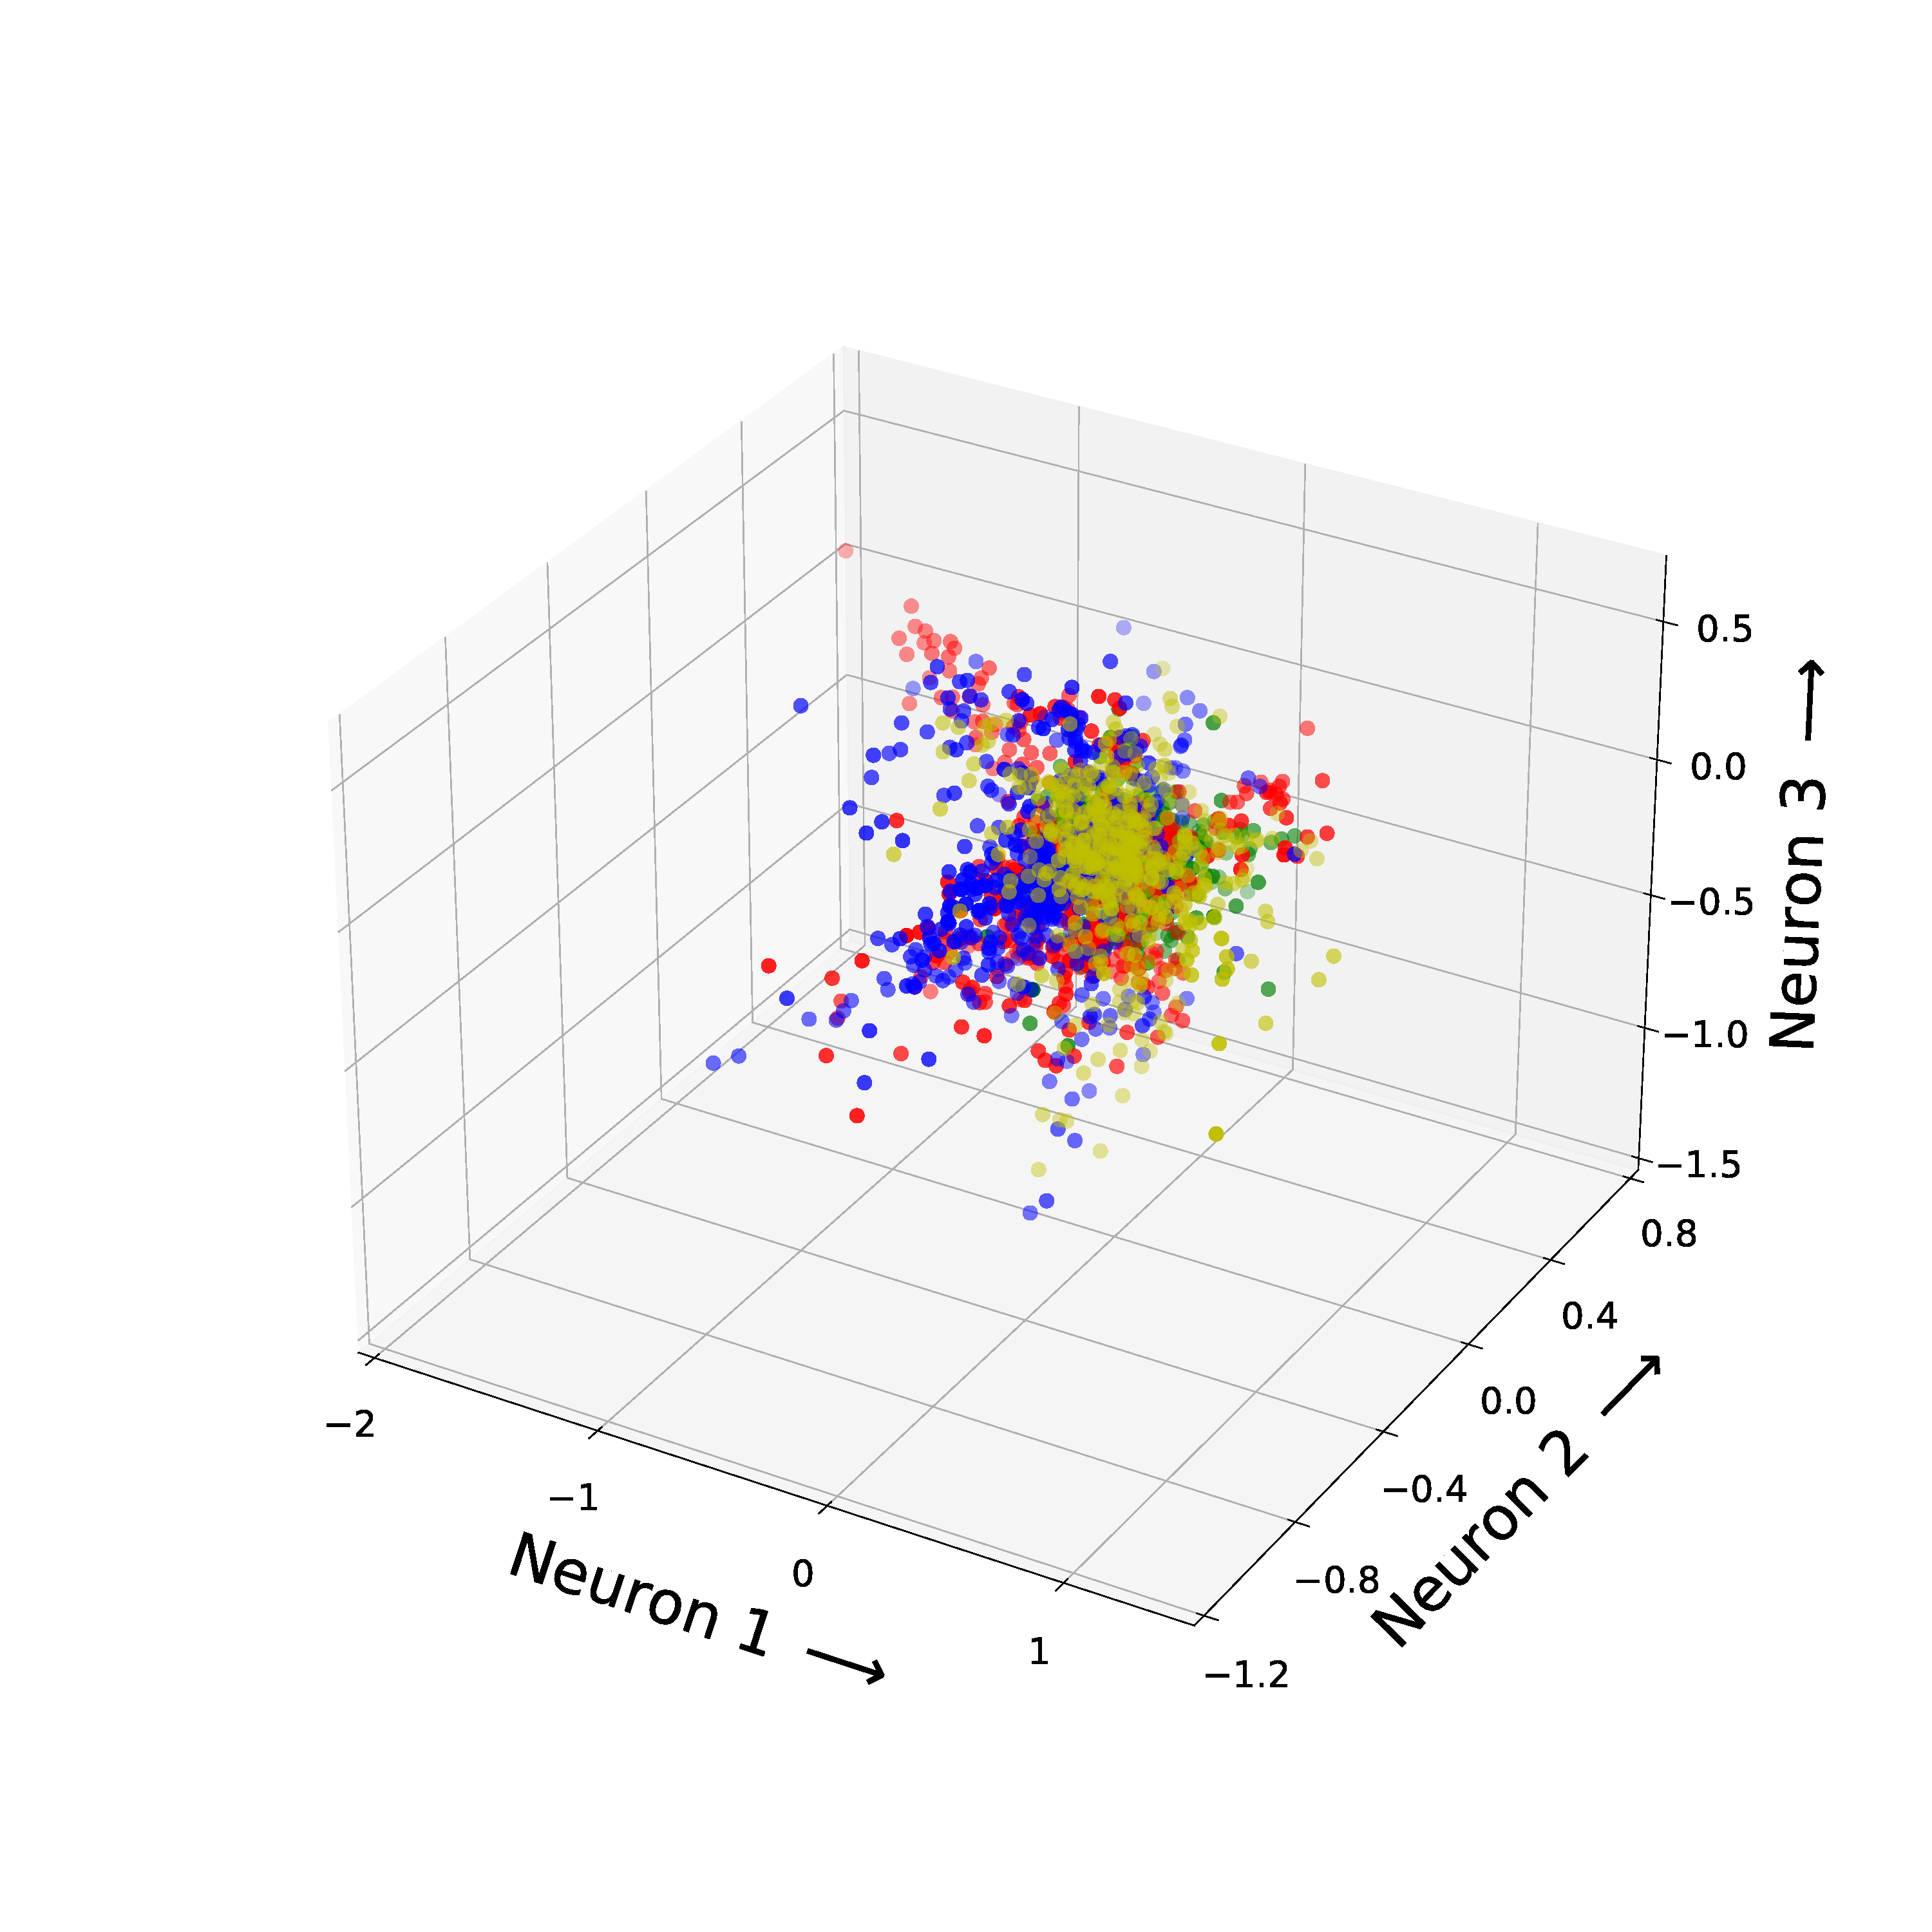
\includegraphics[width=.48\textwidth]{GAMMA_Influence_dummy_distribution/Dummy_distribution_0_GAMMA_0_001.pdf}
  \hspace{.4cm}
  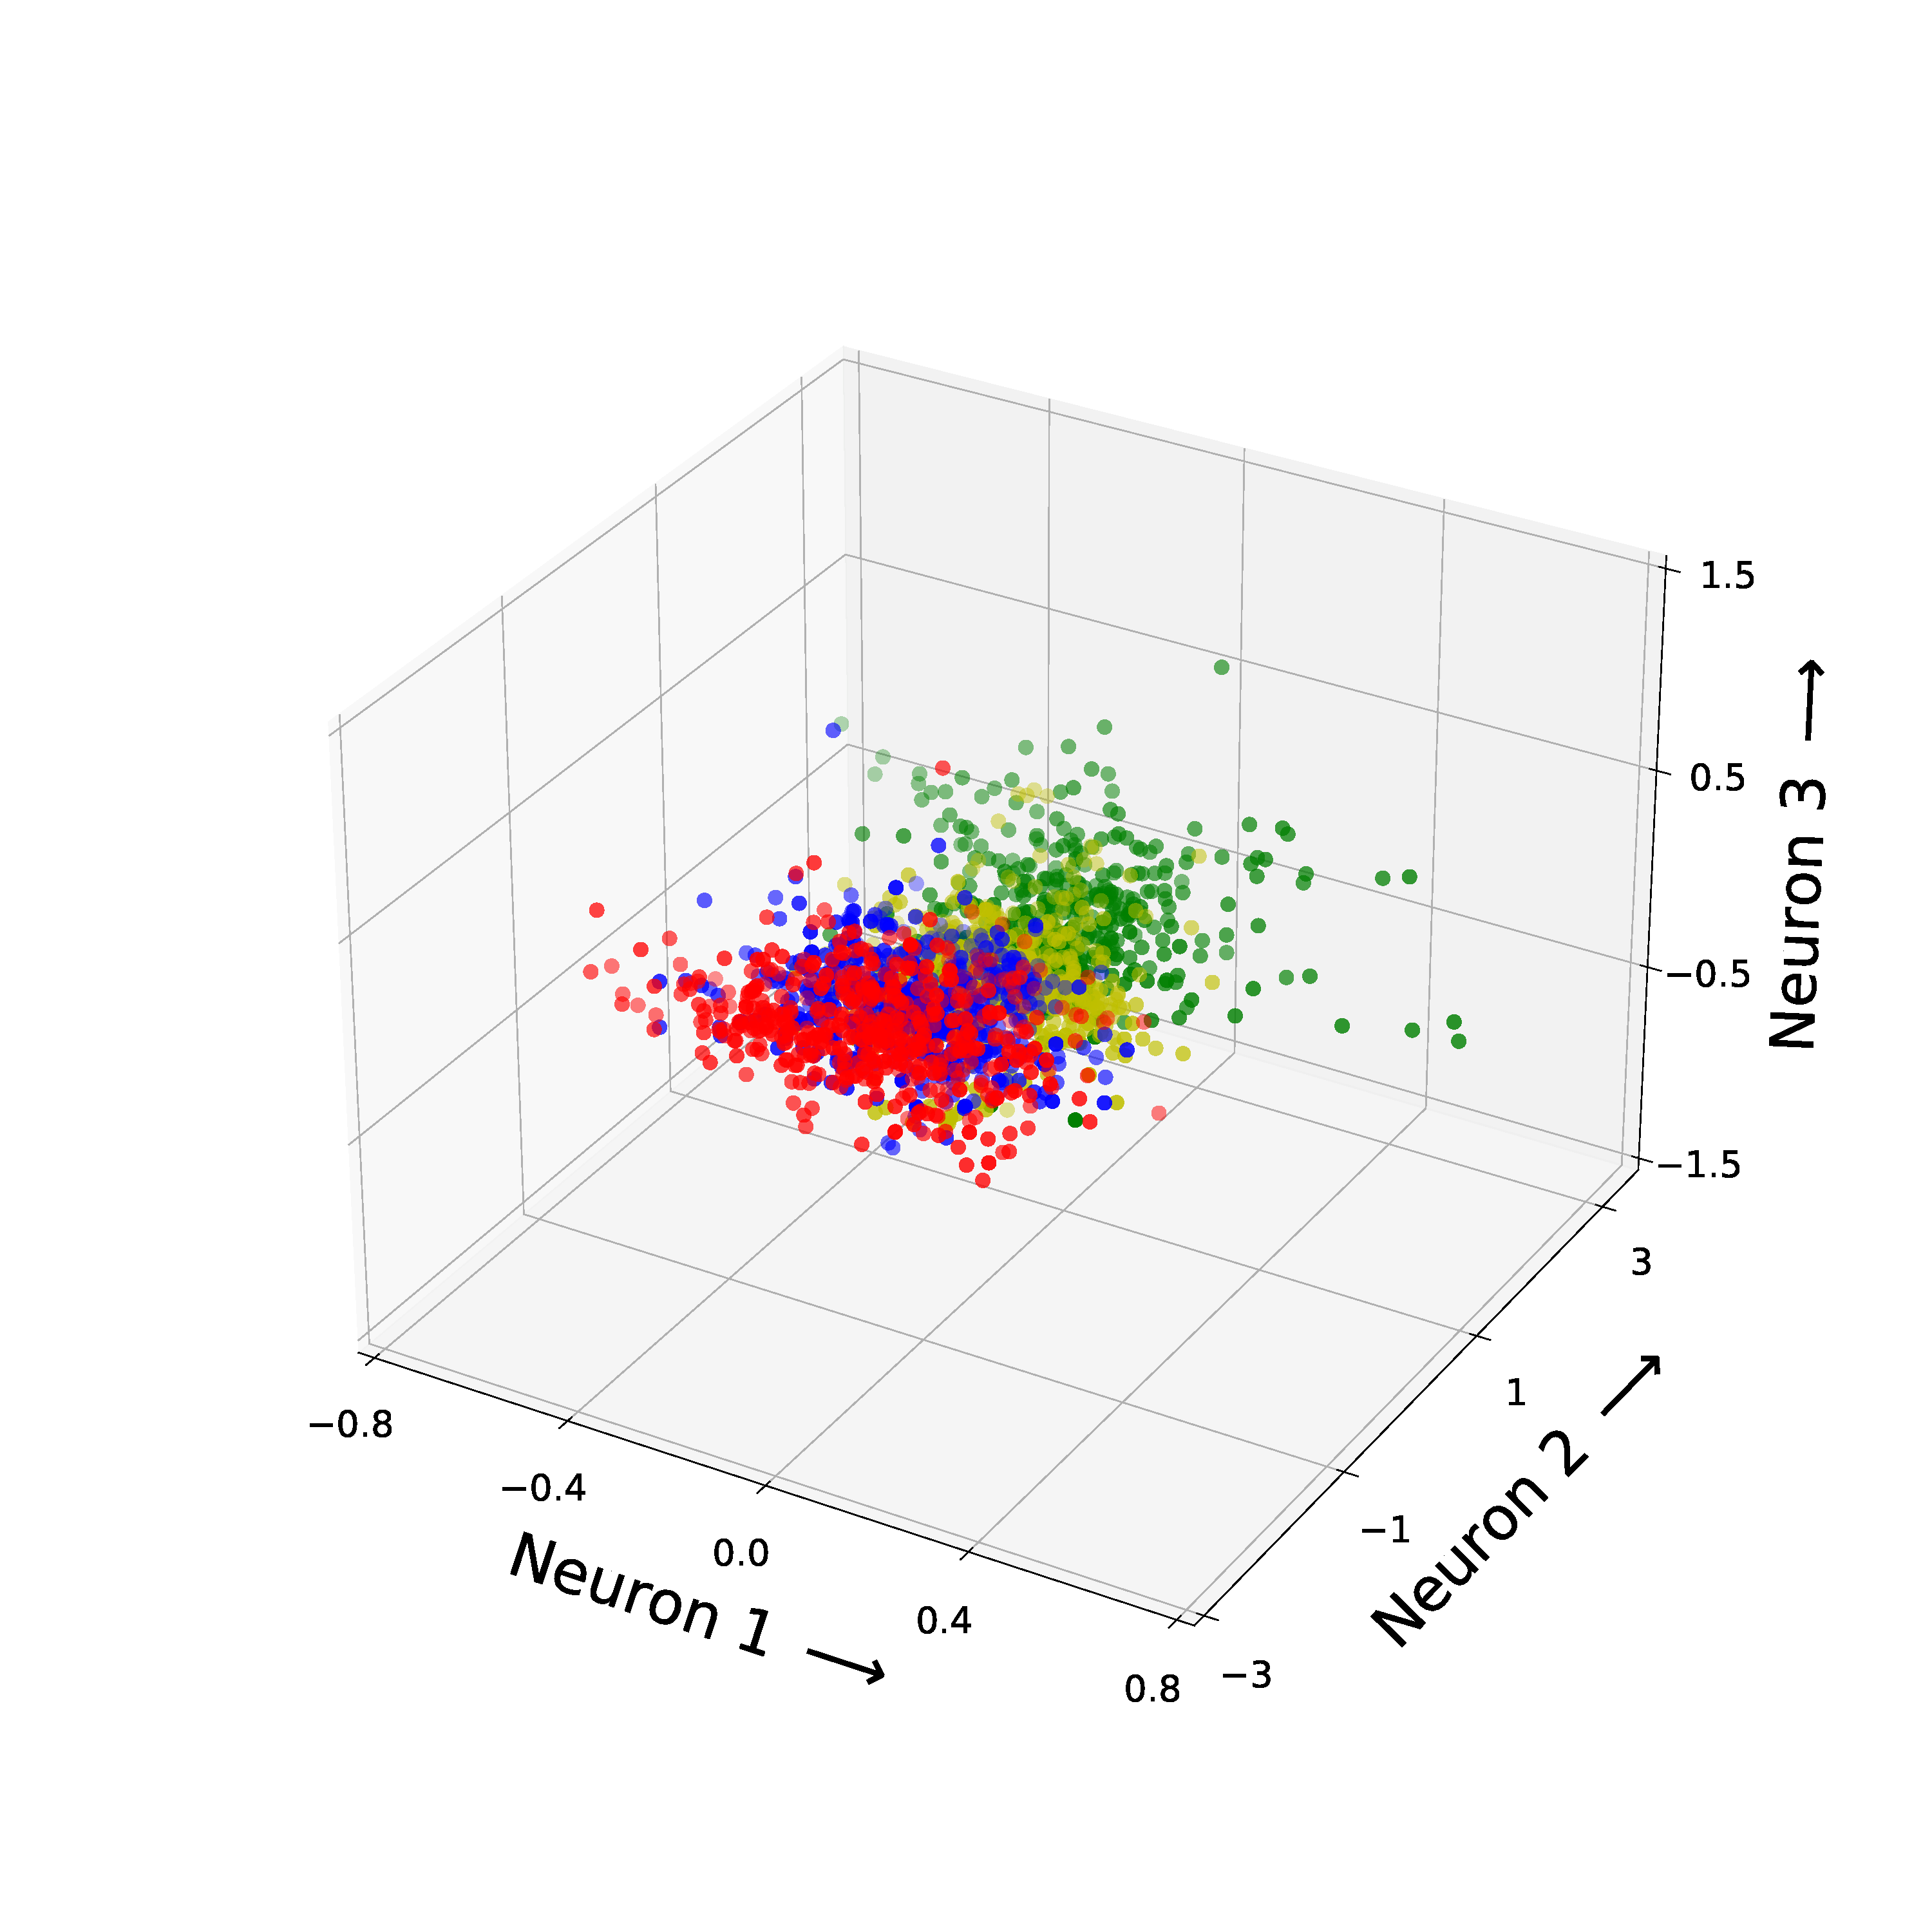
\includegraphics[width=.48\textwidth]{GAMMA_Influence_dummy_distribution/Dummy_distribution_8_GAMMA_0_001.pdf}

  \vspace{.1cm}

  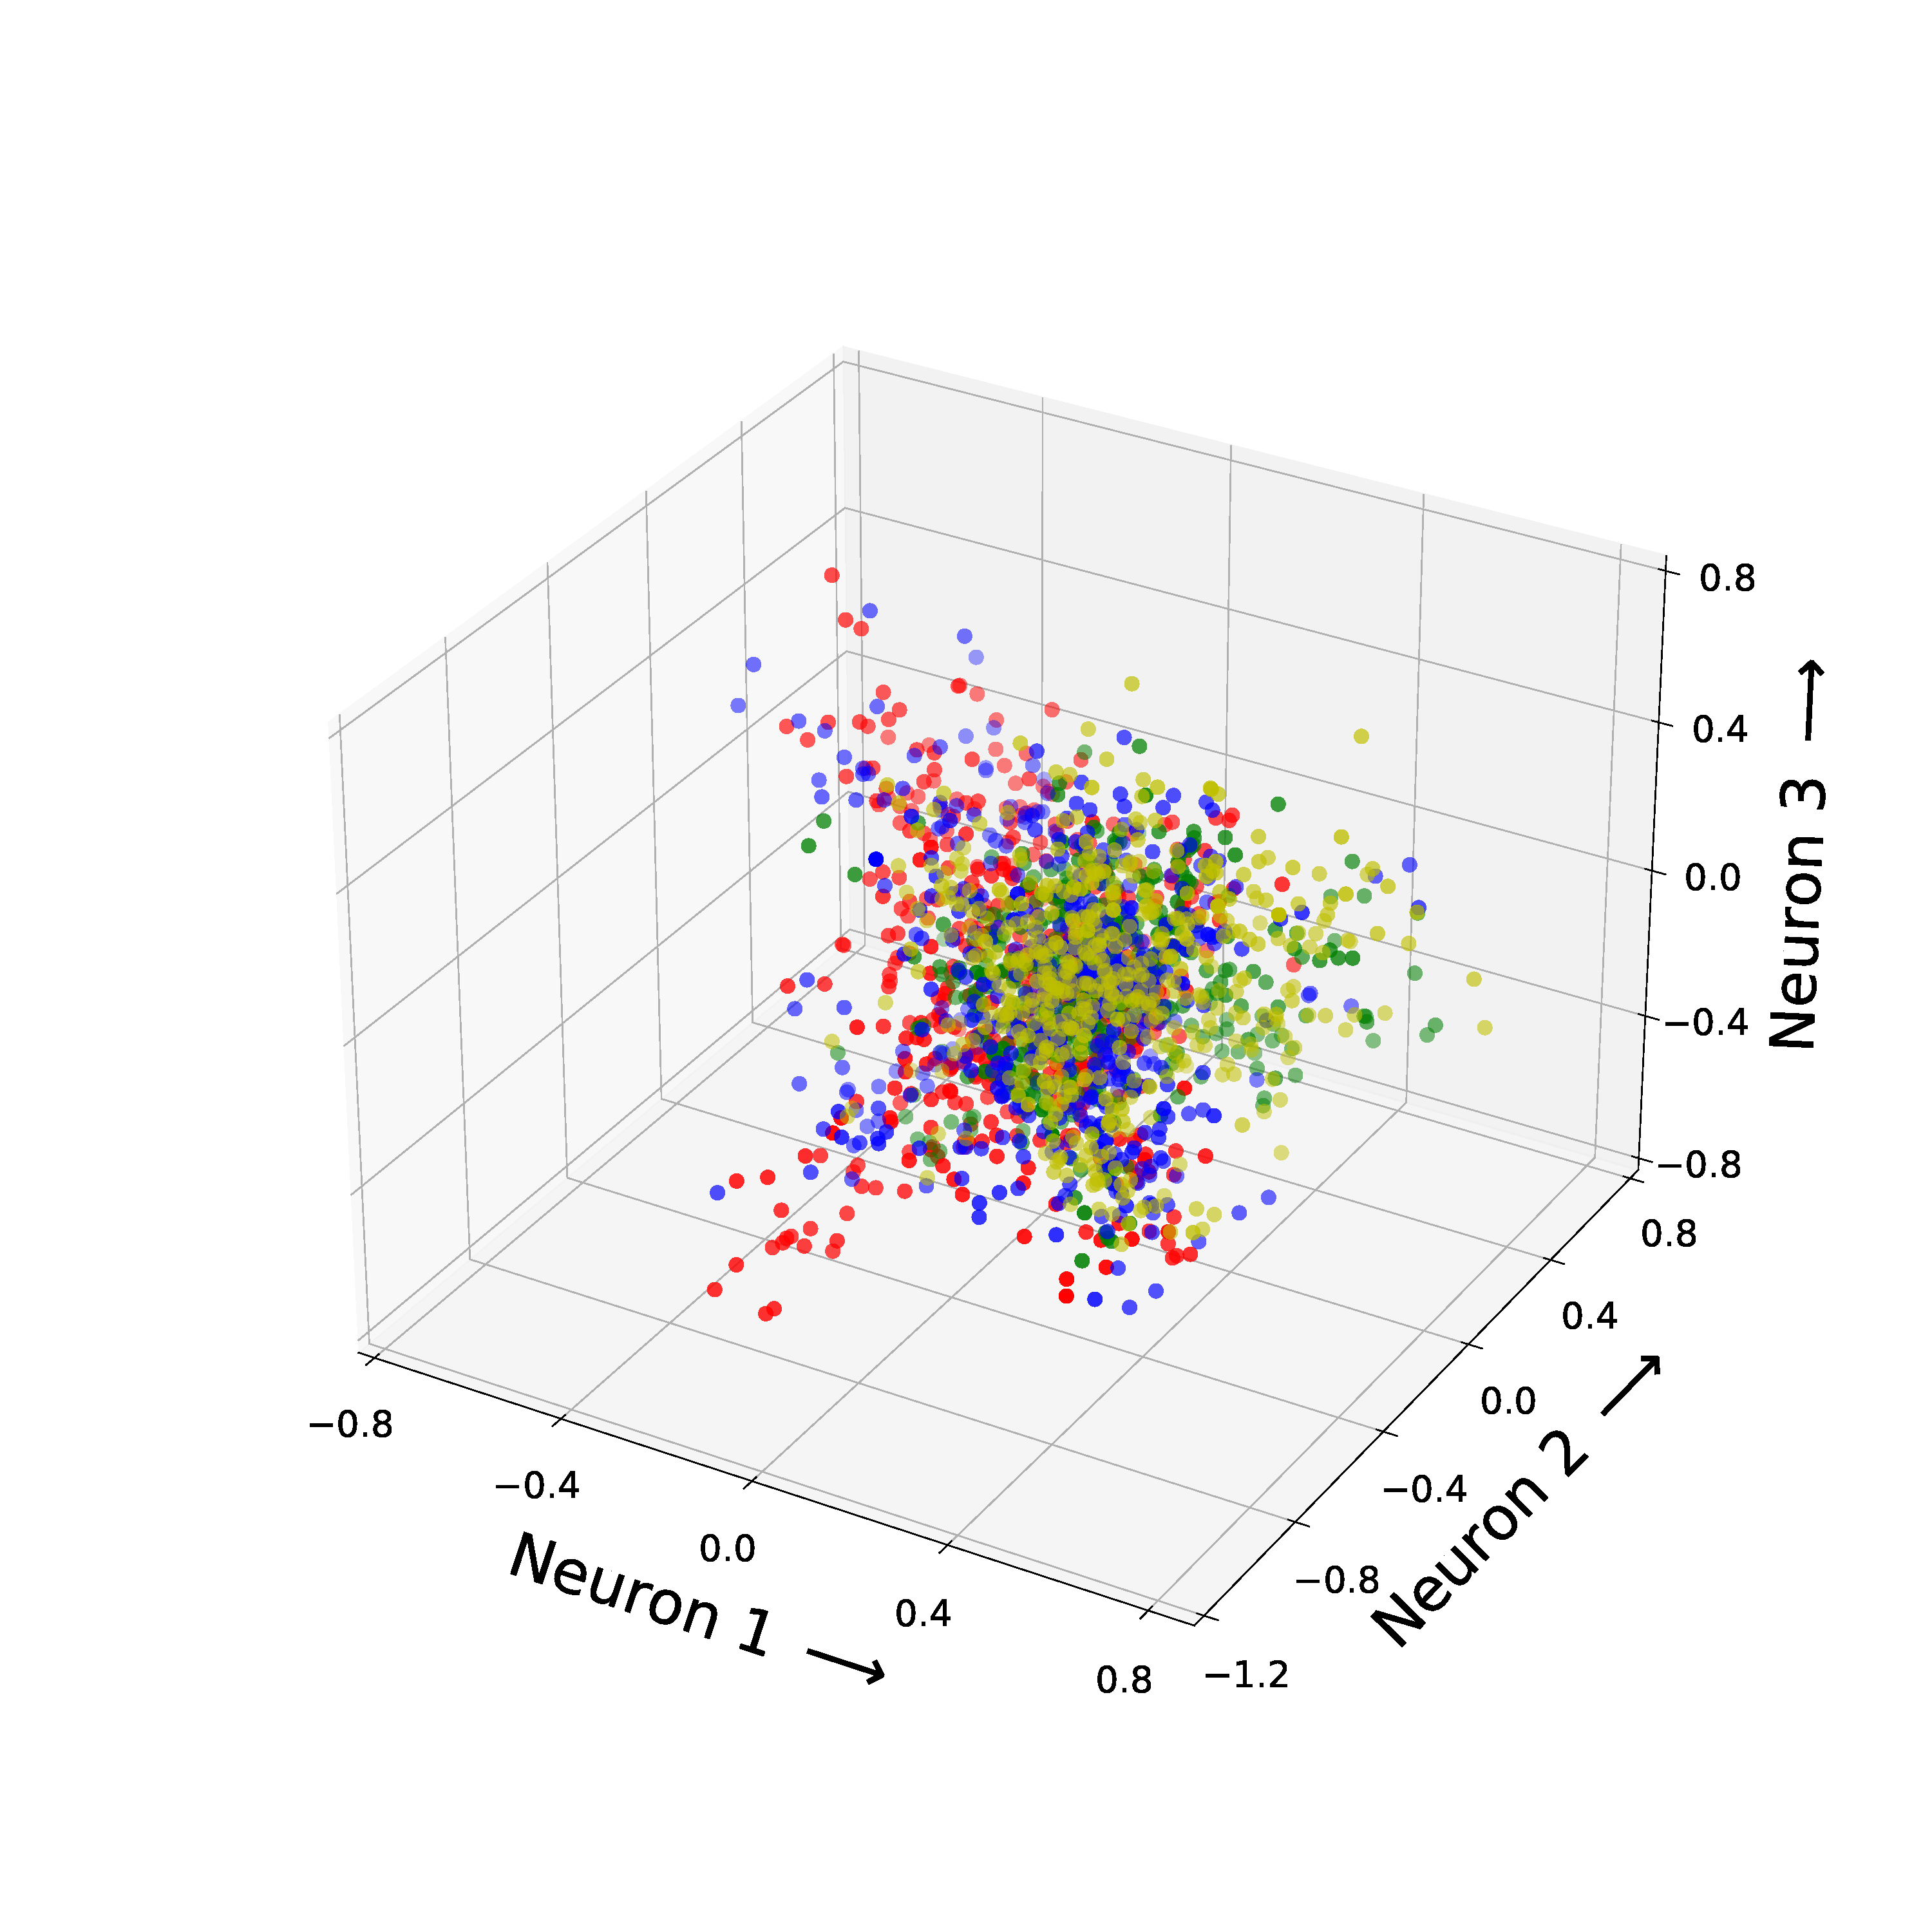
\includegraphics[width=.48\textwidth]{GAMMA_Influence_dummy_distribution/Dummy_distribution_0_GAMMA_0_1.pdf}
  \hspace{.4cm}
  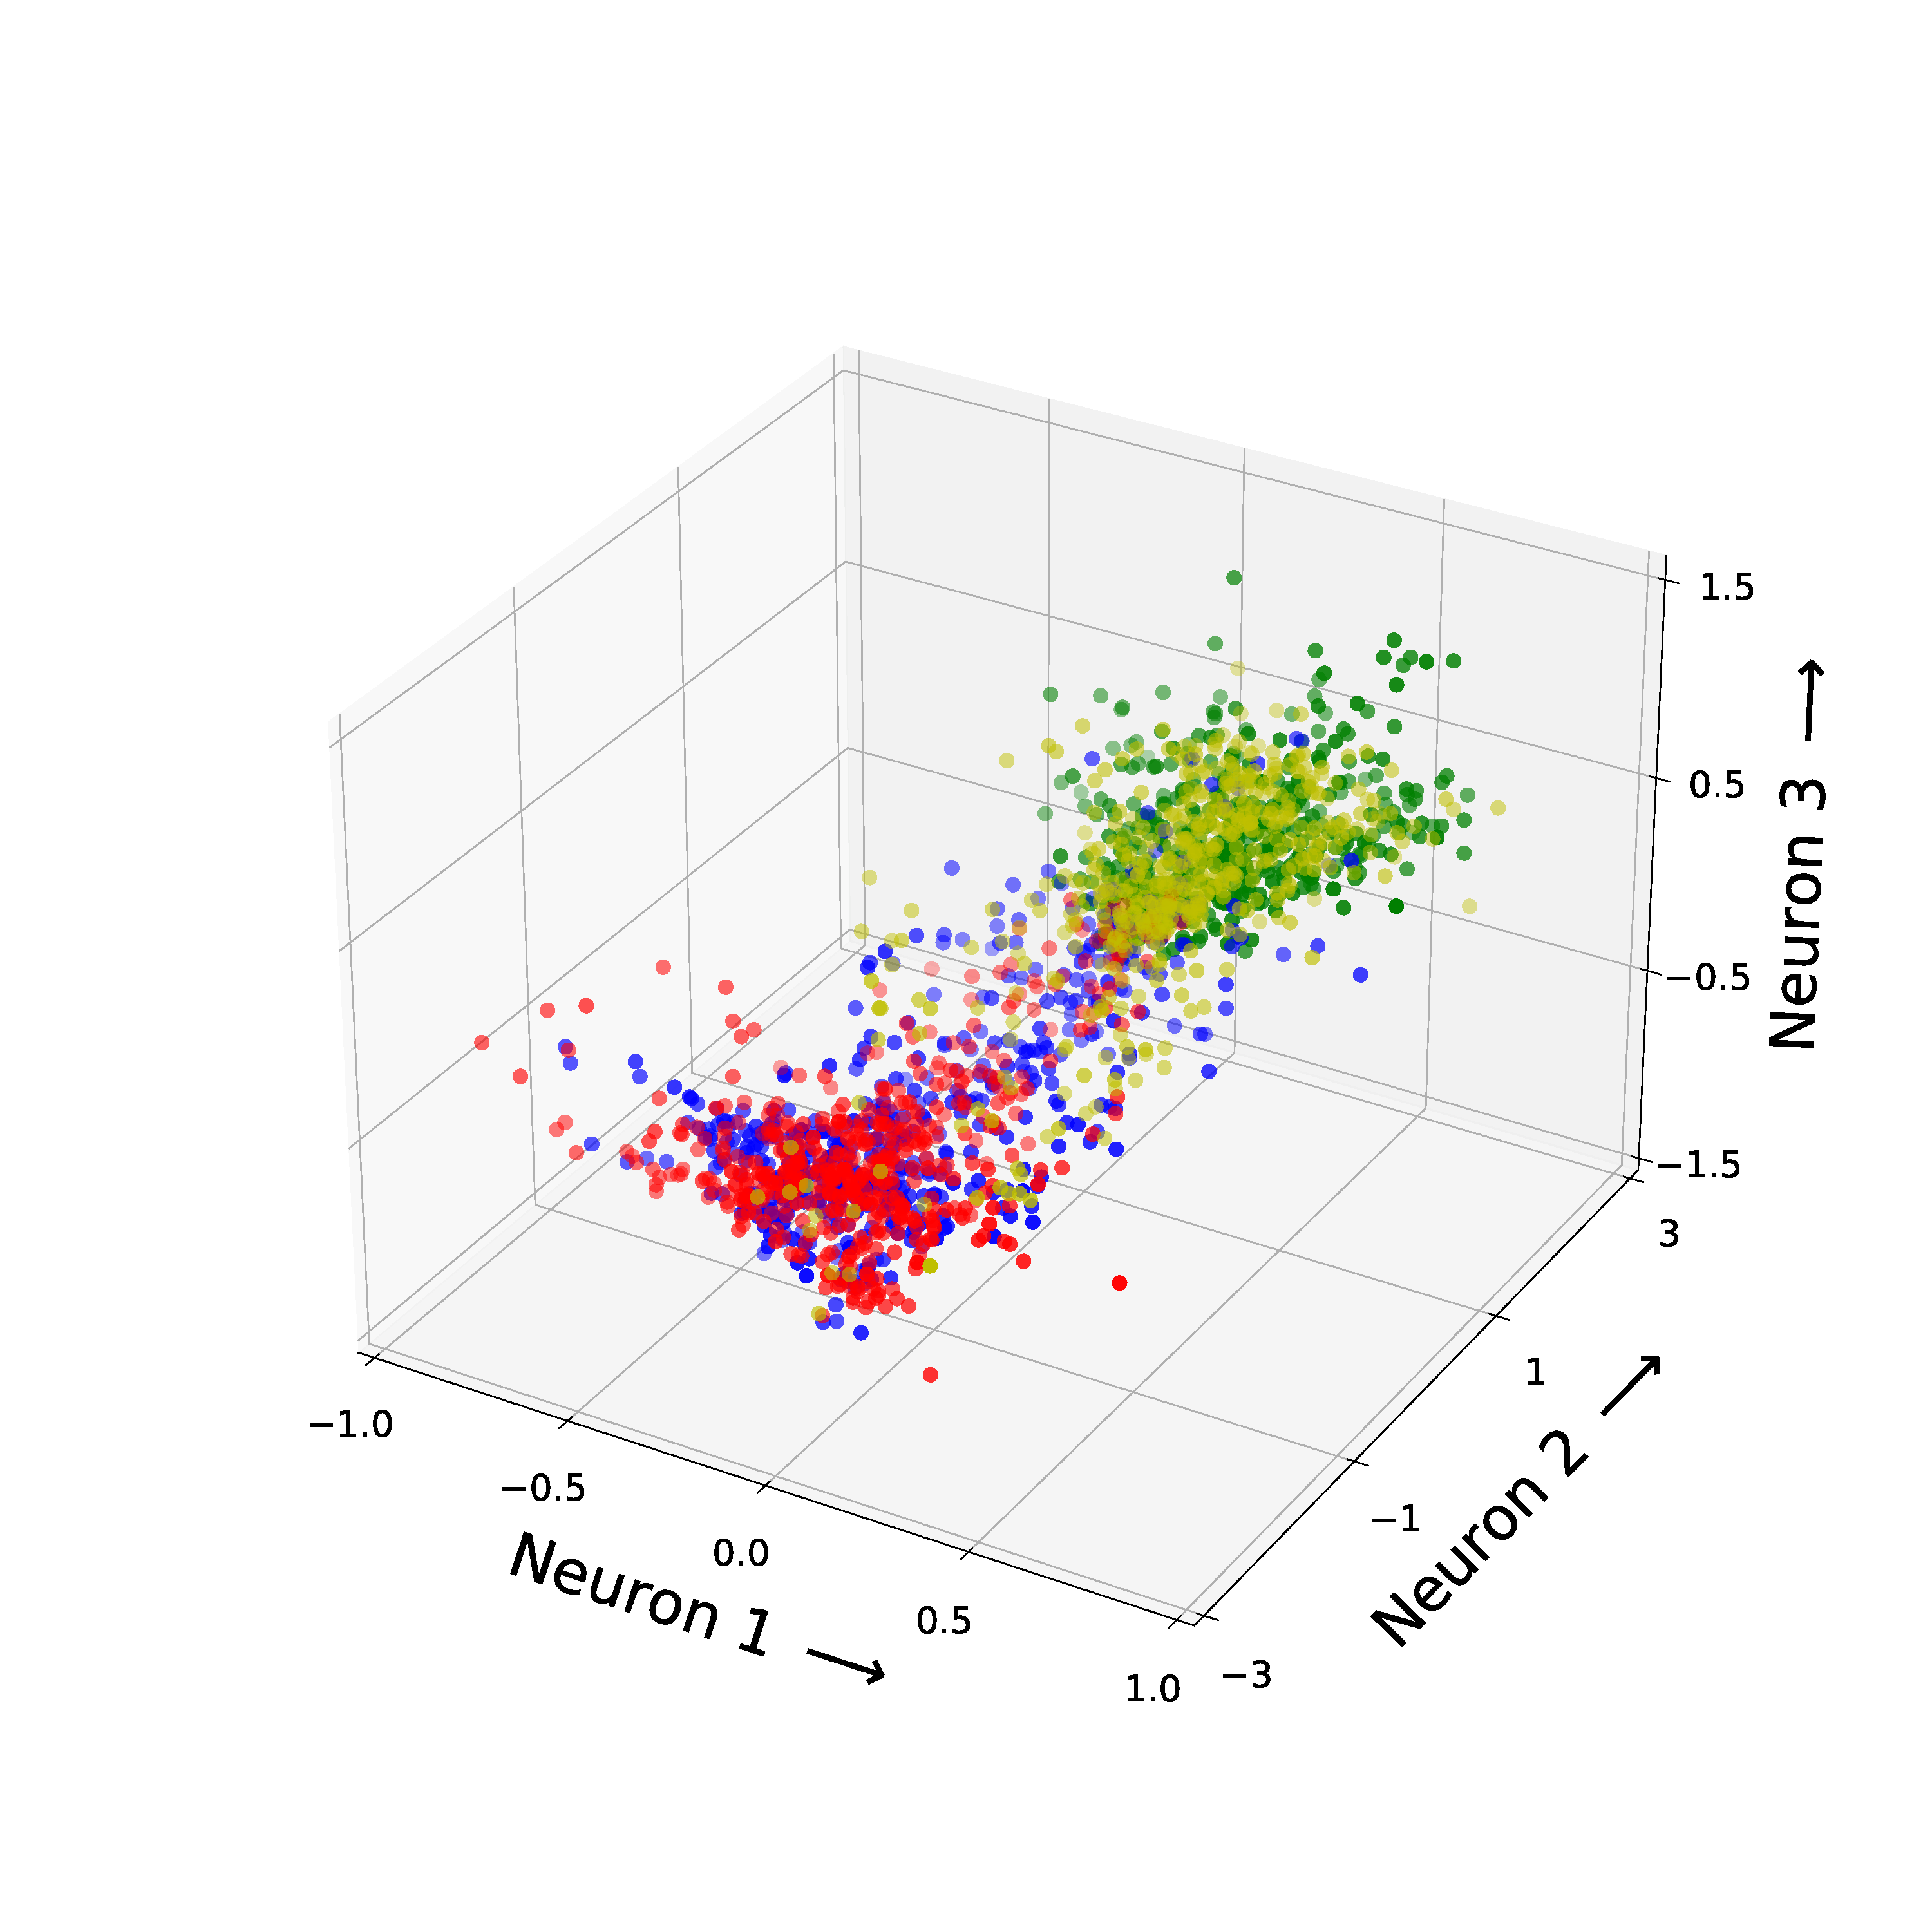
\includegraphics[width=.48\textwidth]{GAMMA_Influence_dummy_distribution/Dummy_distribution_8_GAMMA_0_1.pdf}

  \vspace{.1cm}

  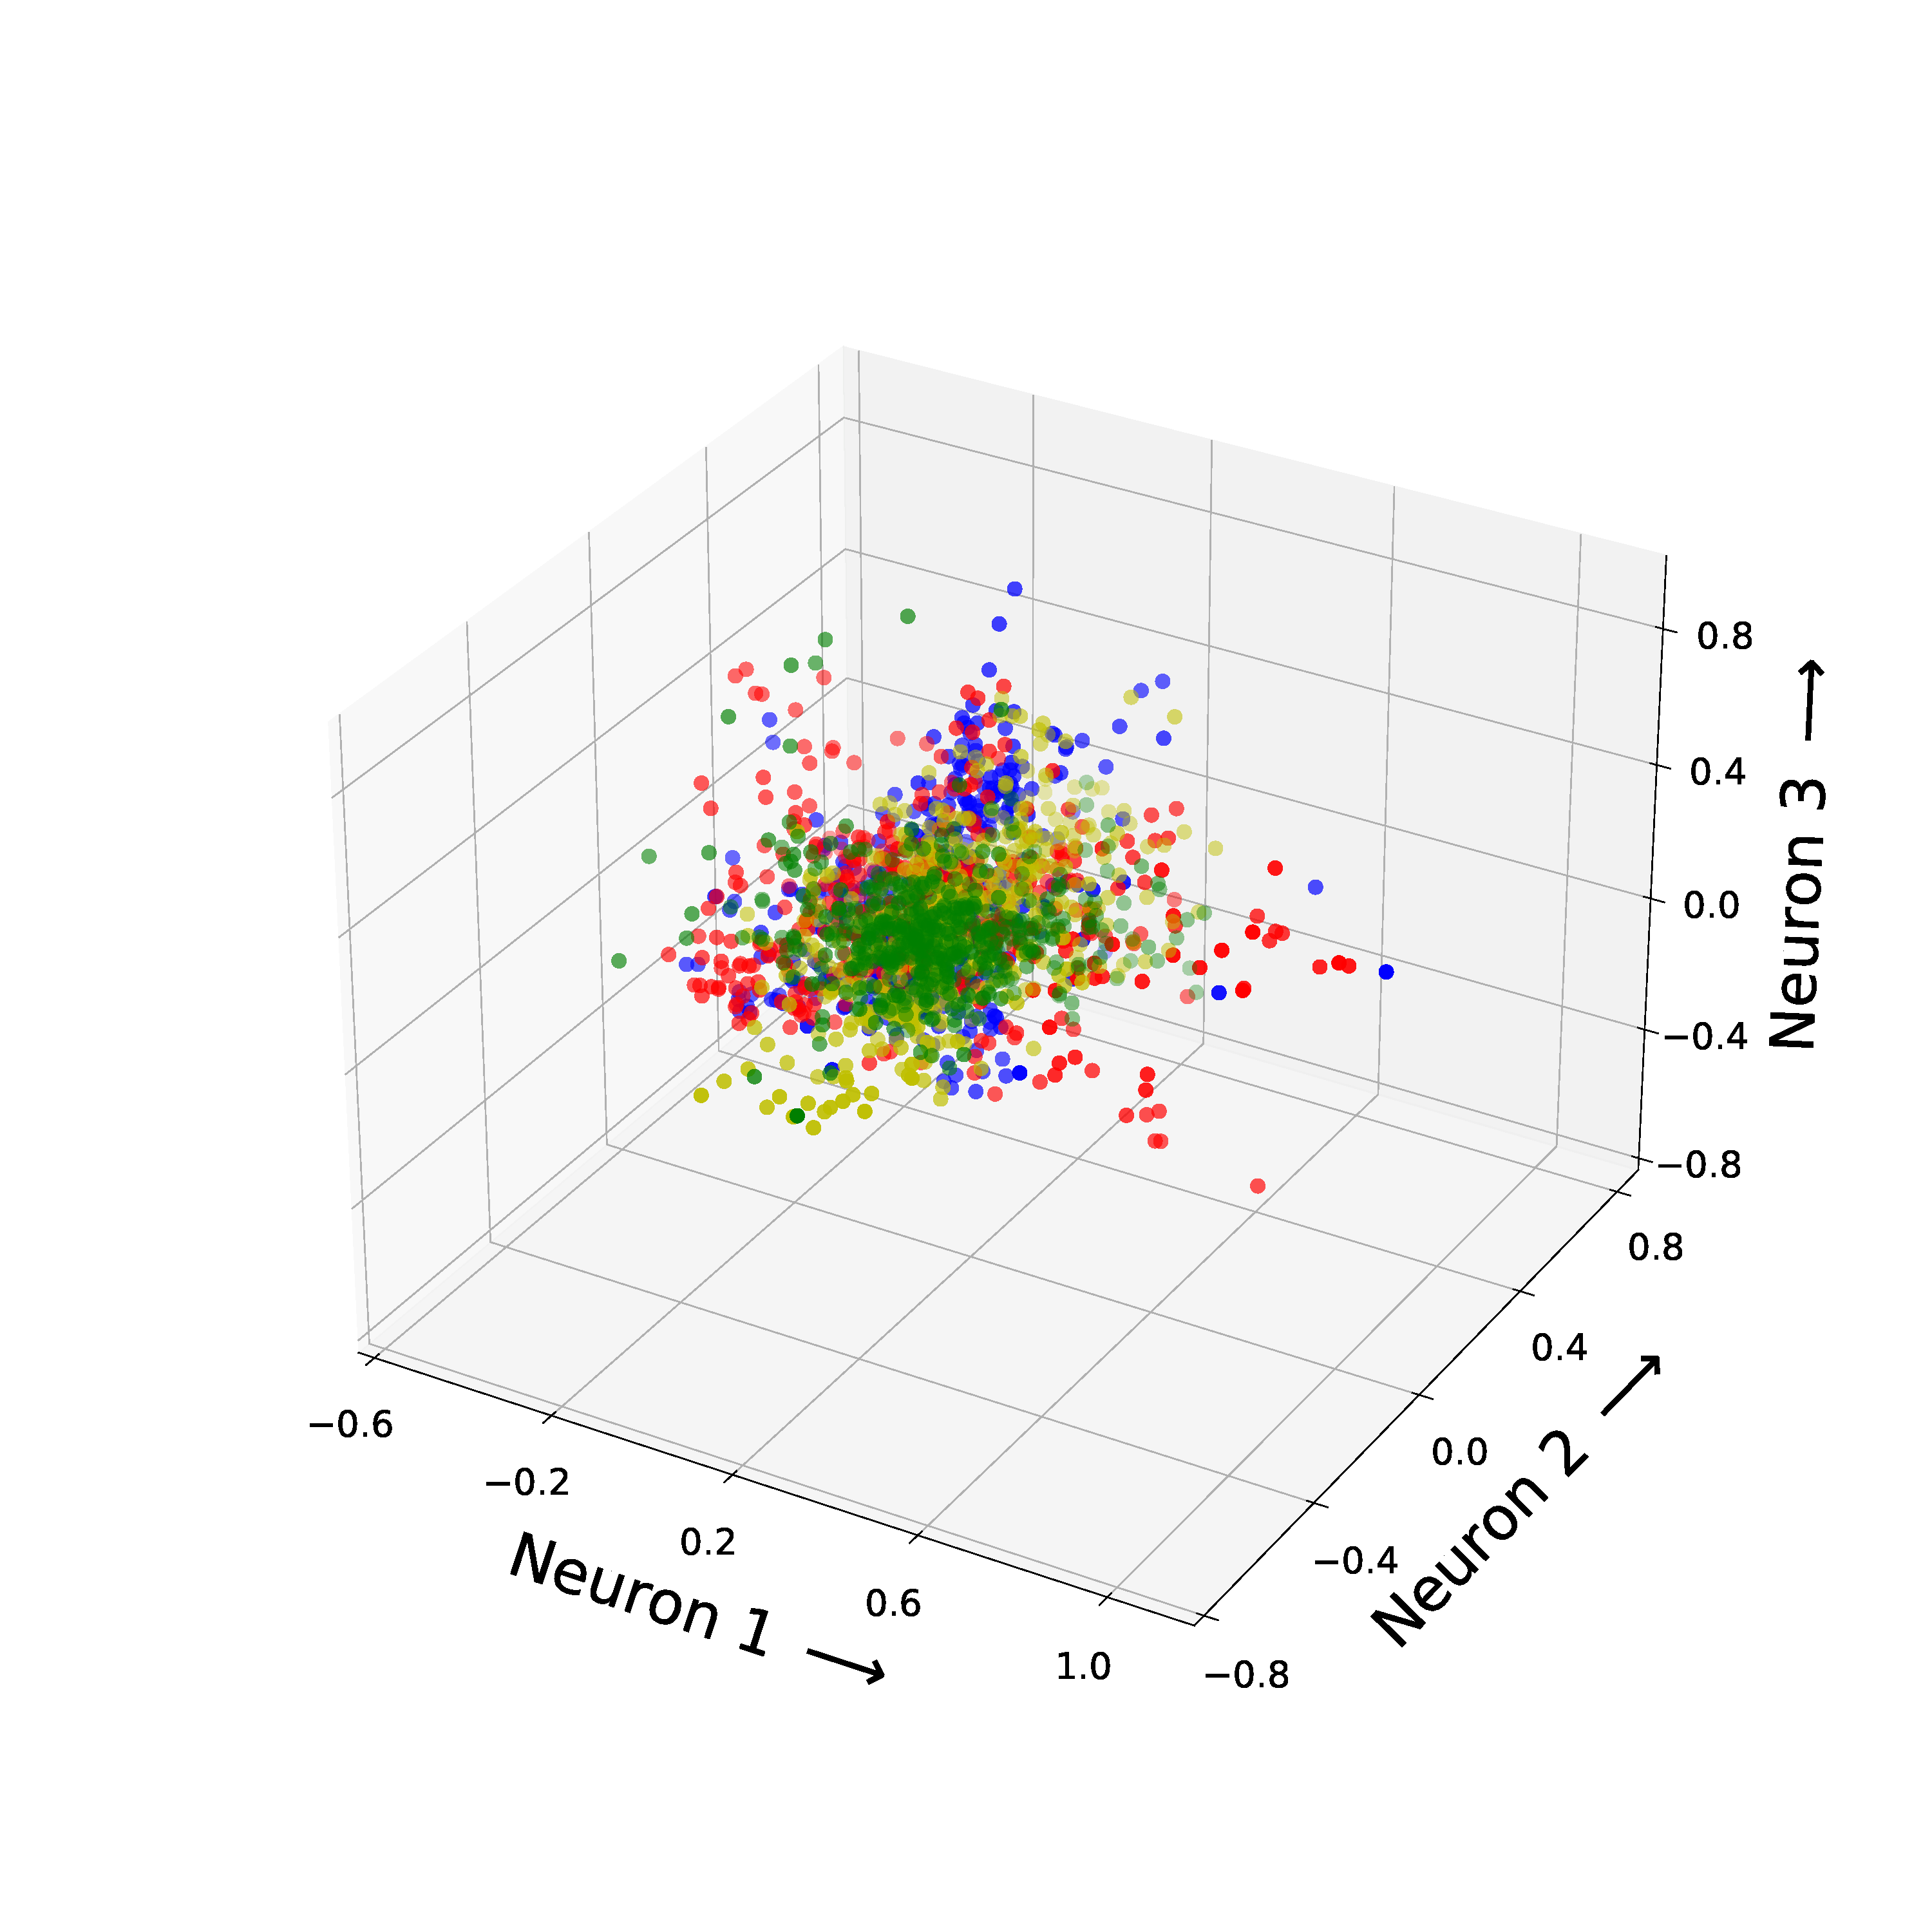
\includegraphics[width=.48\textwidth]{GAMMA_Influence_dummy_distribution/Dummy_distribution_0_GAMMA_20.pdf}
  \hspace{.4cm}
  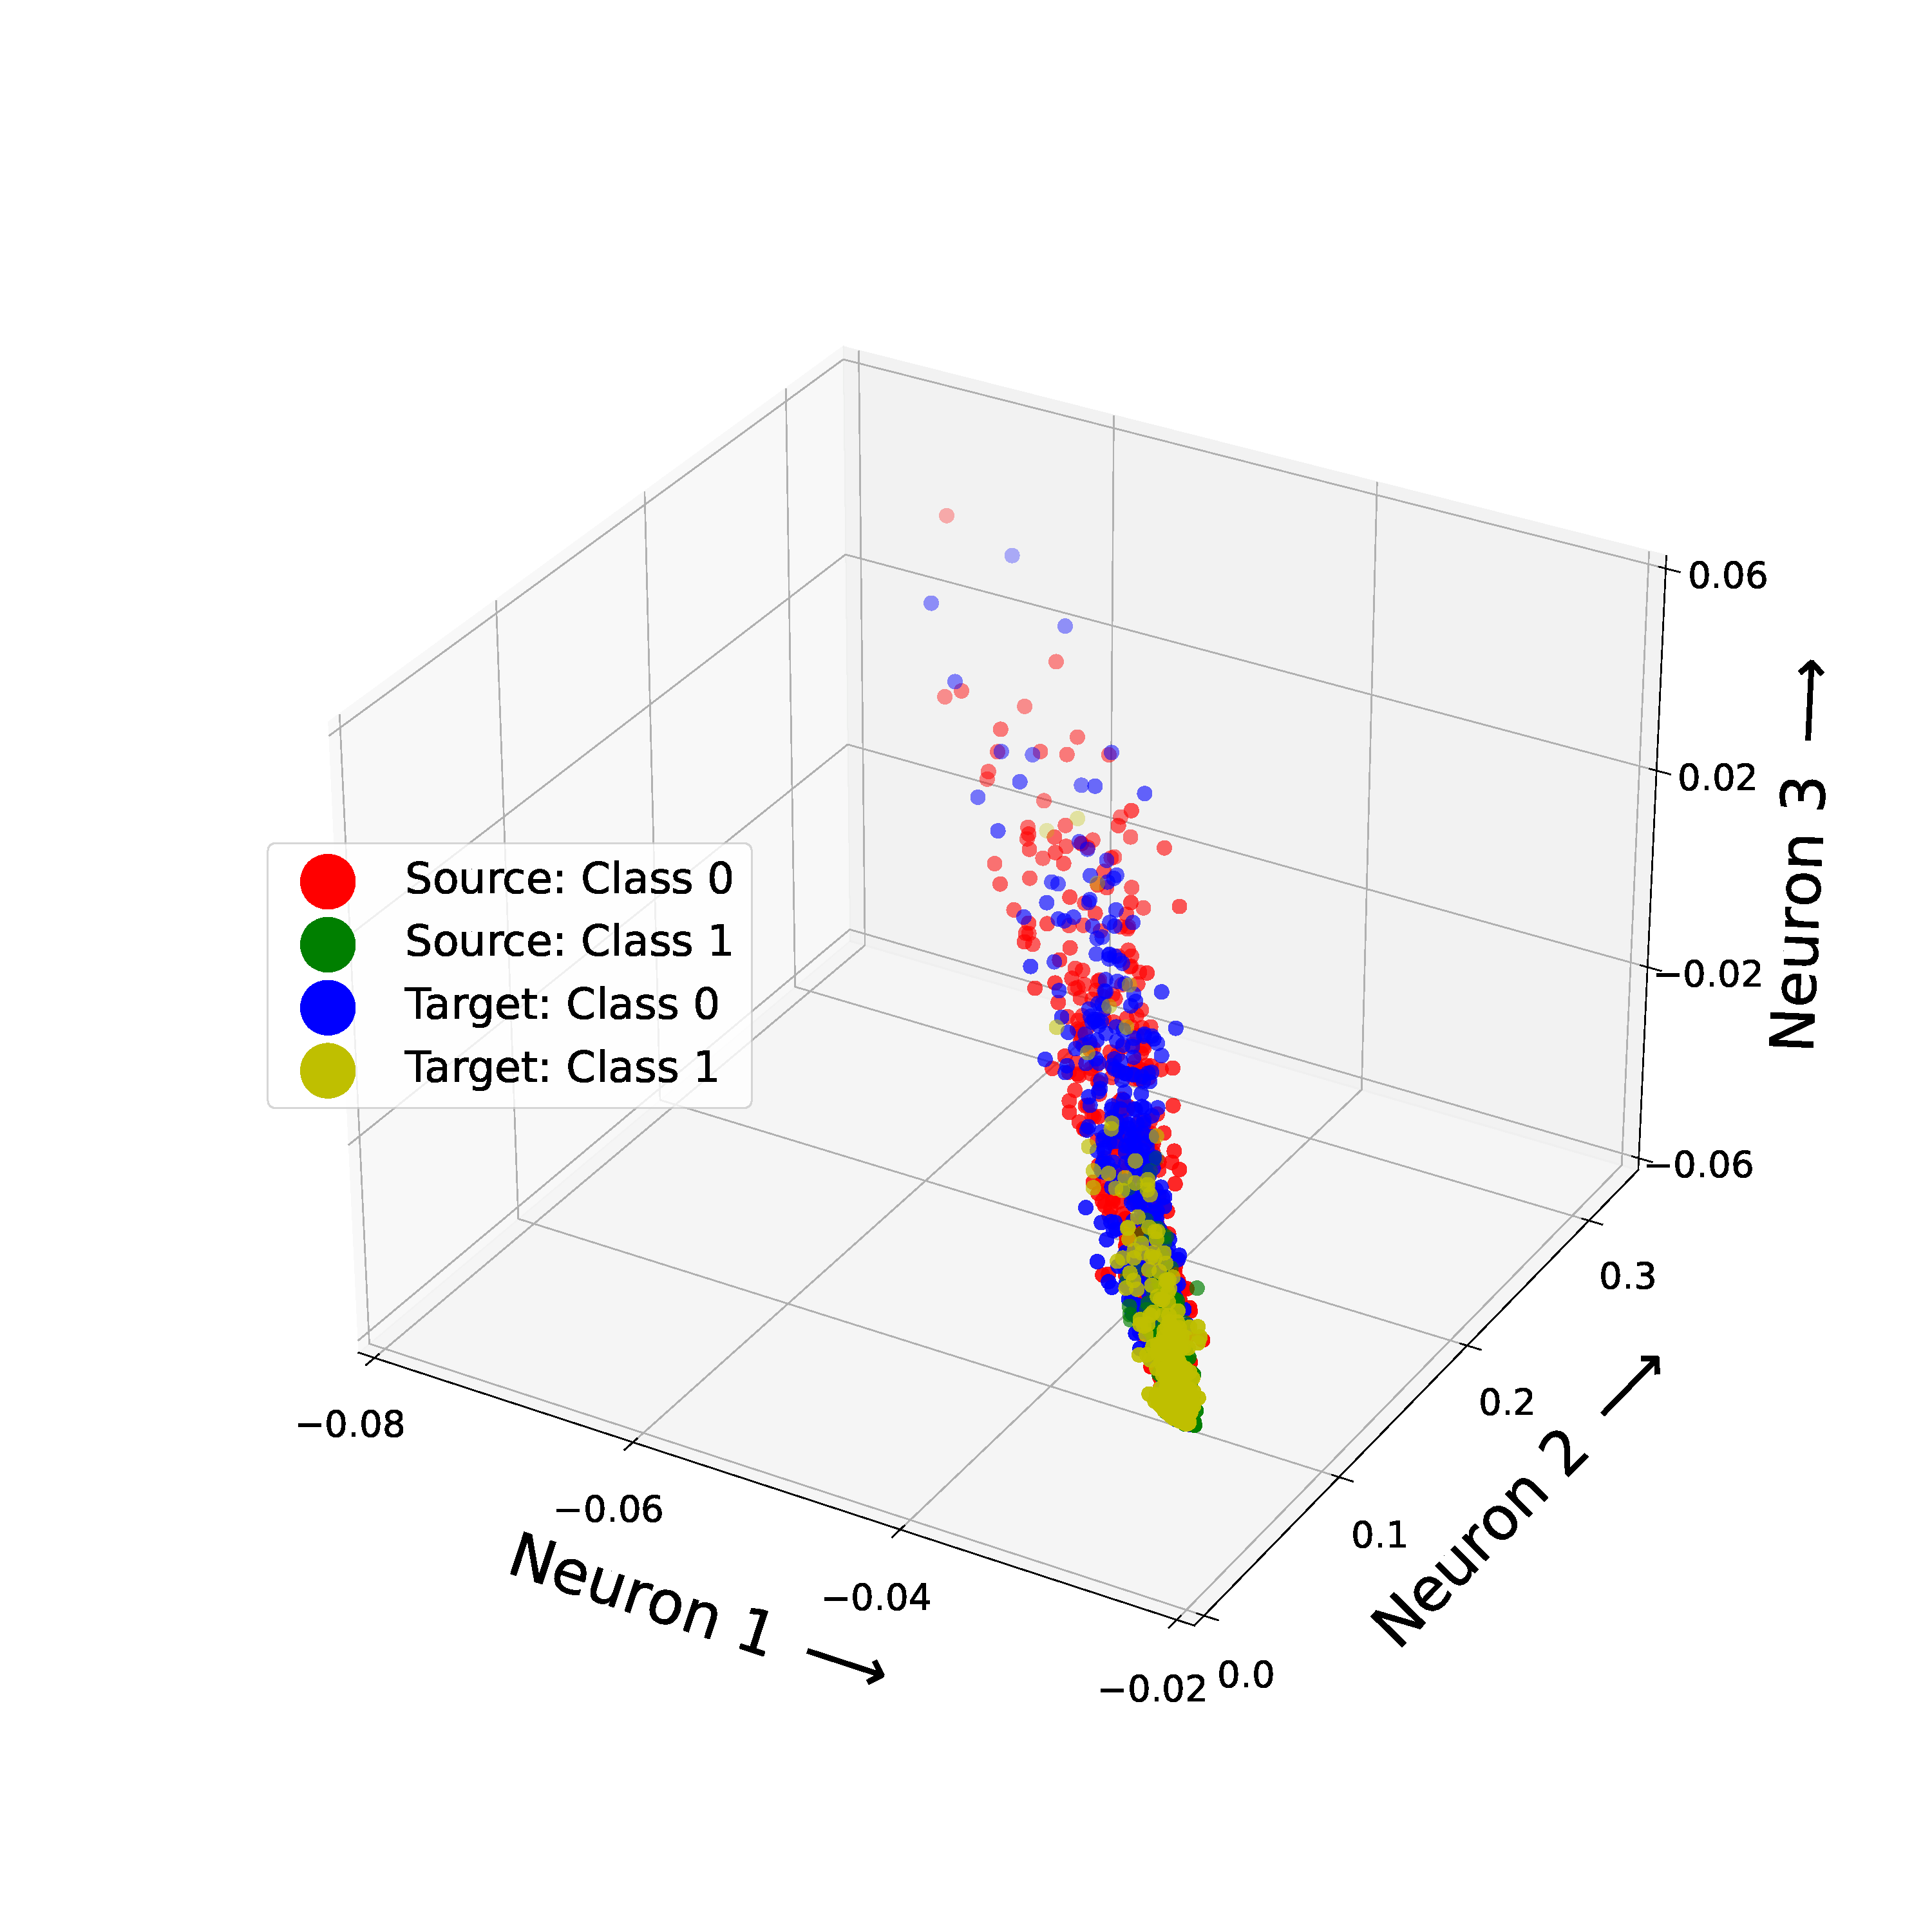
\includegraphics[width=.48\textwidth]{GAMMA_Influence_dummy_distribution/Dummy_distribution_8_GAMMA_20.pdf}
 

  \caption{Data distribution: Influence of GAMMA on Training, GAMMA = 0.05 (top), GAMMA = 0,4 (middle), GAMMA = 20 (bottom), Epoch = 0 (left) , Epoch = 8 (right)}
  \label{fig:point_cloud_mmd}
\end{figure}


\begin{figure}[htp]
  \centering
  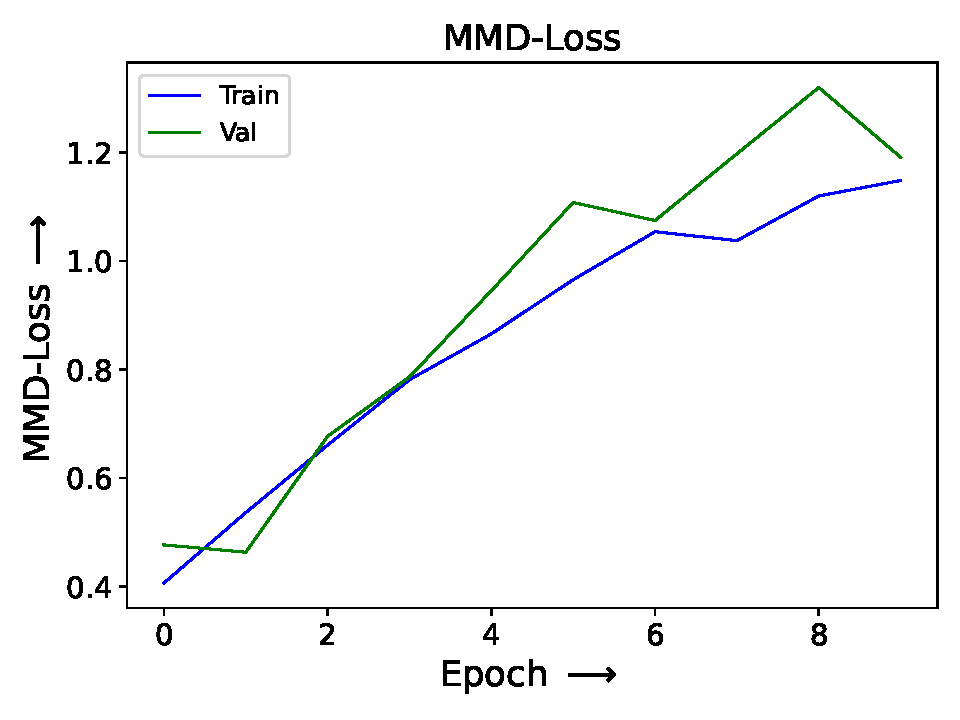
\includegraphics[width=.47\textwidth]{GAMMA_Influence_dummy_curve/MMD_Loss_GAMMA_0_001.pdf}
  \hspace{.3cm}
  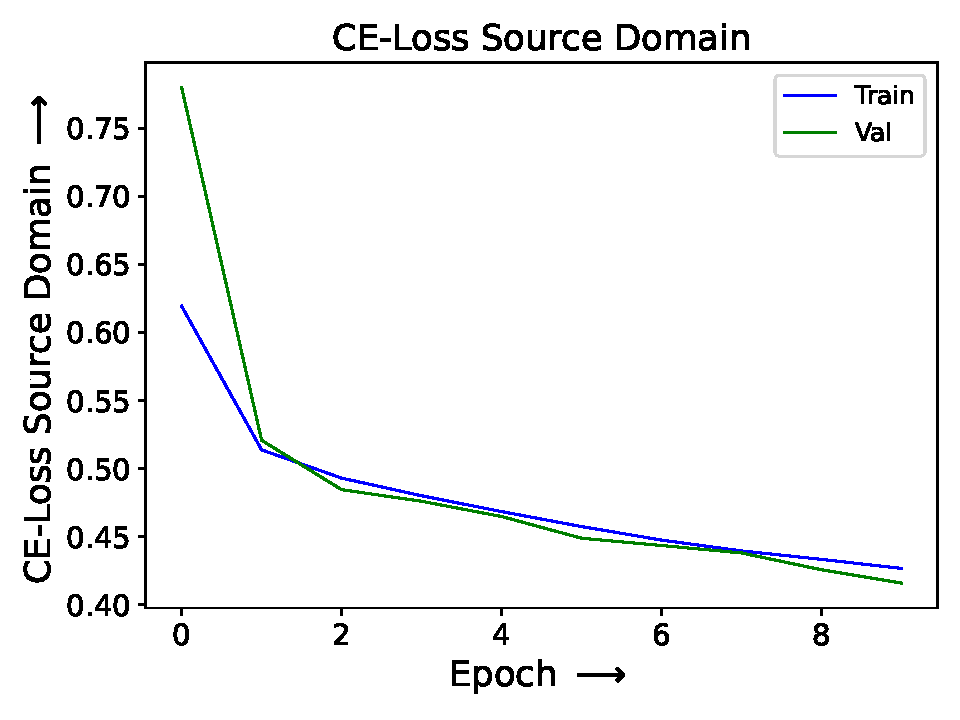
\includegraphics[width=.47\textwidth]{GAMMA_Influence_dummy_curve/CE_Loss_Source_Domain_GAMMA_0_001.pdf}

  \vspace{.1cm}

  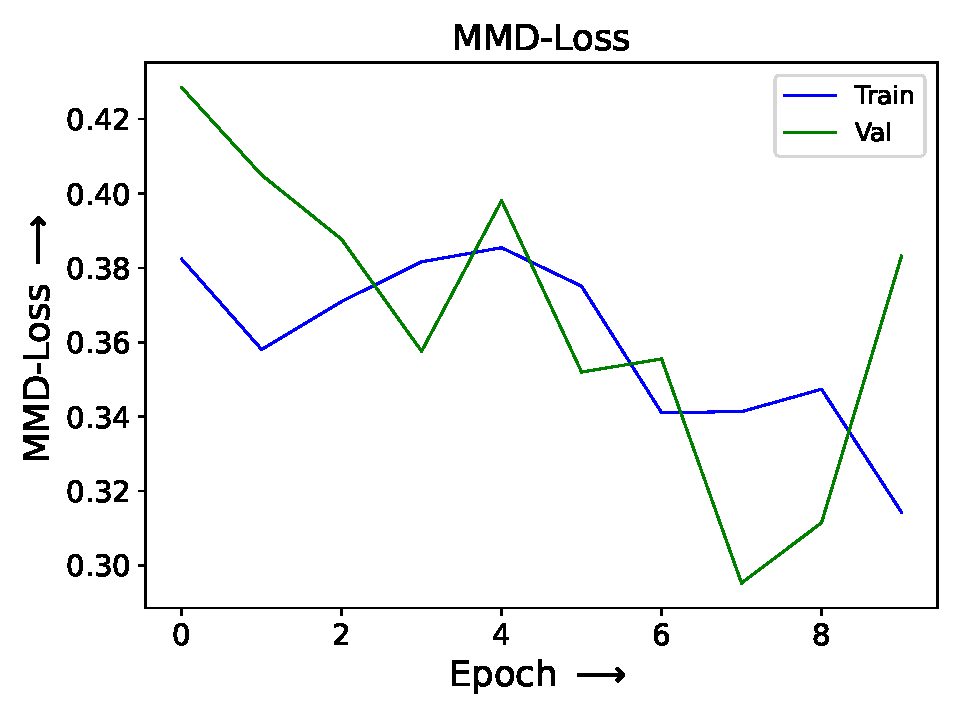
\includegraphics[width=.47\textwidth]{GAMMA_Influence_dummy_curve/MMD_Loss_GAMMA_0_1.pdf}
  \hspace{.3cm}
  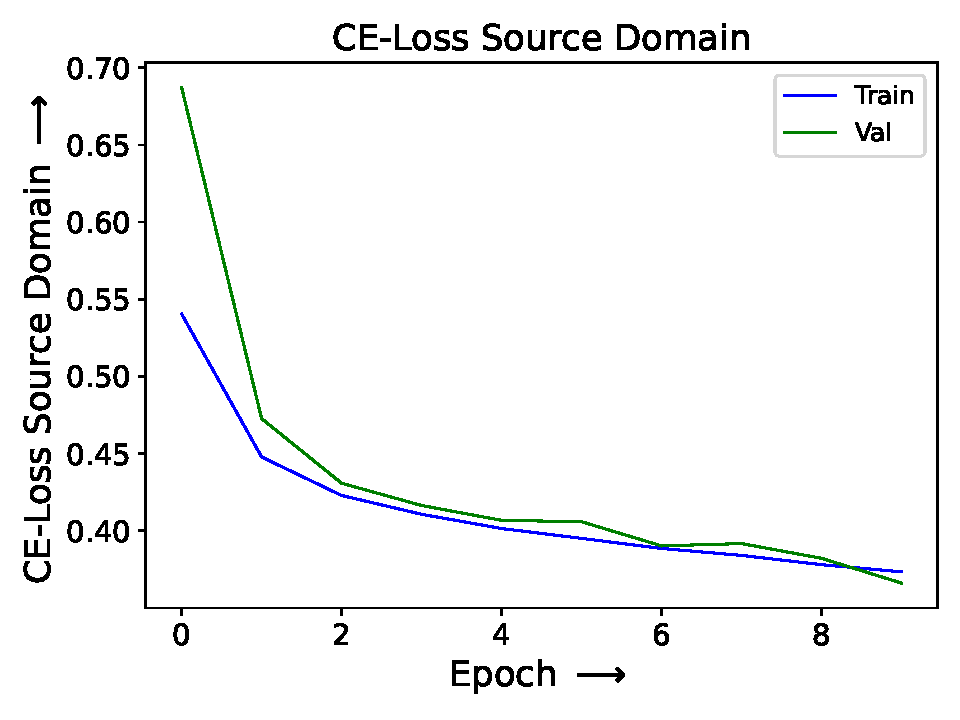
\includegraphics[width=.47\textwidth]{GAMMA_Influence_dummy_curve/CE_Loss_Source_Domain_GAMMA_0_1.pdf}

  \vspace{.1cm}

  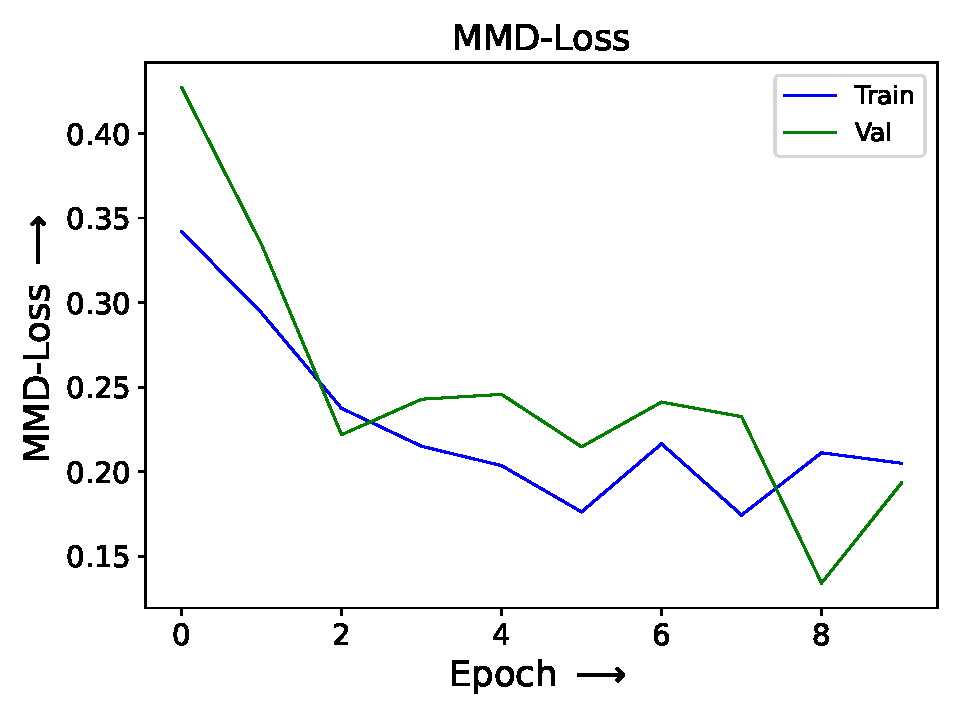
\includegraphics[width=.47\textwidth]{GAMMA_Influence_dummy_curve/MMD_Loss_GAMMA_20.pdf}
  \hspace{.1cm}
  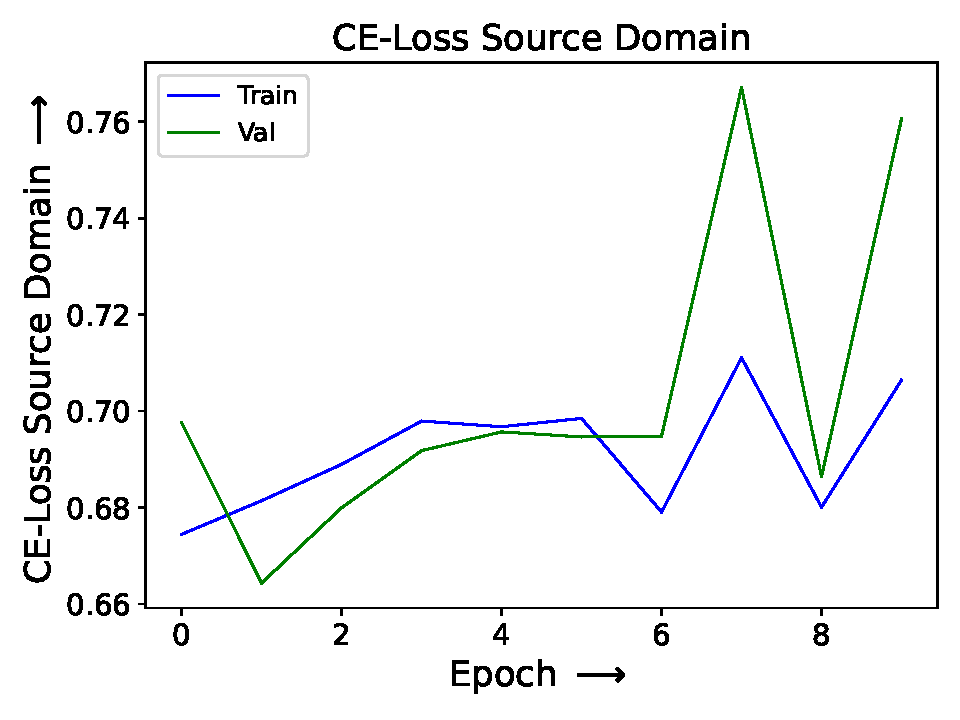
\includegraphics[width=.47\textwidth]{GAMMA_Influence_dummy_curve/CE_Loss_Source_Domain_GAMMA_20.pdf}

  \caption{MMD- and source CE-loss: Influence of GAMMA on Training: GAMMA = 0.001 (top), GAMMA = 0.1 (middle), GAMMA = 20 (bottom), Epoch 0 (left), Epoch 8 (right)}
  \label{fig:learning_curves_influence_mmd_feature_extractor}
\end{figure}

\subsection{Domain Adaption Performance of a Labeled MMD-loss} \label{sec:Differences of labeled and unlabeled MMD loss}

The idea behind domain adaption is to aggregate knowledge while solving one problem and transferring that knowledge to another problem. For this reason, in domain adaption tasks the goal is to restrict the supervised learning solely on the source domain data. In the regular MMD-loss, the target labels are unknown. Therefore, the intra- and inter-class distance between source and target samples is minimized equally. Obviously, this reduces the class separability in both domains. In the literature, domain adaption approaches which use a small amount of the target domain labels are known as "Few-shot transfer learning" \cite{WU2020}. Similarly, in this section the effect of including a few target labels into the training is analyzed. The CE-loss is still restricted to the source domain. Solely the MMD-loss is allowed to use target labels. The distance between source and target samples of similar and different classes can be calculated separately. The labeled MMD-loss optimizes the model such, that the intra-class distance is maximized and the inter-class distance is minimized for both domains. This separate consideration of class distances allows a simultaneous improvement of class separability and compactness. Besides that, the training includes the source CE-loss. The hyperparameters GAMMA\_Intra\_Class and GAMMA\_Inter\_Class are used to balance the training scope of minimizing the inter-, maximizing the intra-class distance and increasing the source domain classification performance:

\begin{equation}
\begin{split}
    \mbox{Total Loss} = & \mbox{GAMMA\_Intra\_Class}  \cdot \mbox{MMD\_Loss\_Intra\_Class} + \\
                              &\mbox{GAMMA\_Inter\_Class} \cdot \mbox{MMD\_Loss\_Inter\_Class} + \mbox{CE\_Loss}.
\end{split}
\end{equation}

 The MMD-loss which includes the target labels is named "labeled MMD-loss" and otherwise "unlabeled MMD-loss". Again, fig. \ref{fig:point_cloud_labeled_unlabeled_mmd} visualizes the latent feature representation in FC2. Throughout the training, the labeled MMD-loss is able to reduce the domain discrepancy while increasing the separability and compactness of the classes in both domains. This simplifies the classification problem and makes the model optimization less prone to find a trivial solution, in which the latent feature representation of all samples collapse at one point or a needle-like subspace. In this experiment, 20\% of target labels were used in labeled MMD-loss.
\begin{figure}[htp]
  \centering
  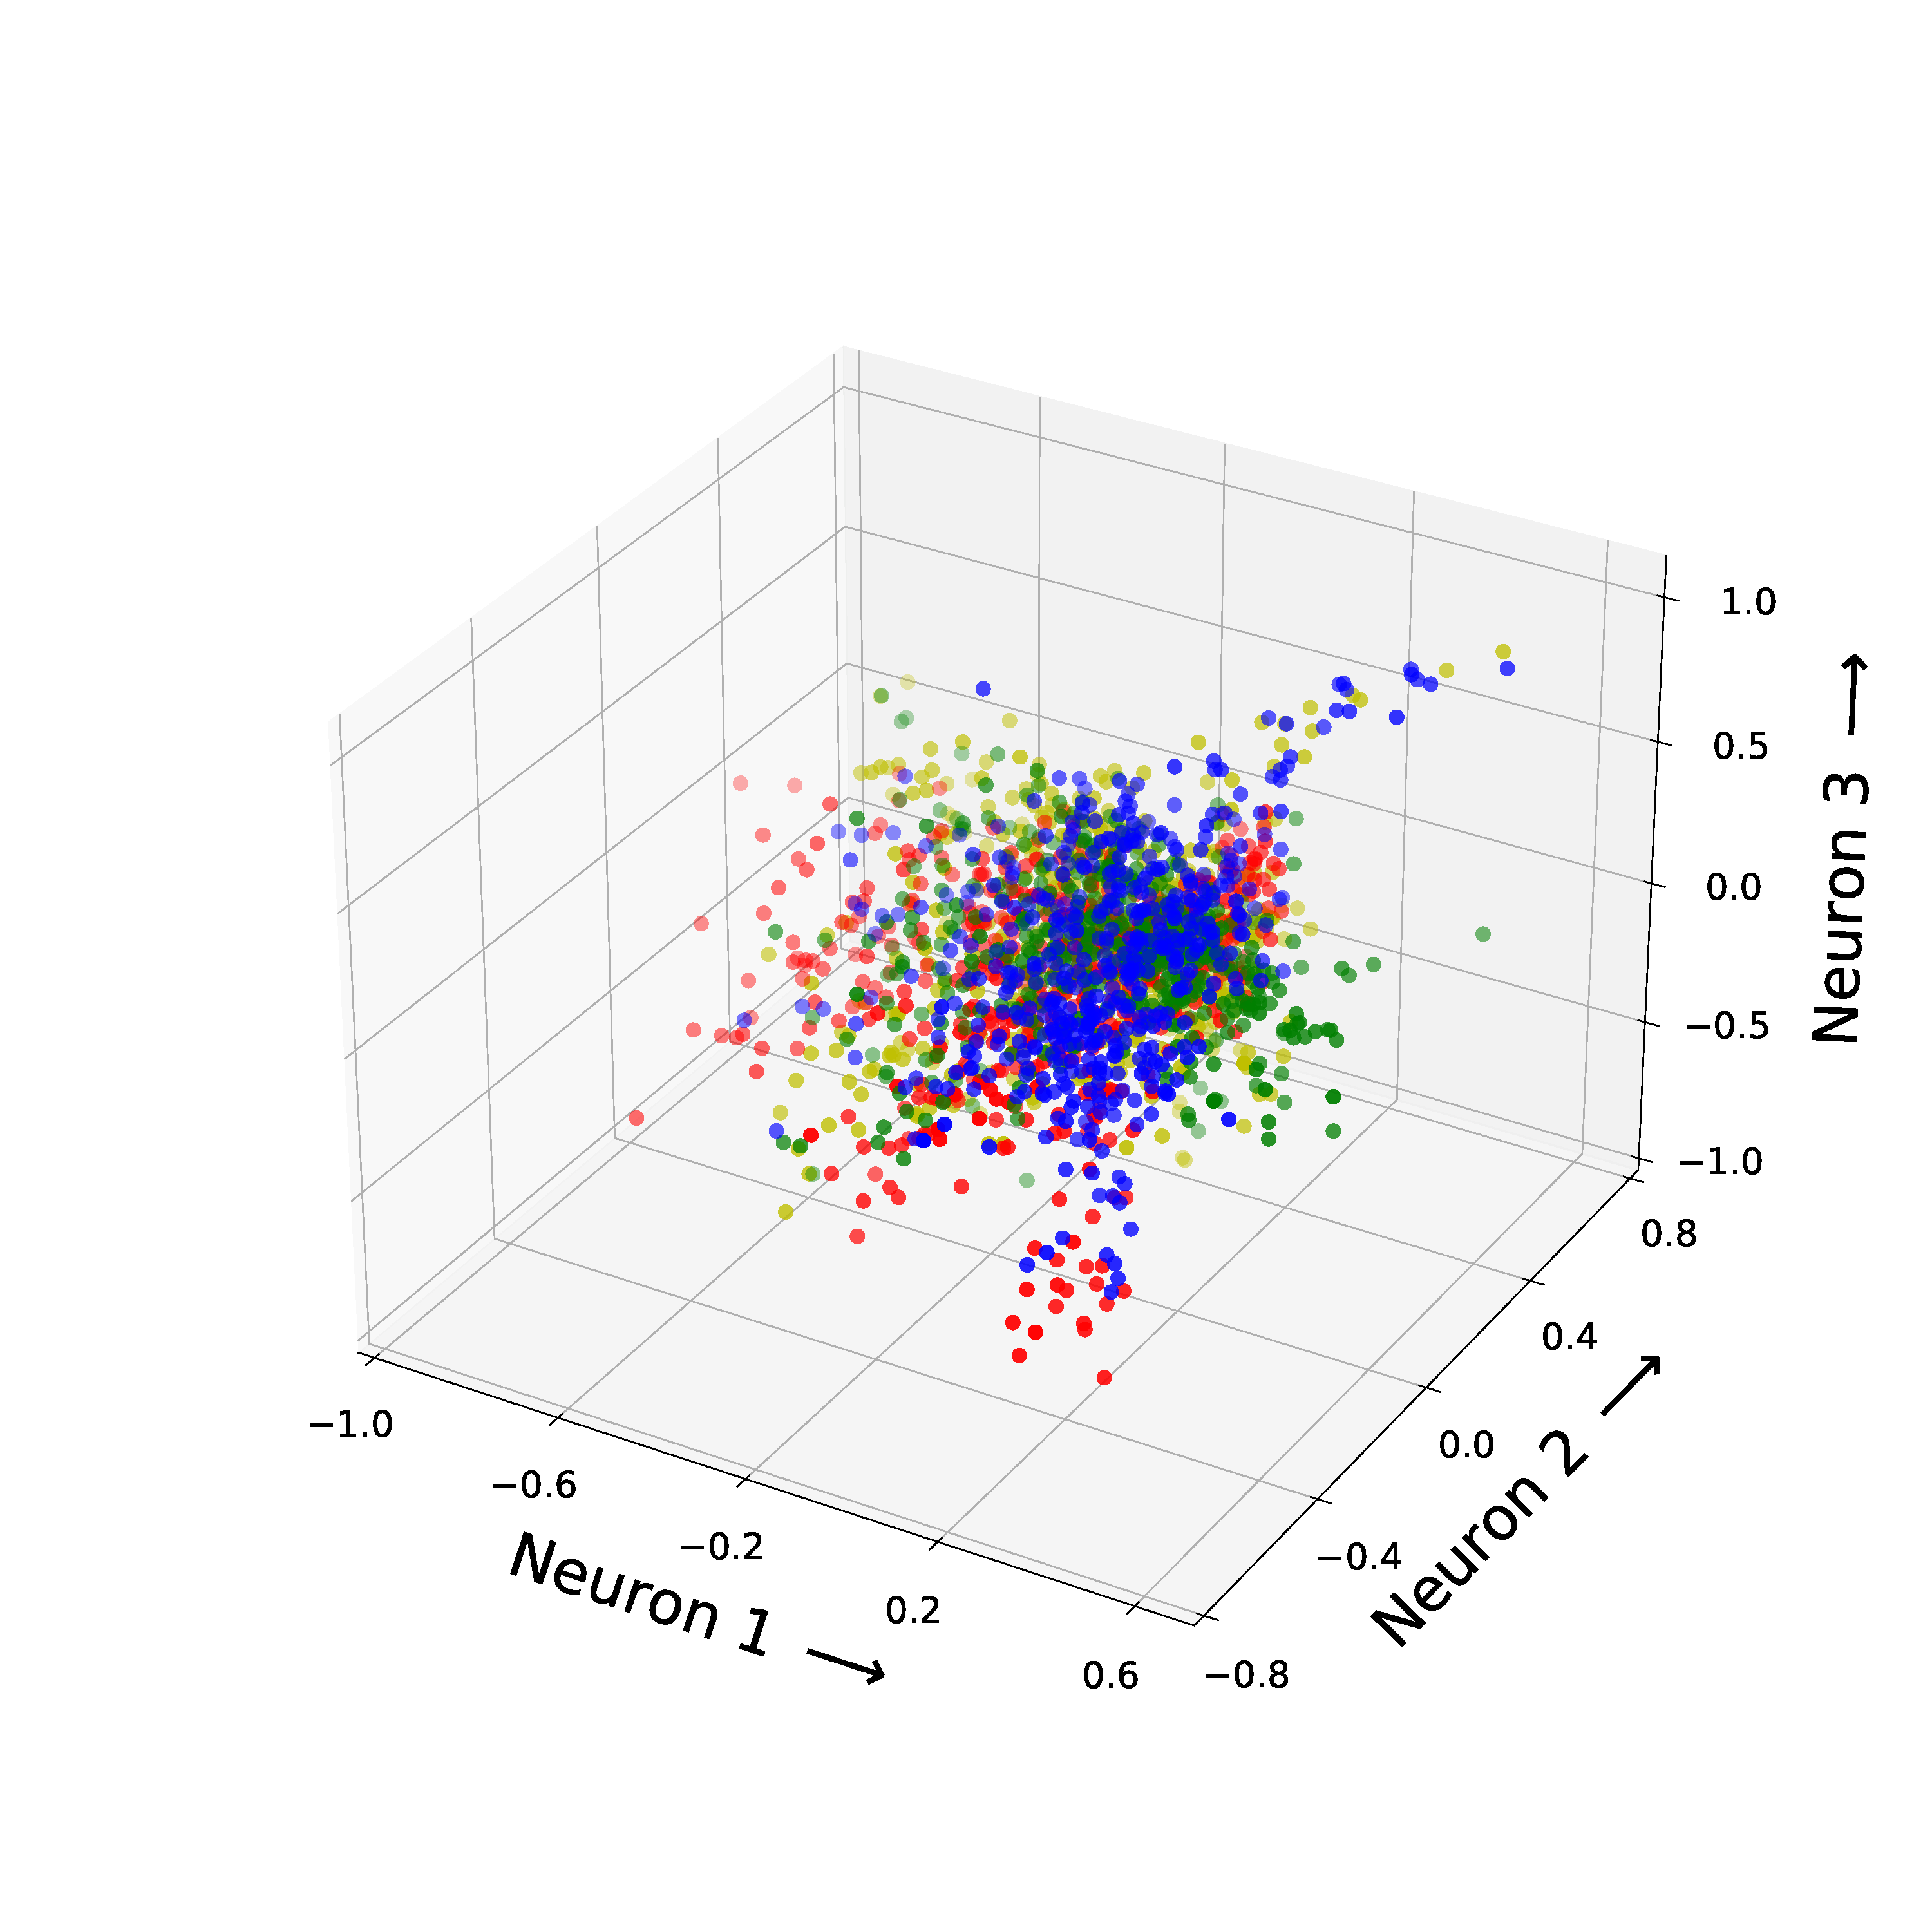
\includegraphics[width=.44\textwidth]{labeled_vs_unlabeled_point_cloud/data_distribution_labeled_mmd_0.pdf}
  \hspace{.4cm}
  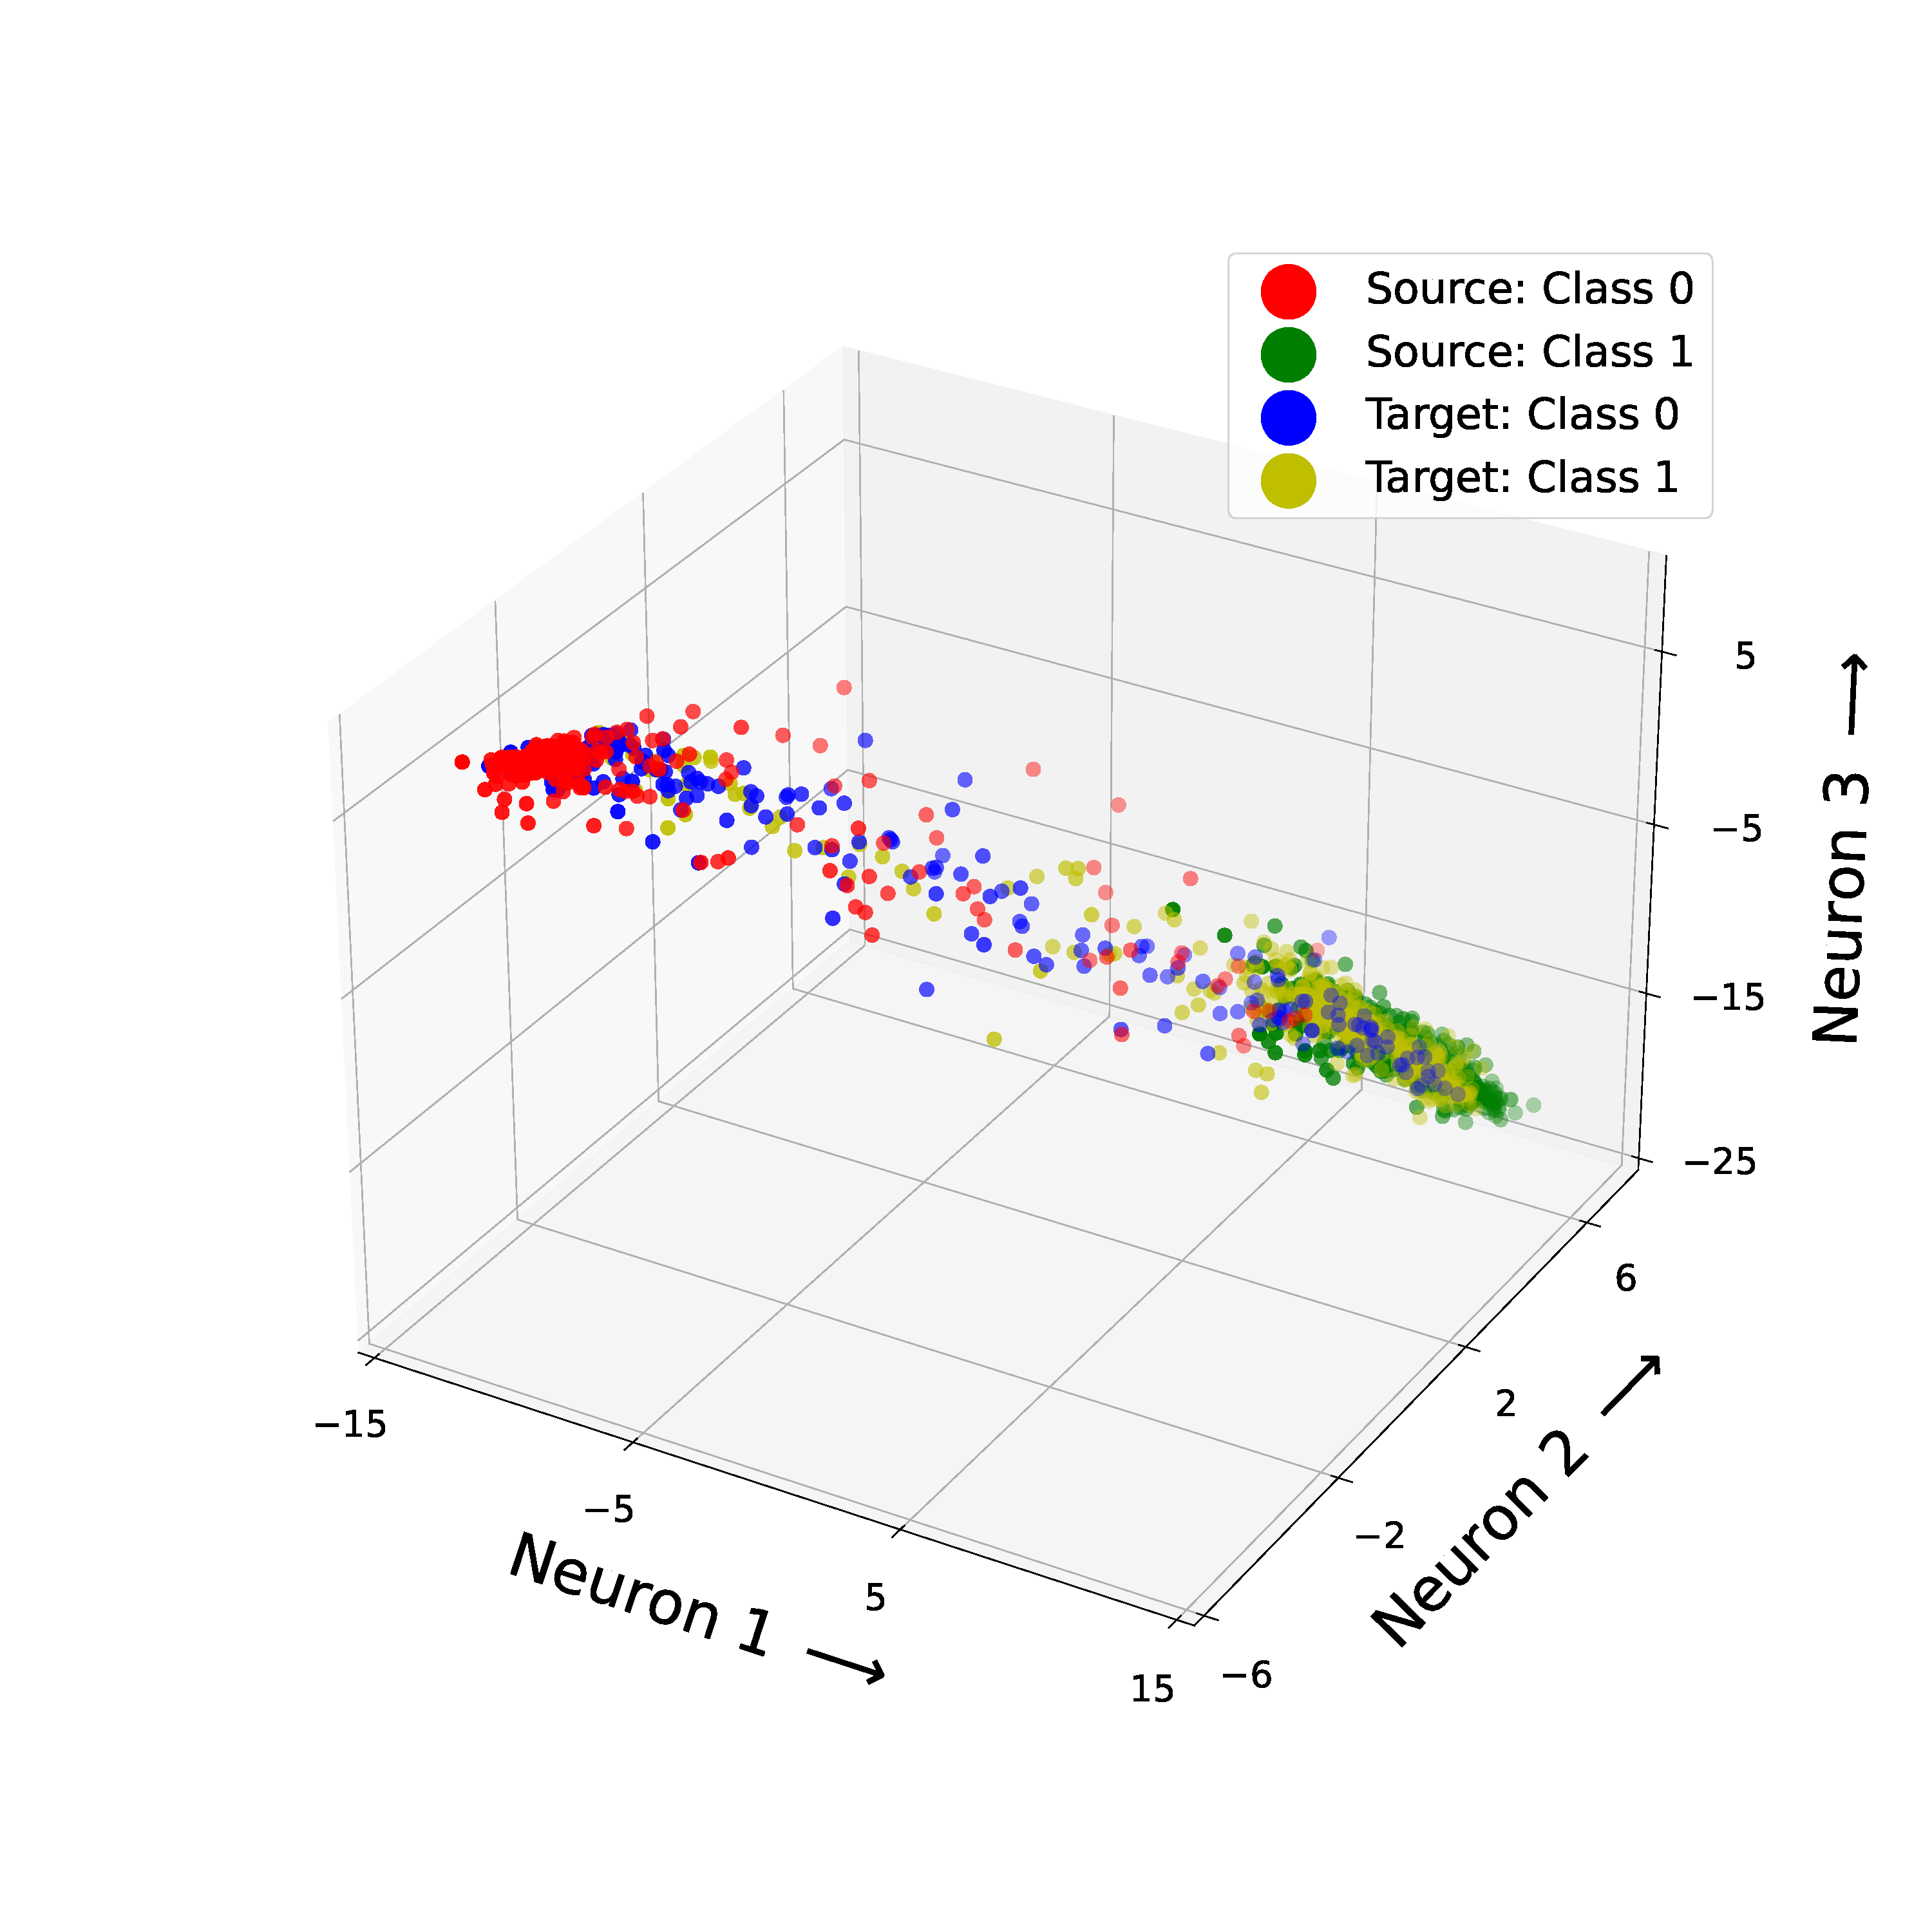
\includegraphics[width=.44\textwidth]{labeled_vs_unlabeled_point_cloud/data_distribution_labeled_mmd_8.pdf}

  \vspace{.1cm}

  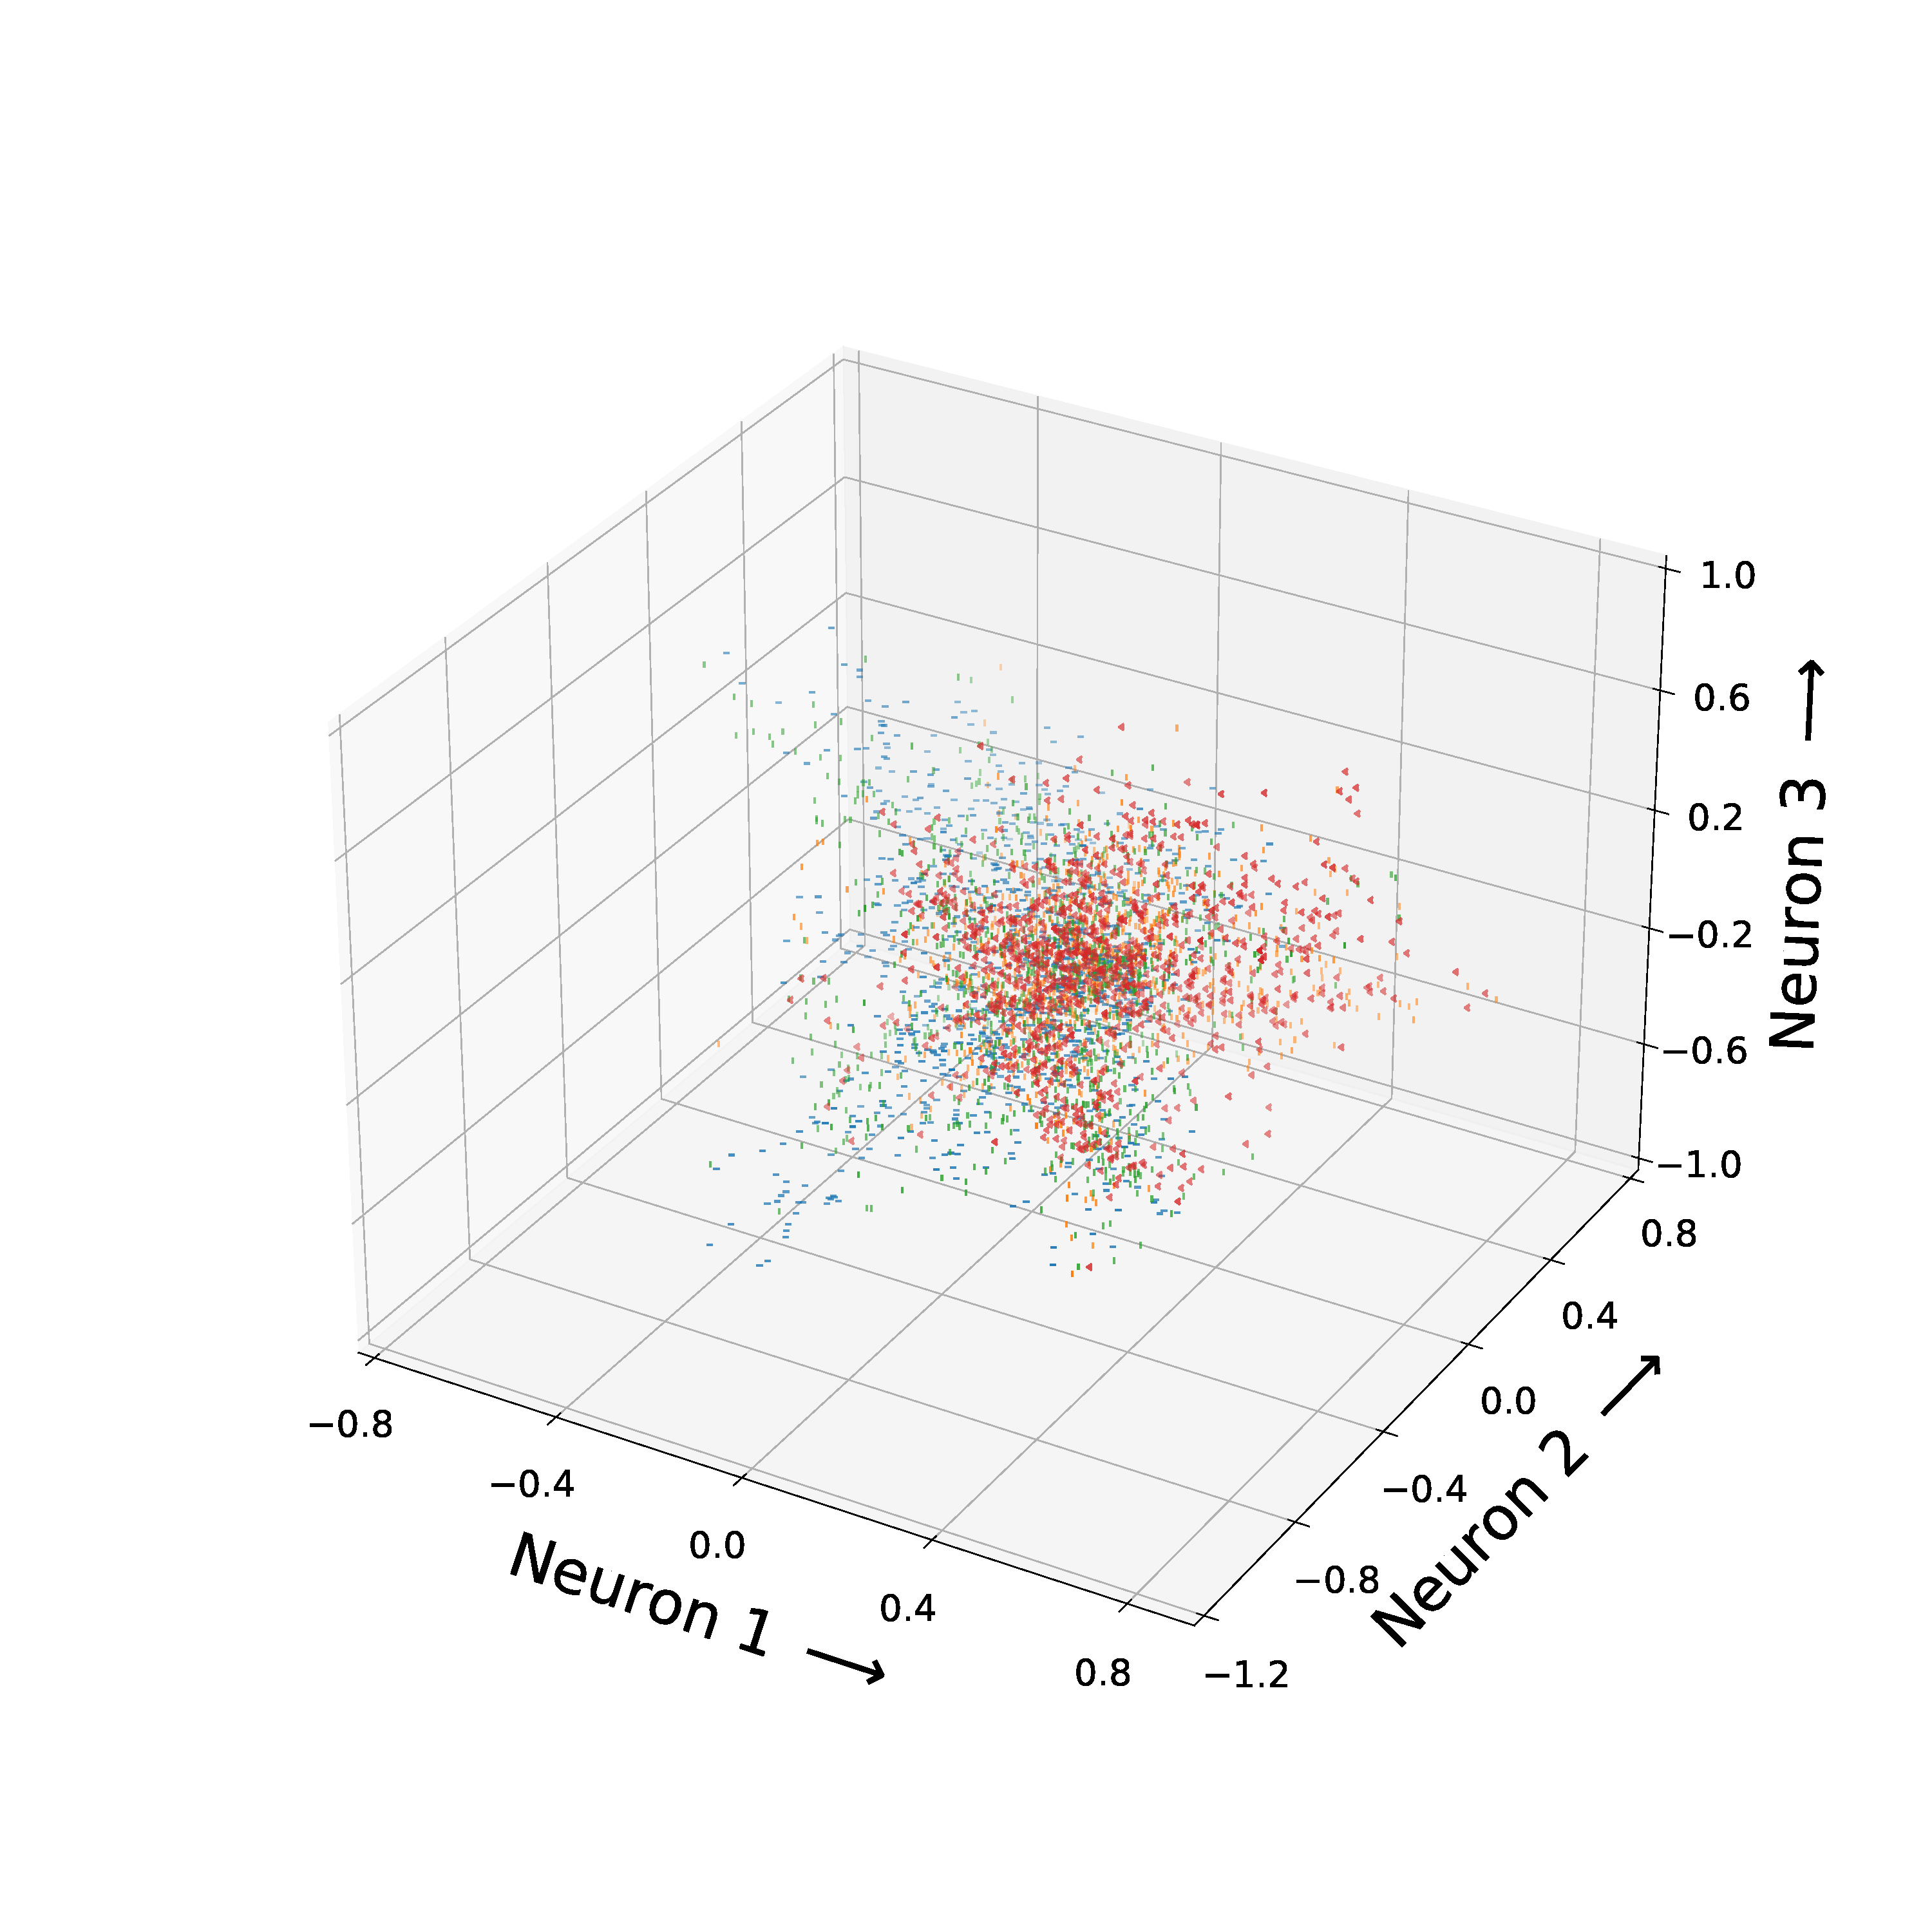
\includegraphics[width=.44\textwidth]{labeled_vs_unlabeled_point_cloud/data_distribution_regular_mmd_0.pdf}
  \hspace{.4cm}
  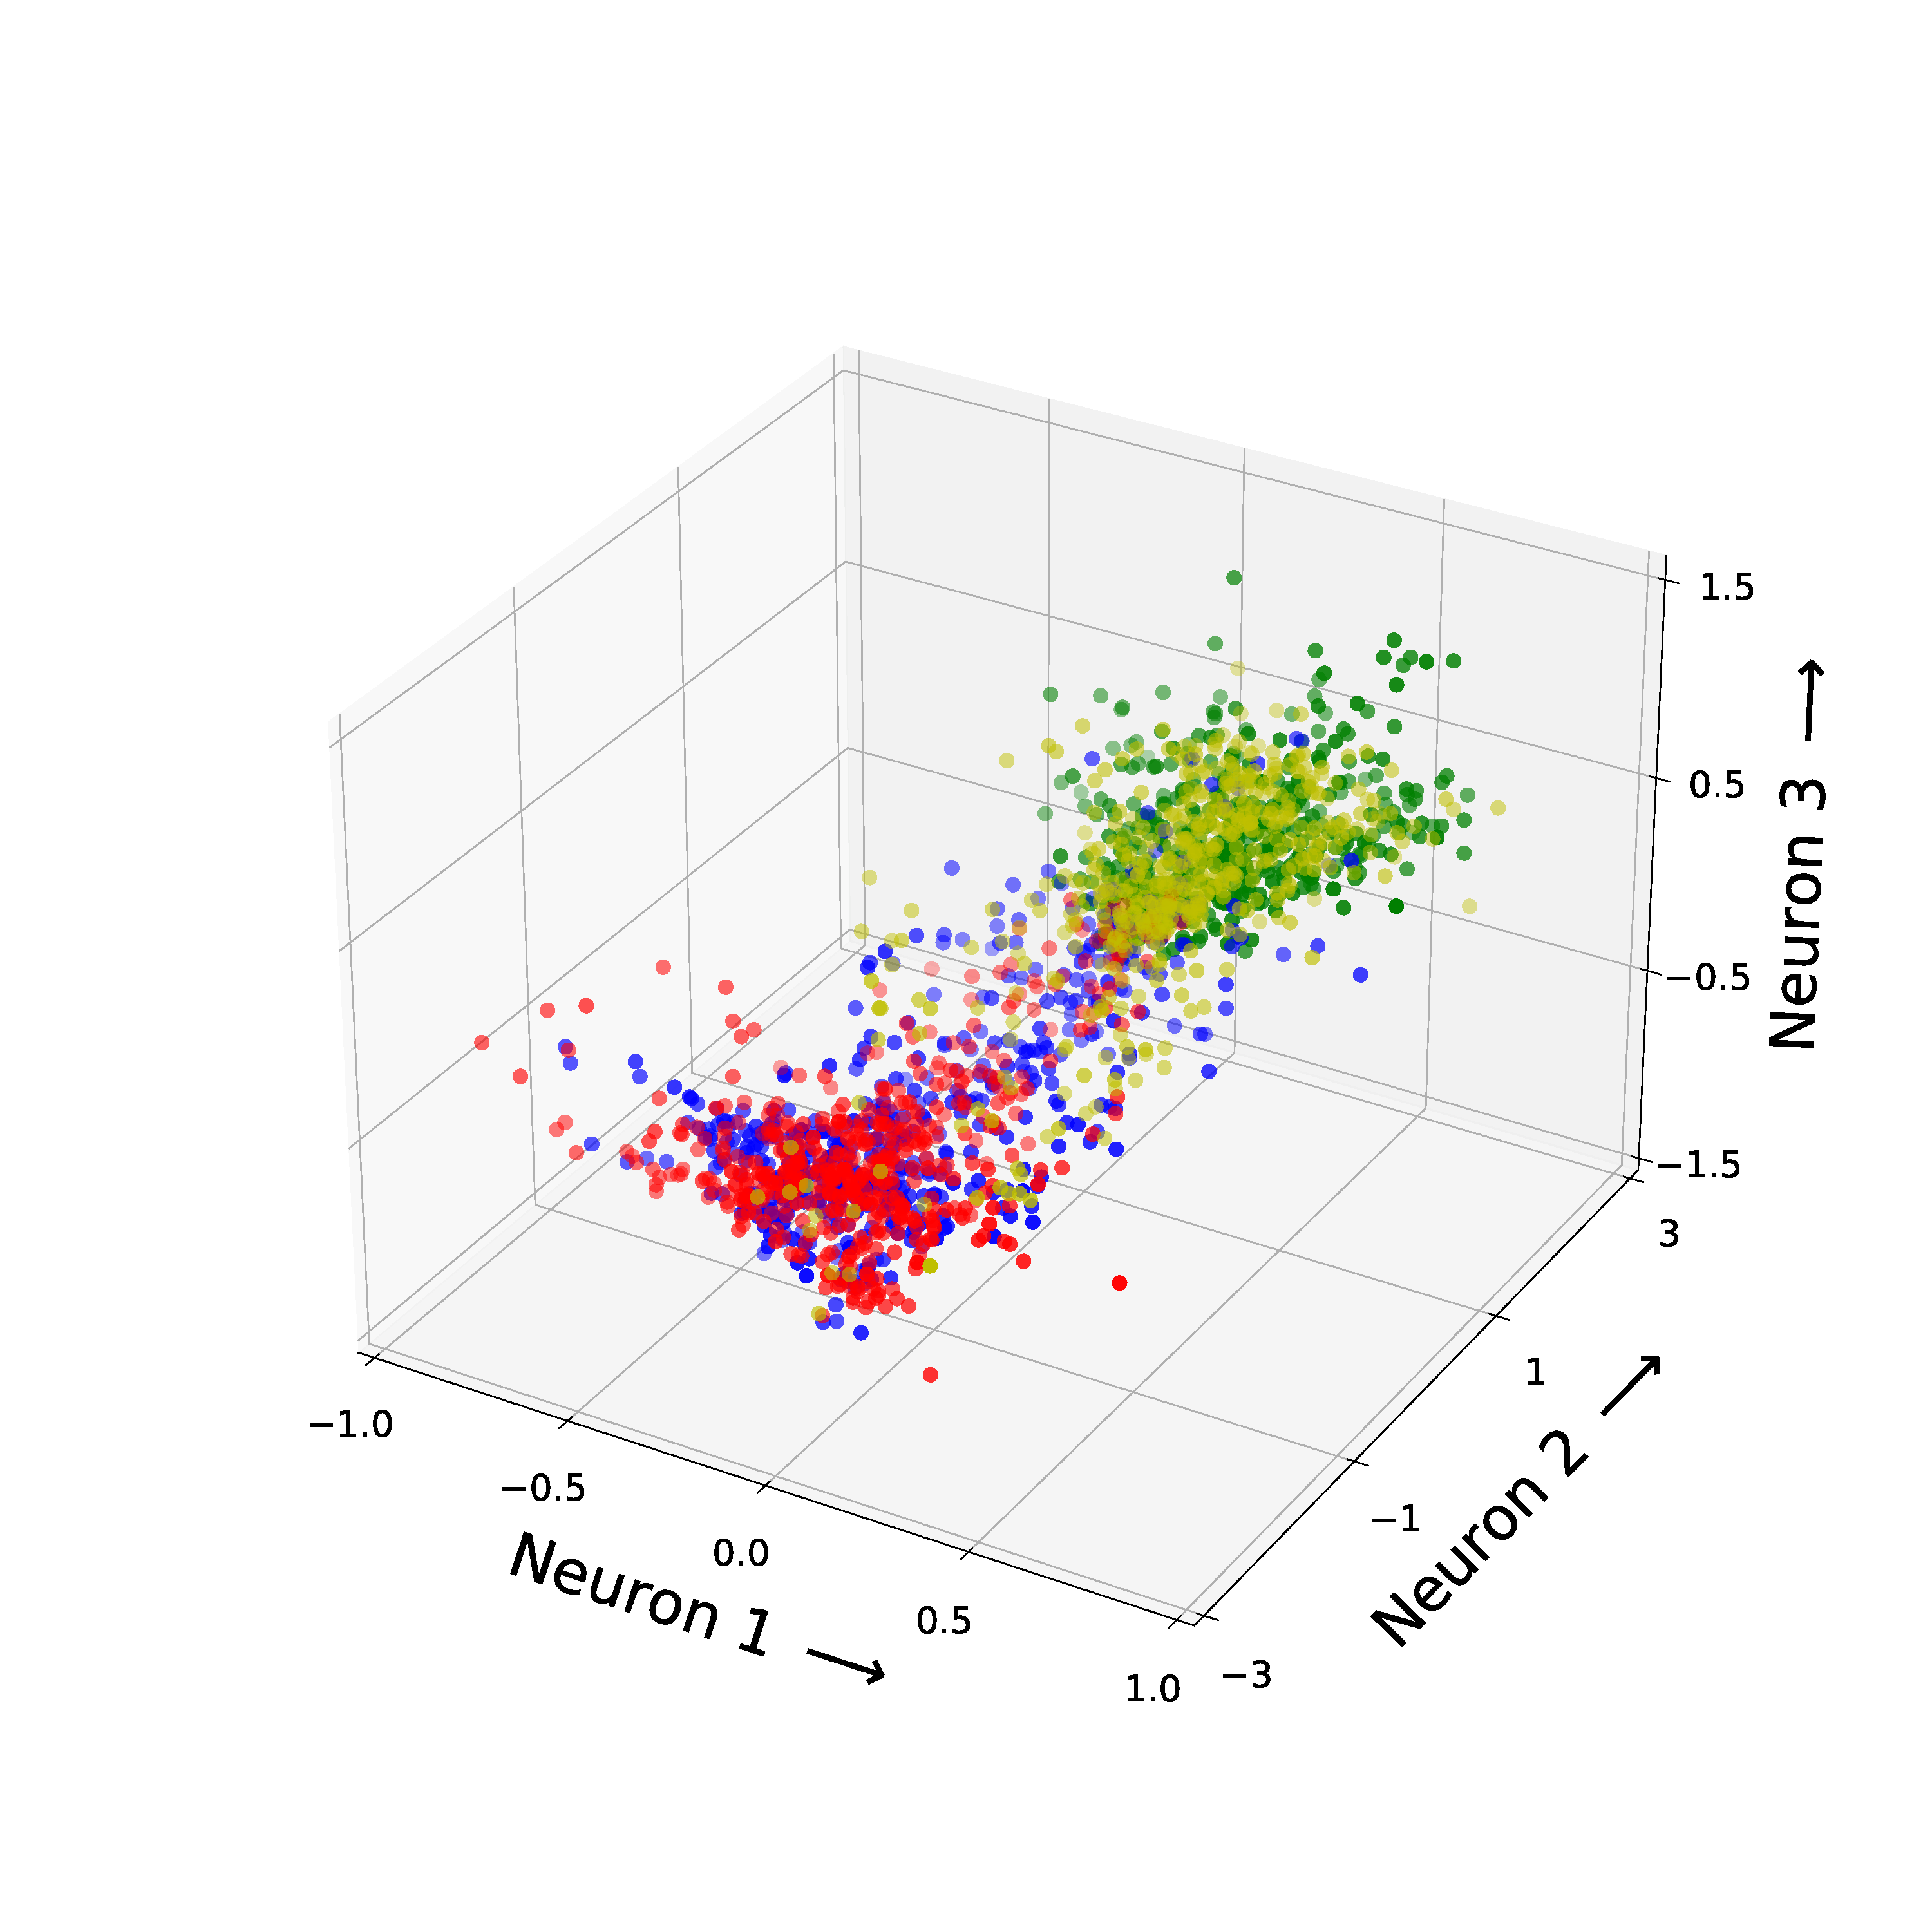
\includegraphics[width=.44\textwidth]{labeled_vs_unlabeled_point_cloud/data_distribution_regular_mmd_8.pdf}
  
  \caption{Data Distribution: Labeled MMD (top) vs. Unlabeled MMD (bottom): Epoch 0 (left) vs. Epoch 8 (right)}
  \label{fig:point_cloud_labeled_unlabeled_mmd}
\end{figure}

\subsection{Influence of Latent Feature Space Choice on the Domain Adaption Performance}
\label{cnn_mmd_dummy}
This section analyzes the influence of applying the MMD-loss in different latent feature maps of the CNN and classifier. The "regular FC MMD" loss calculates the source and target discrepancy from the three latent feature maps in the classifier (flattened output of CNN, FC1, FC2). The "regular FC + CNN MMD" loss additionally considers the feature maps of the three convolutional layers in the CNN (Conv 1, Conv 2 and Conv 3). The accuracy, the source CE and MMD-loss during the training process are shown in fig. \ref{fig:accuracy_cnn_and_no_cnn_mmd} and fig. \ref{fig:loss_cnn_and_no_cnn_mmd}. The accuracies in source and target domain are higher when including the CNN feature maps into the MMD-loss. Besides that, including the CNN feature maps in the MMD-loss increases the stability of the training. The losses, as well as the accuracies, converge faster and smoother.

\begin{figure}[htp]
  \centering
  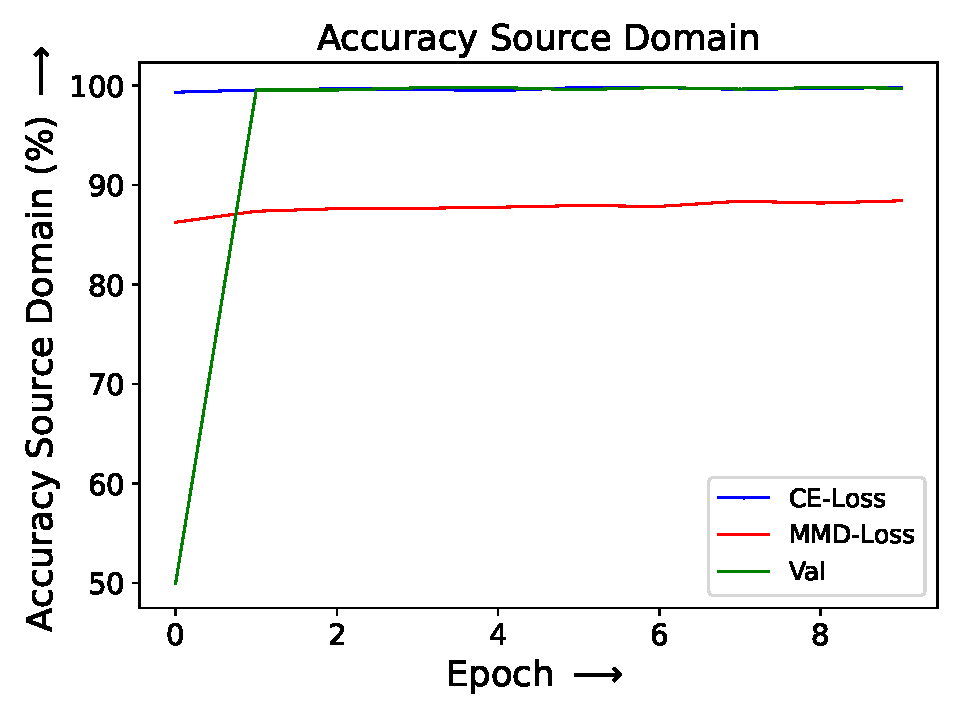
\includegraphics[width=.47\textwidth]{plots_CNN_MMD/Accuracy_Source_Domain_CNN_MMD.pdf}
  \hspace{.3cm}
  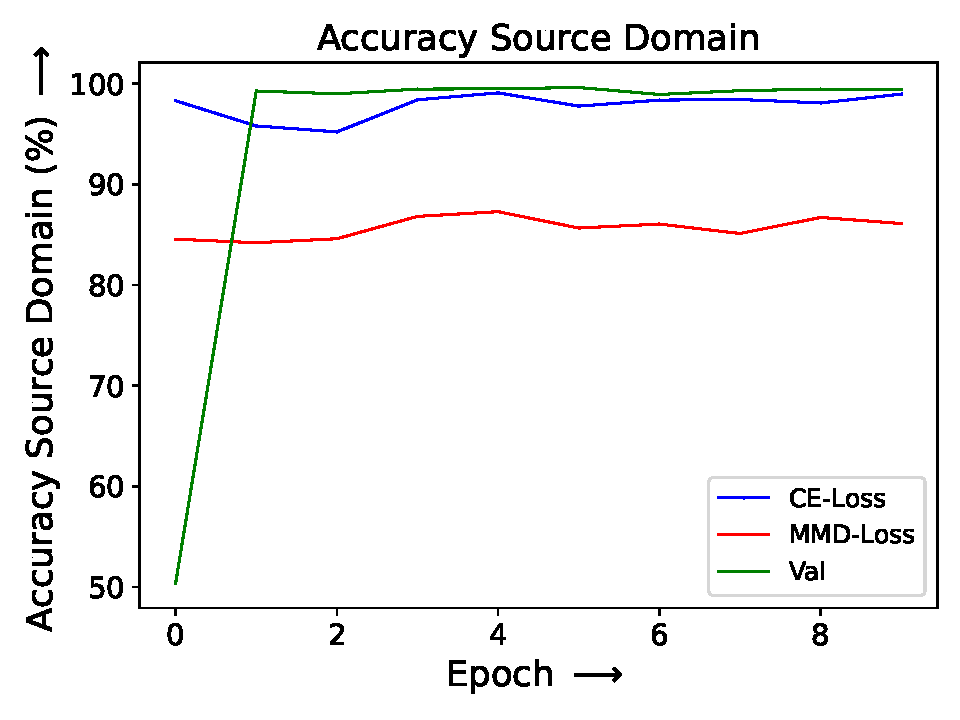
\includegraphics[width=.47\textwidth]{plots_CNN_MMD/Accuracy_Source_Domain_FC_MMD.pdf}

  \vspace{.1cm}

  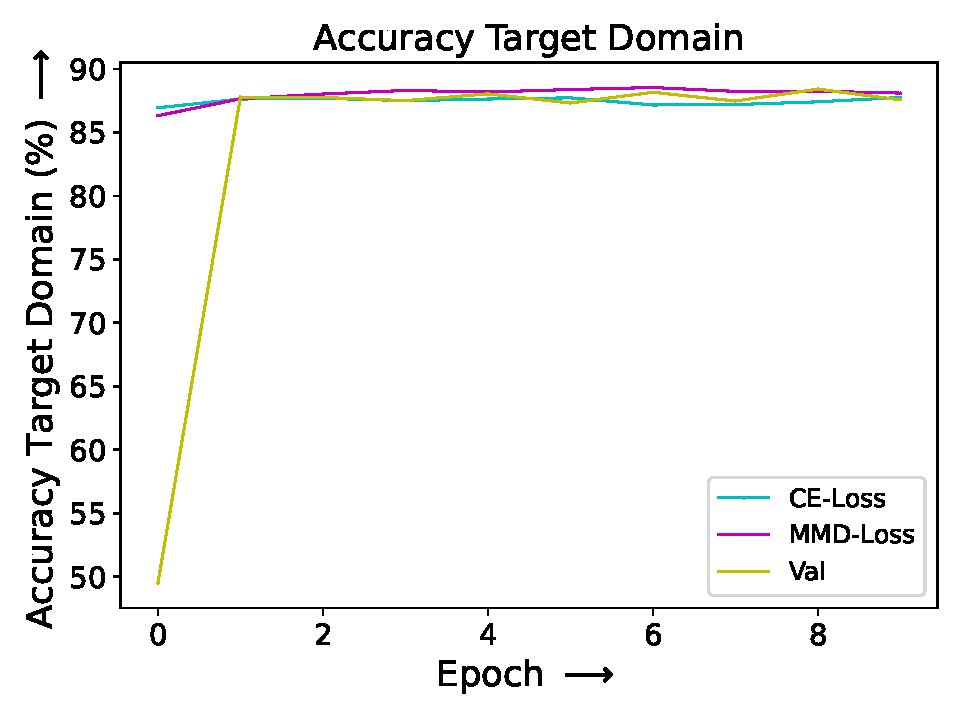
\includegraphics[width=.47\textwidth]{plots_CNN_MMD/Accuracy_Target_Domain_CNN_MMD.pdf}
  \hspace{.3cm}
  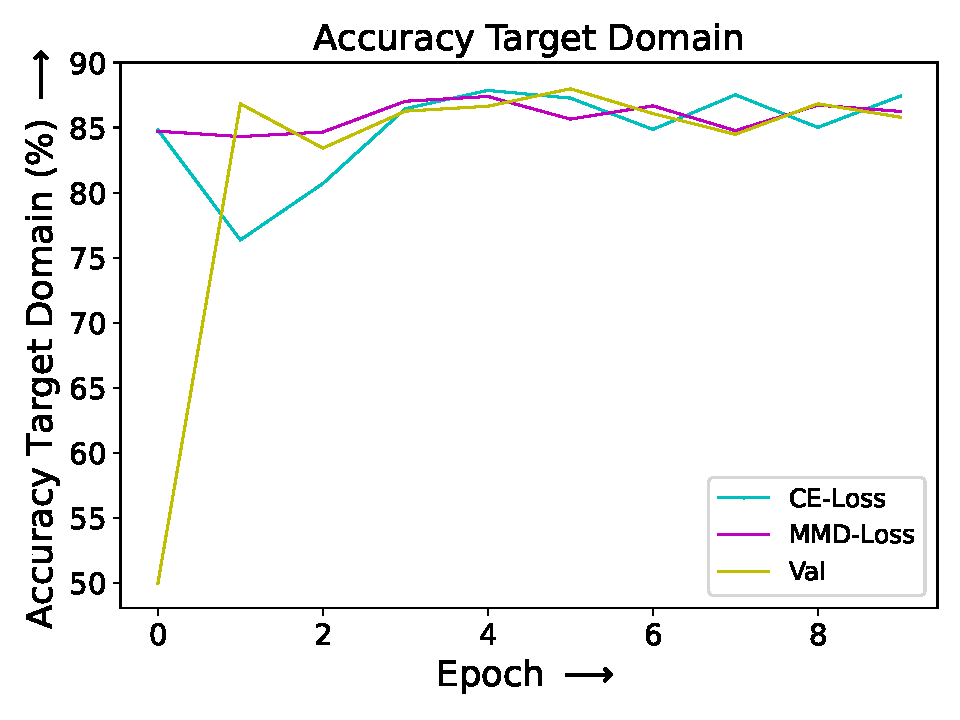
\includegraphics[width=.47\textwidth]{plots_CNN_MMD/Accuracy_Target_Domain_FC_MMD.pdf}

  \caption{Source and Target Accuracy: MMD in CNN (left), MMD in FC (right)}
  \label{fig:accuracy_cnn_and_no_cnn_mmd}
\end{figure}

\begin{figure}[H]
  \centering
  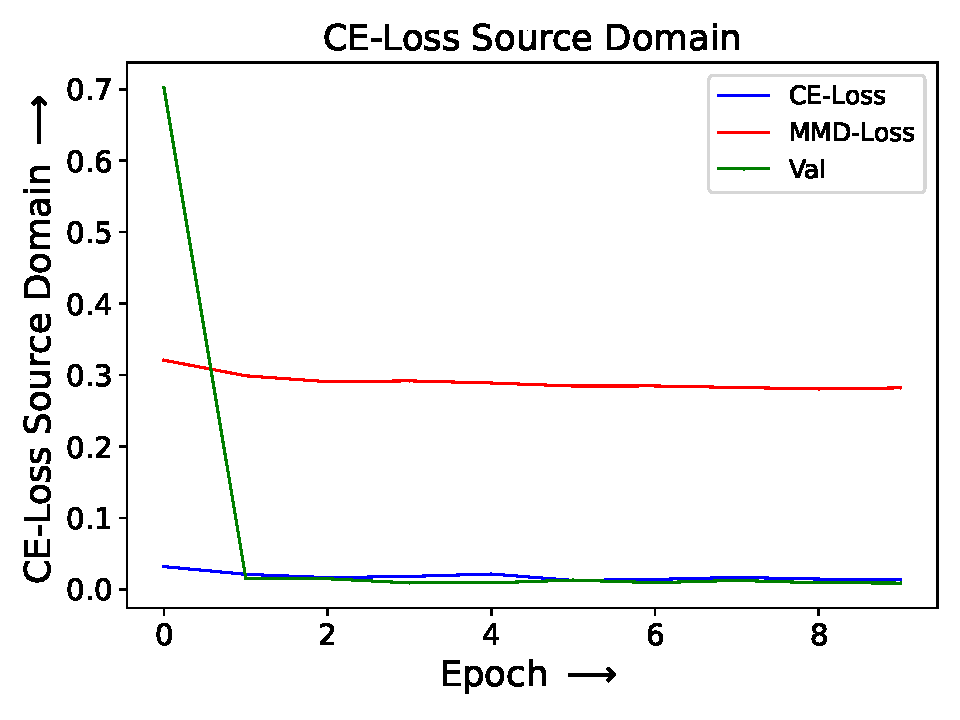
\includegraphics[width=.47\textwidth]{plots_CNN_MMD/CE_Loss_Source_Domain_CNN_MMD.pdf}
  \hspace{.3cm}
  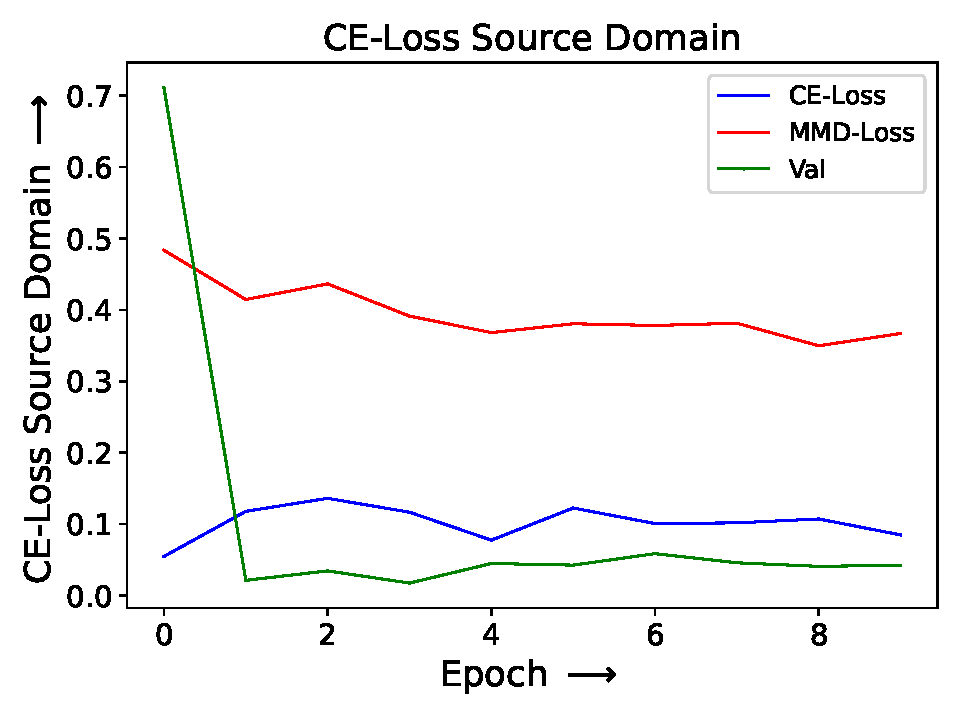
\includegraphics[width=.47\textwidth]{plots_CNN_MMD/CE_Loss_Source_Domain_FC_MMD.pdf}

  \vspace{.1cm}

  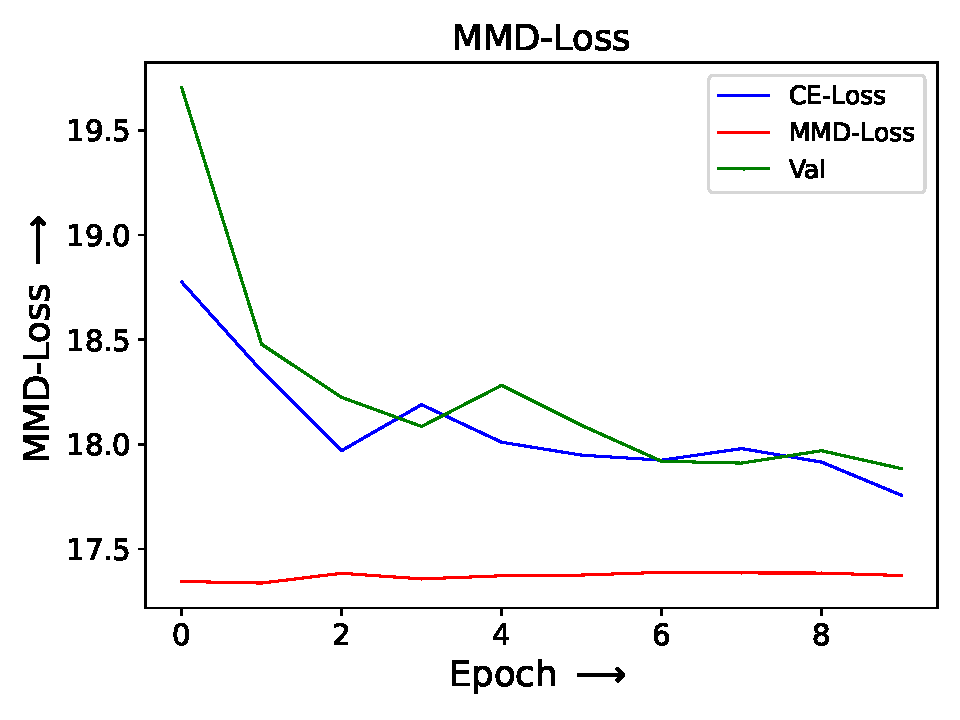
\includegraphics[width=.47\textwidth]{plots_CNN_MMD/MMD_Loss_CNN_MMD.pdf}
  \hspace{.1cm}
  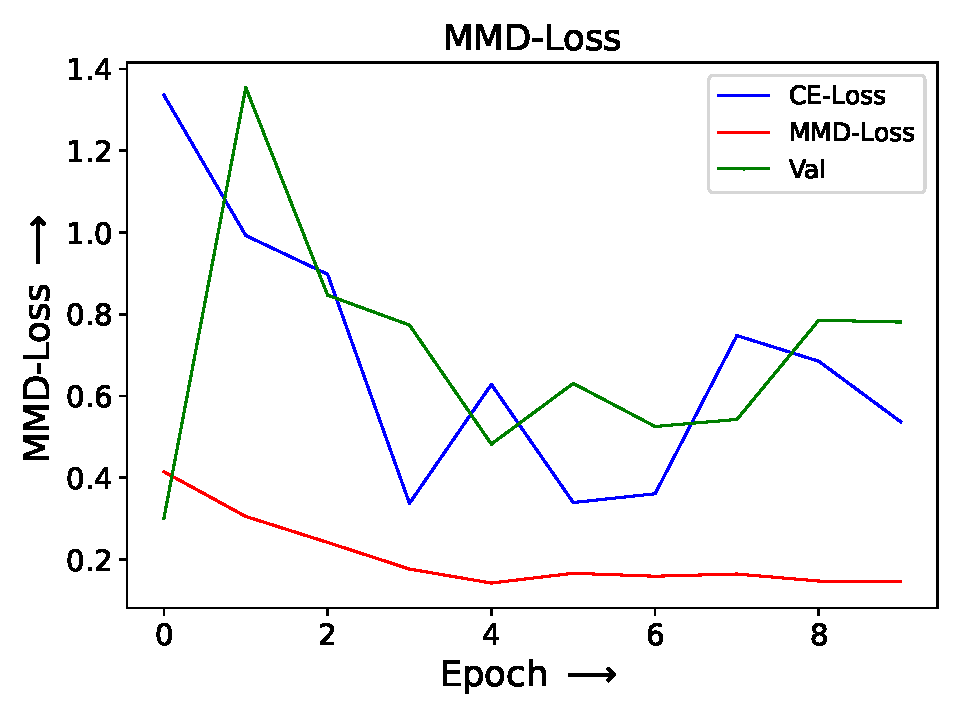
\includegraphics[width=.48\textwidth]{plots_CNN_MMD/MMD_Loss_FC_MMD.pdf}

  \caption{MMD- and CE-Loss: MMD in CNN (left), MMD in FC (right)}
  \label{fig:loss_cnn_and_no_cnn_mmd}
\end{figure}

By passing data through the model, features with varying levels of abstraction are extracted. Supervising the domain discrepancy in feature maps of different abstraction levels seems reasonable. Generally, shallow layers in neural network extract more global and deeper more task-specific features. Deeper layers often suffer from stronger domain-dependencies. Since each layer in a neural network influences subsequent layers, it makes sense to apply the MMD-loss early in the network. Reducing the domain discrepancy in shallow layers makes the network extract more domain-invariant features in all following layers as well. Especially in challenging tasks with strong domain discrepancies, it is reasonable to intervene early. Reducing the domain discrepancy just in the final layers of the model leads to a less stable and smooth optimizations. Potentially, the MMD and source CE-loss tend to be more contradicting when applied in these layers. The two training goals, which seem to work against each other, make the optimization more fluctuating. During the optimization, different strong local minima coming from one of the two losses might be found. The model performance sometimes breaks down after some stable epochs of constant training. One has to remember calculating the regular FC + CNN MMD-loss is quite expansive since the feature maps extracted from the convolutional layers are complex and high-dimensional.



\section{Real-World Dataset}
In the following section the performance of different MMD-based domain adaption models are evaluated on the real-world BSD dataset. The goal of this chapter is to evaluate the benefits and problems of the presented approach for PHM on industrial machines. All presented models have the same architecture but differ in their optimization processes. Different GAMMA and MMD layer choices were evaluated. The performance of each model is compared with the baseline model, which does not use any MMD-loss during training. For each model, the following table shows, in which latent feature spaces a MMD-loss was applied:

\begin {table}[H]
\centering

\begin{tabular}{llllllll}
  \toprule
  Model          & Conv1 & Conv2 & Conv3 & FC1 & FC2 & FC3 \\
  \midrule
  
\vspace{.5cm}

 \parbox[t]{0mm}{\multirow{1}{*}{\rotatebox[origin=c]{90}{\thead{BASE- \\ LINE}}}} & - & - & - & - & - & -\\
 
\vspace{.5cm}

 \parbox[t]{0mm}{\multirow{1}{*}{\rotatebox[origin=c]{90}{\thead{FULL \\ MMD}}}} & \checkmark & \checkmark & - & \checkmark & \checkmark & \checkmark\\
 
\vspace{.5cm}

 \parbox[t]{0mm}{\multirow{1}{*}{\rotatebox[origin=c]{90}{\thead{FC \\ MMD}}}} & - & - & - & \checkmark & \checkmark & \checkmark\\
 
\vspace{.5cm}

 \parbox[t]{0mm}{\multirow{1}{*}{\rotatebox[origin=c]{90}{\thead{CNN \\ MMD}}}} & \checkmark & \checkmark & \checkmark & - & - & -\\

 
  \bottomrule
\end{tabular}

\caption {MMD layer choice of presented models} \label{tab:MMD_layer_choice} 
\end {table}

Similarly to the dummy dataset, the influence of GAMMA and the MMD layer choice on the PHM performance are examined in the chapter \ref{ch:Influence_GAMMA_real_dataset} and \ref{ch:Influence_Layer_real_dataset}. Since the previously presented labeled MMD-loss uses target labels, which all other models do not, the labeled MMD-loss model was not included in the evaluation on the real data. To achieve good comparability just models with equal training conditions and access to data are considered. Besides that, the labeled MMD loss has additional hyperparameters which balance the optimization of the domain discrepancy between source and target samples of the same and different classes. Tuning the labeled MMD-loss for a new task is therefore more complicated and expects further experiments to find appropriate hyperparameters. Due to the limited time in the thesis the focus of the investigations on the real-world dataset lies in the regular MMD-loss. In the chapter \ref{ch:PHM_performance} the actual performance of different models for the PHM task on BSDs is evaluated by the target accuracy on the test data. For the implementation of the presented models, PyTorch was used.  All computations were performed on a Leibniz Supercomputing Centre7 compute node virtual machine with 20
Intel® Xeon® Gold 6148 vCPUs, one Nvidia® Tesla V100, 368 GB RAM, PyTorch v.1.4.0 and CUDA 10.1


\begin{comment}
In the following section the performance of different MMD-based domain adaption approaches are evaluated on the real-world ball screw drive dataset. The model used for this evaluation is presented in fig. \ref{fig:model_real_data}. From the 49 features in the dataset just three (\verb|'C:x_bottom'|, \verb|'C:y_bottom'|, \verb|'C:z_bottom'|) are used. For this reasons three sequences of length 1024 are fed into the CNN.

\begin{figure}[H]
  \centering
  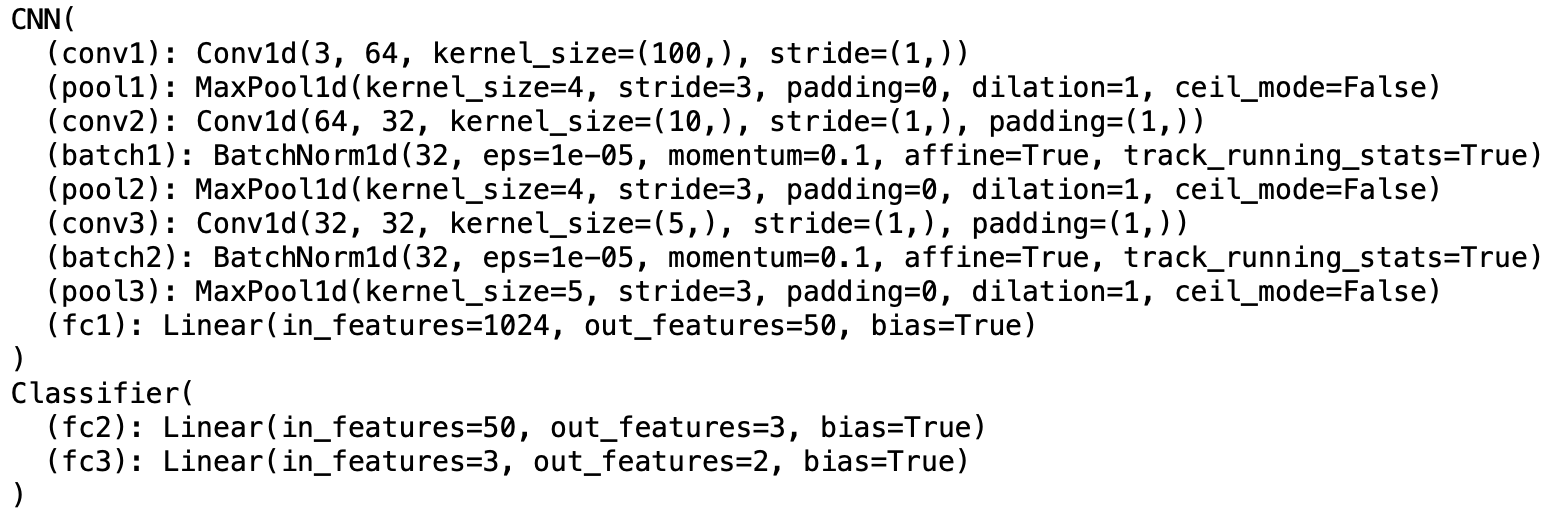
\includegraphics[width=1.1\textwidth]{model_real_data}
  \caption {MMD Model for Real Dataset} \label{fig:model_real_data}
\end{figure}


On the real machine dataset the three approaches regular FC + CNN MMD-loss,  regular FC MMD and no MMD-loss are evaluated. The accuracies on the source and target domain are visualized in fig. \ref{fig:accuracy_real_world}. In each figure three curves are presented representing different phases of the training. During the MMD-loss phase the whole model consisting of CNN and classifier are optimized with a weighted average of MMD and CE loss. In the CE-loss phase just the classifier is optimized according to a CE-loss. During both phases an ADAM optimizer with a learning rate of 1e-2, beta1 of 0.9 and beta2 of 0.99 is used . In the val phase the model is evaluated. Before the training the data is split for these three phases accordingly (MMD-loss: 60\%, CE-loss: 20\%, Val: 20\%). Therefore all experiments follow a proper train validation split. It becomes obvious that the accuracies achieved on the validation set of the target domain were able to be increased with about 10\% by using the two MMD variations. The MMD and CE-loss seems to be decreased more smoothly when including CNN features into the MMD-loss for the optimization of the model. Also the accuracy achieved on the target validation set achieved the regular FC + CNN MMD-loss beat the one achieved with the regular FC MMD-loss. Without using any MMD-loss the model performance on the target domain could be increased by just around 2\%. When using the regular FC MMD-loss sometimes the performance of the model breaks down  little bit. Often times this can be seen in the accuracy of the target and source domain. An example for this phenomena can be seen in fig. \ref{fig:accuracy_real_world} when looking at the accuracies of regular FC MMD (middle). In epoch ~27 the accuracy breaks down on the target and source domain. Especially during the combined training with the MMD and CE loss this effect becomes especially obvious. Like mentioned in previous chapters this shows that when not including the latent features of the CNN in the MMD-loss the CE and MMD-loss seem to work against each other, which makes the optimization less stable.

\begin{figure}[H]
  \centering
  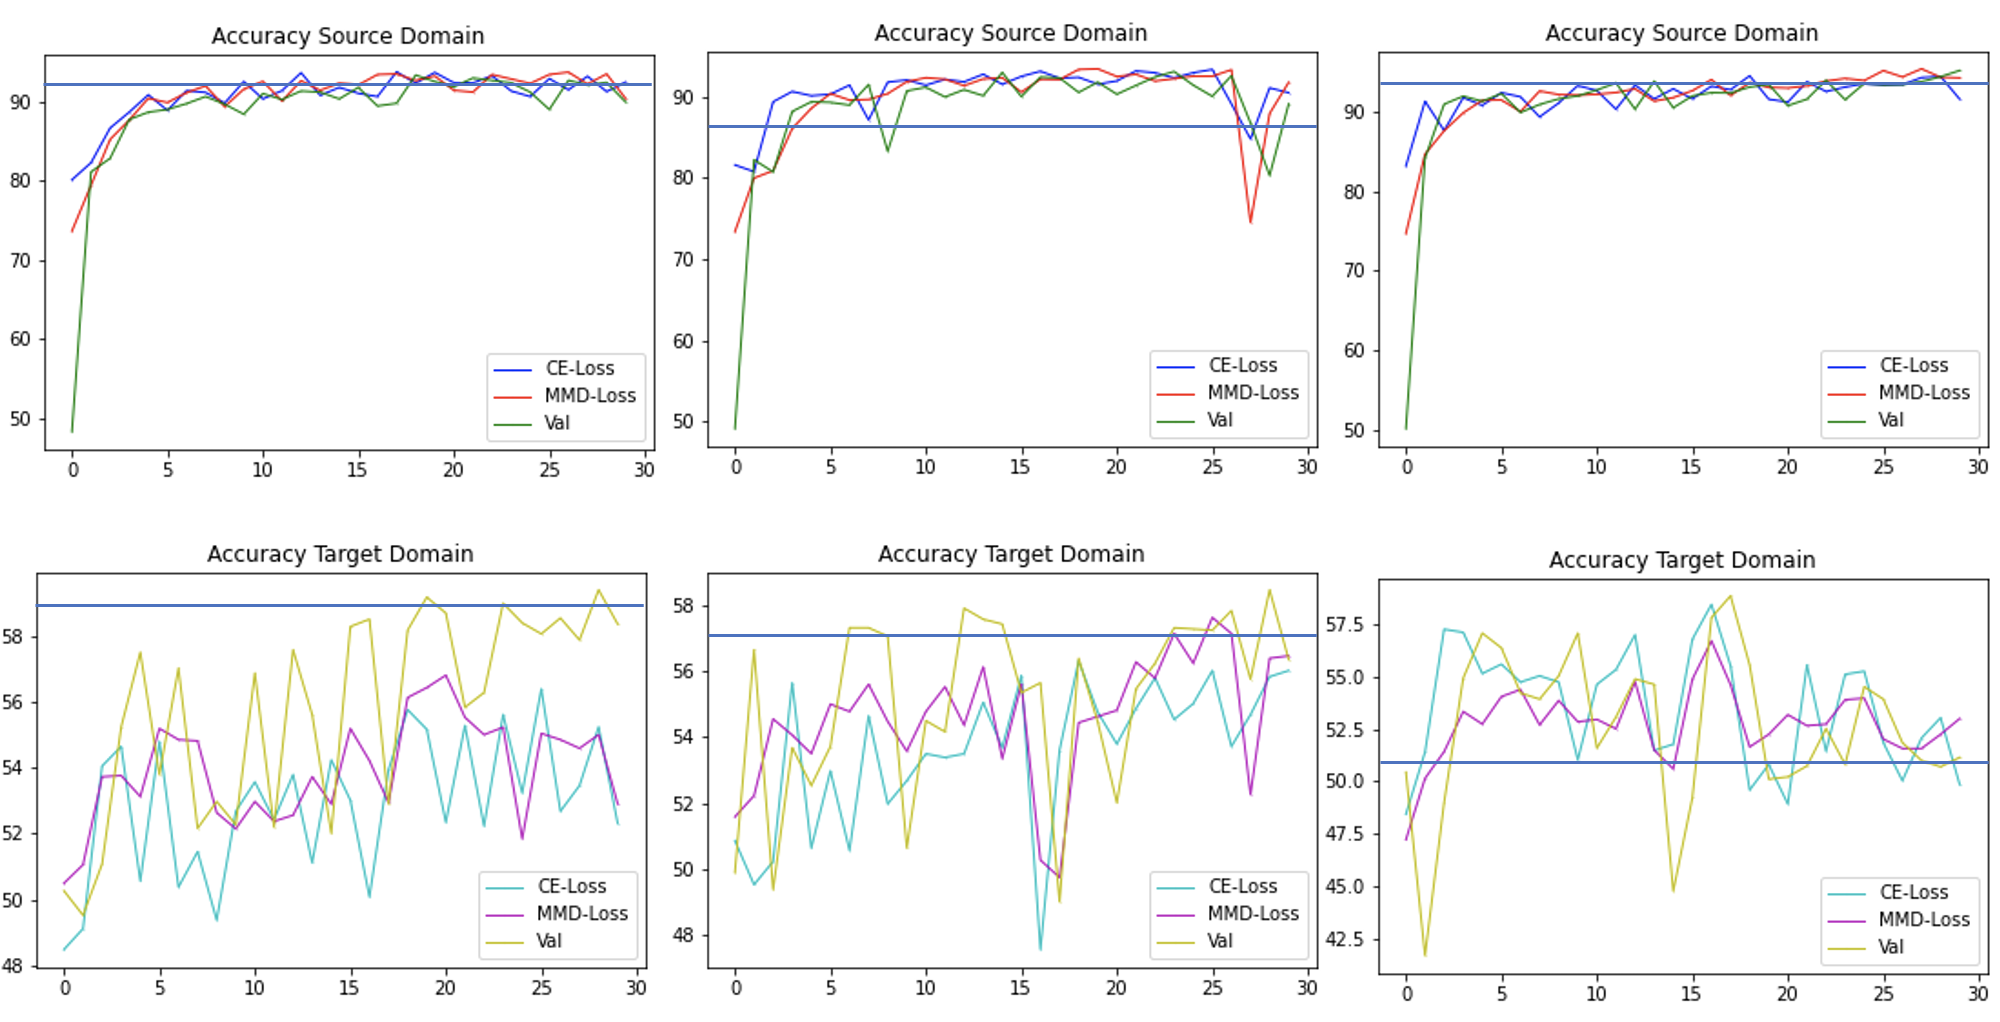
\includegraphics[width=1.1\textwidth]{accuracy_real_world}
  \caption {Source and Target Accuracies for model training with Regular FC + CNN MMD-loss (left), Regular FC MMD (middle) and No MMD-loss (right)} \label{fig:accuracy_real_world}
\end{figure}


\begin{figure}[H]
  \centering
  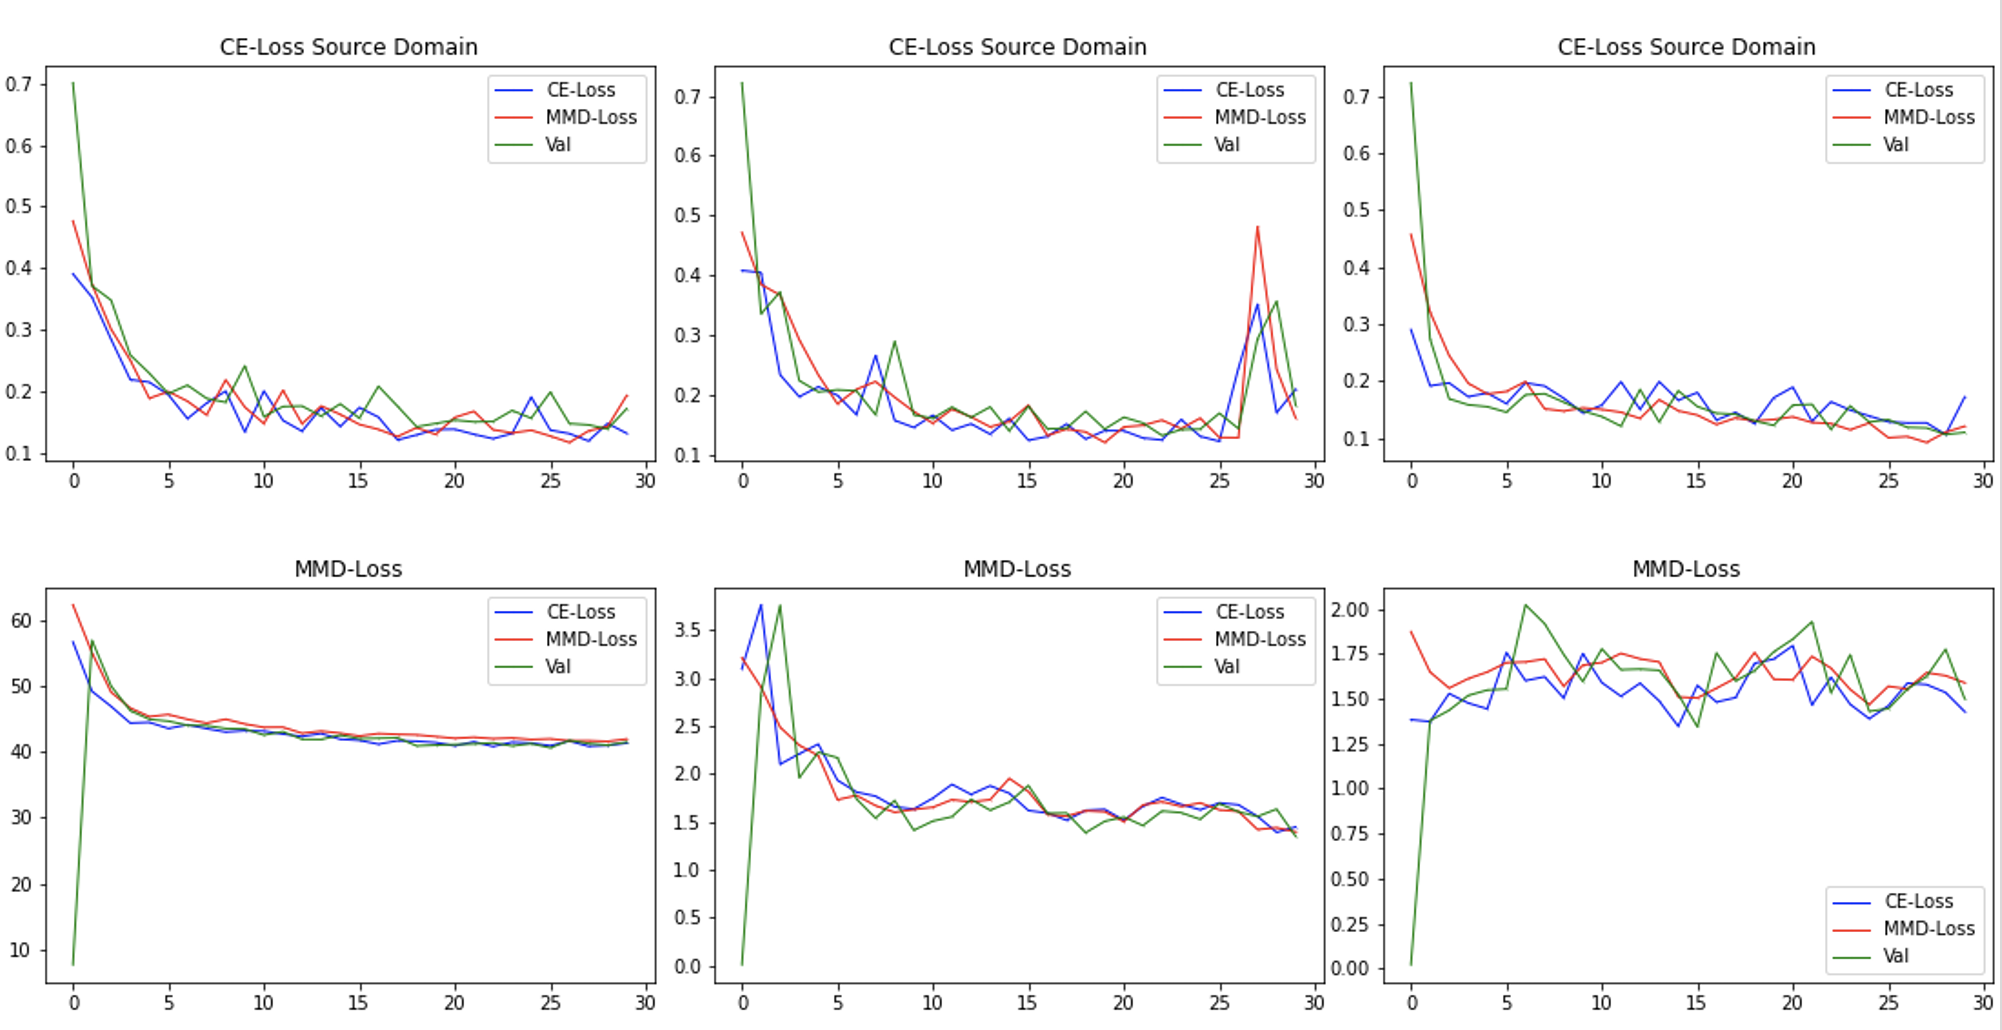
\includegraphics[width=1.1\textwidth]{loss_real_world}
  \caption {Loss for model training with Regular FC + CNN MMD-loss (left), Regular FC MMD (middle) and No MMD loss} \label{fig:loss_real_world}
\end{figure}


In fig. the development of the source CE and MMD-loss is shown. It can be seen, that the hyperparameter GAMMA was picked well, such that the MMD as well as the source CE-loss were able to be reduced smoothly throughout the trainings process. 


Unfortunately the MMD-loss could just minimize the domain discrepancy by a little. The domain discrepancy problem couldn't be solved completely. Still the idea of the MMD-loss becomes more clear in the experiments. Also the positive effect of the MMD-loss for the training is obvious. For the complex multi-dimensional dataset the MMD-loss is probably not sophisticated enough to detect and effectively fight the domain discrepancy.
\end{comment}






\subsection{Influence of GAMMA Choice on the PHM Performance}\label{ch:Influence_GAMMA_real_dataset}

In the following three models are trained with a full MMD-loss and different GAMMAs (0.05, 0.4, 20). The models were trained on the  D:P mech./X signal for 100 epochs. Similarly to the dummy dataset, the model training is very sensitive to the GAMMA choice. Just when GAMMA is chosen correctly, the source CE and MMD-loss can be reduced simultaneously. Both training goals, reducing the domain discrepancy in the models hidden layer and classifying the source domain samples correctly, can be pursued in parallel. Fig. \ref{fig:distribution_GAMMA_influence_real_data} shows the latent feature representation of the source and target domain samples of both classes in FC2. The left column shows the data distribution before training and the right one after 100 epochs. Applying the MMD-loss with GAMMA of 0.05 increases the compactness of the classes from both domains. Due to the higher compactness also corresponding classes from the two domains overlap more, which reduces the domain discrepancy. From the plots it is hard to make a statement about the separability of the classes. When picking a GAMMA of 0.05 the structure of the data distribution seems to be clearer and smoother. This rises the assumption, that finding a separation between the classes of both domains might be easier. Anyhow, the actual performance gains due to the MMD-loss is discussed later on. Generally, the MMD-loss enables  domain invariant features which allows transferring knowledge learned from one domain to the other. If the MMD-loss becomes too dominant also noise and unimportant information are transferred between the domains. Then the structure of the source and target domain data is destroyed, which makes the classification task impossible. When increasing GAMMA to 1, this scenario occurs. The feature representations of the samples from all classes and domains collapse at a small latent feature subspace.

\begin{figure}[htp]
  \centering
  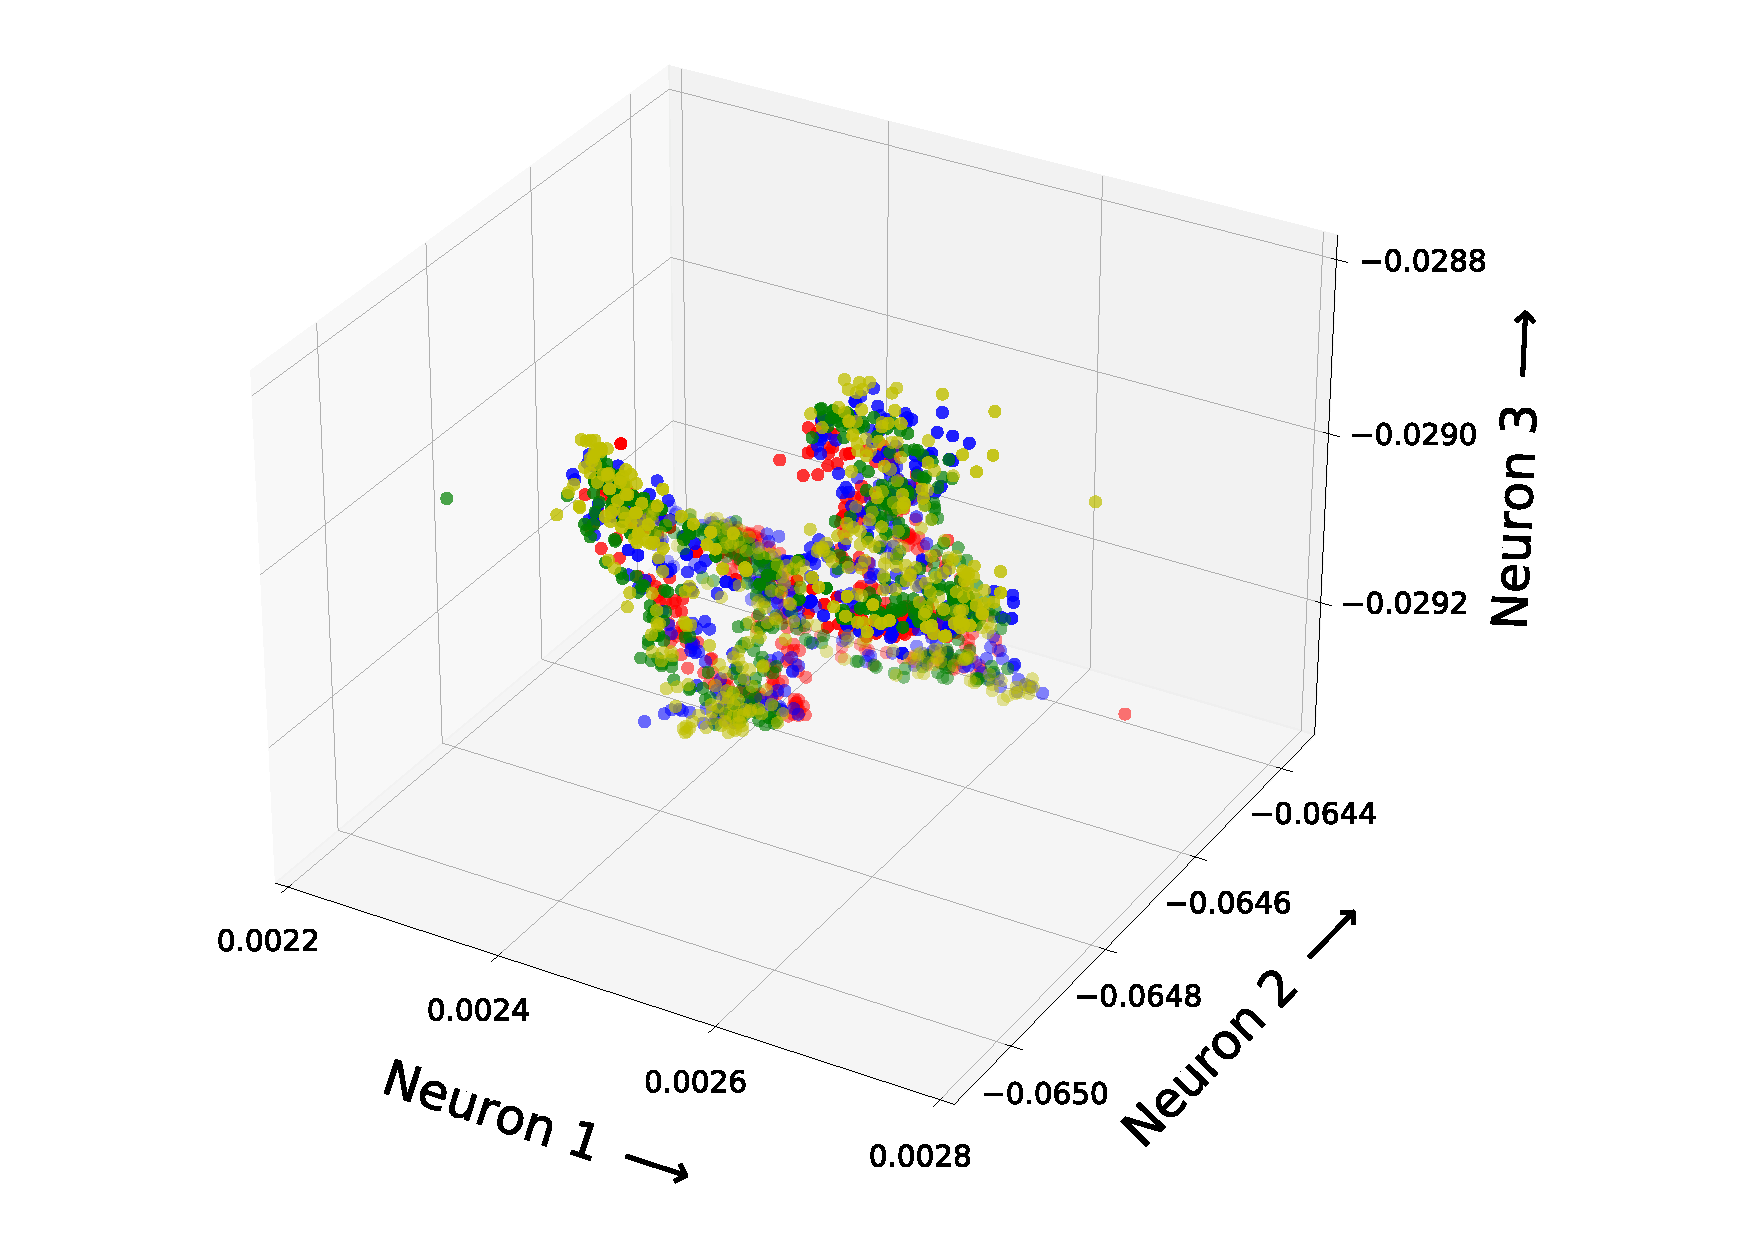
\includegraphics[width=.47\textwidth]{GAMMA_Influence_real_data/P_mech_X_data_distribution_0_GAMMA_0_0.pdf}
  \hspace{.4cm}
  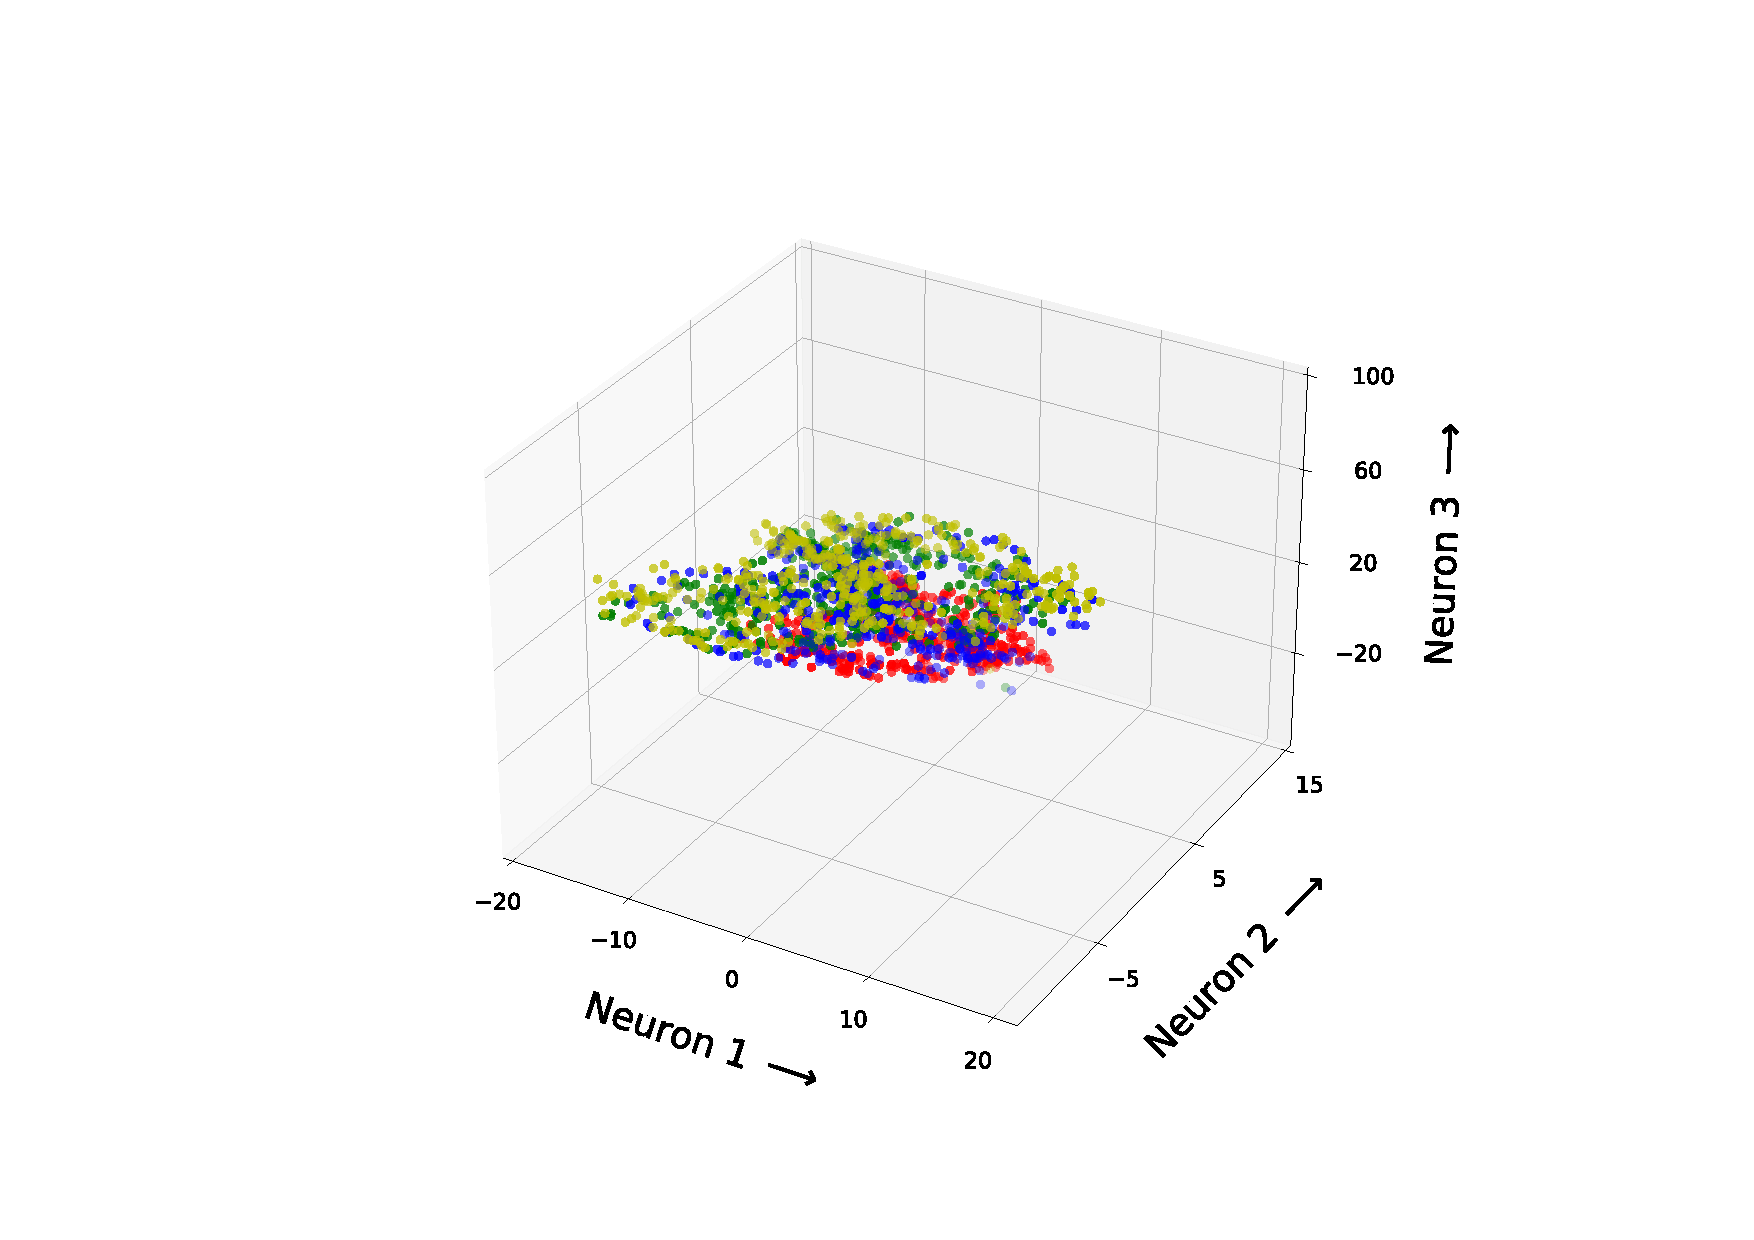
\includegraphics[width=.47\textwidth]{GAMMA_Influence_real_data/P_mech_X_data_distribution_80_GAMMA_0_0.pdf}

  \vspace{.1cm}

  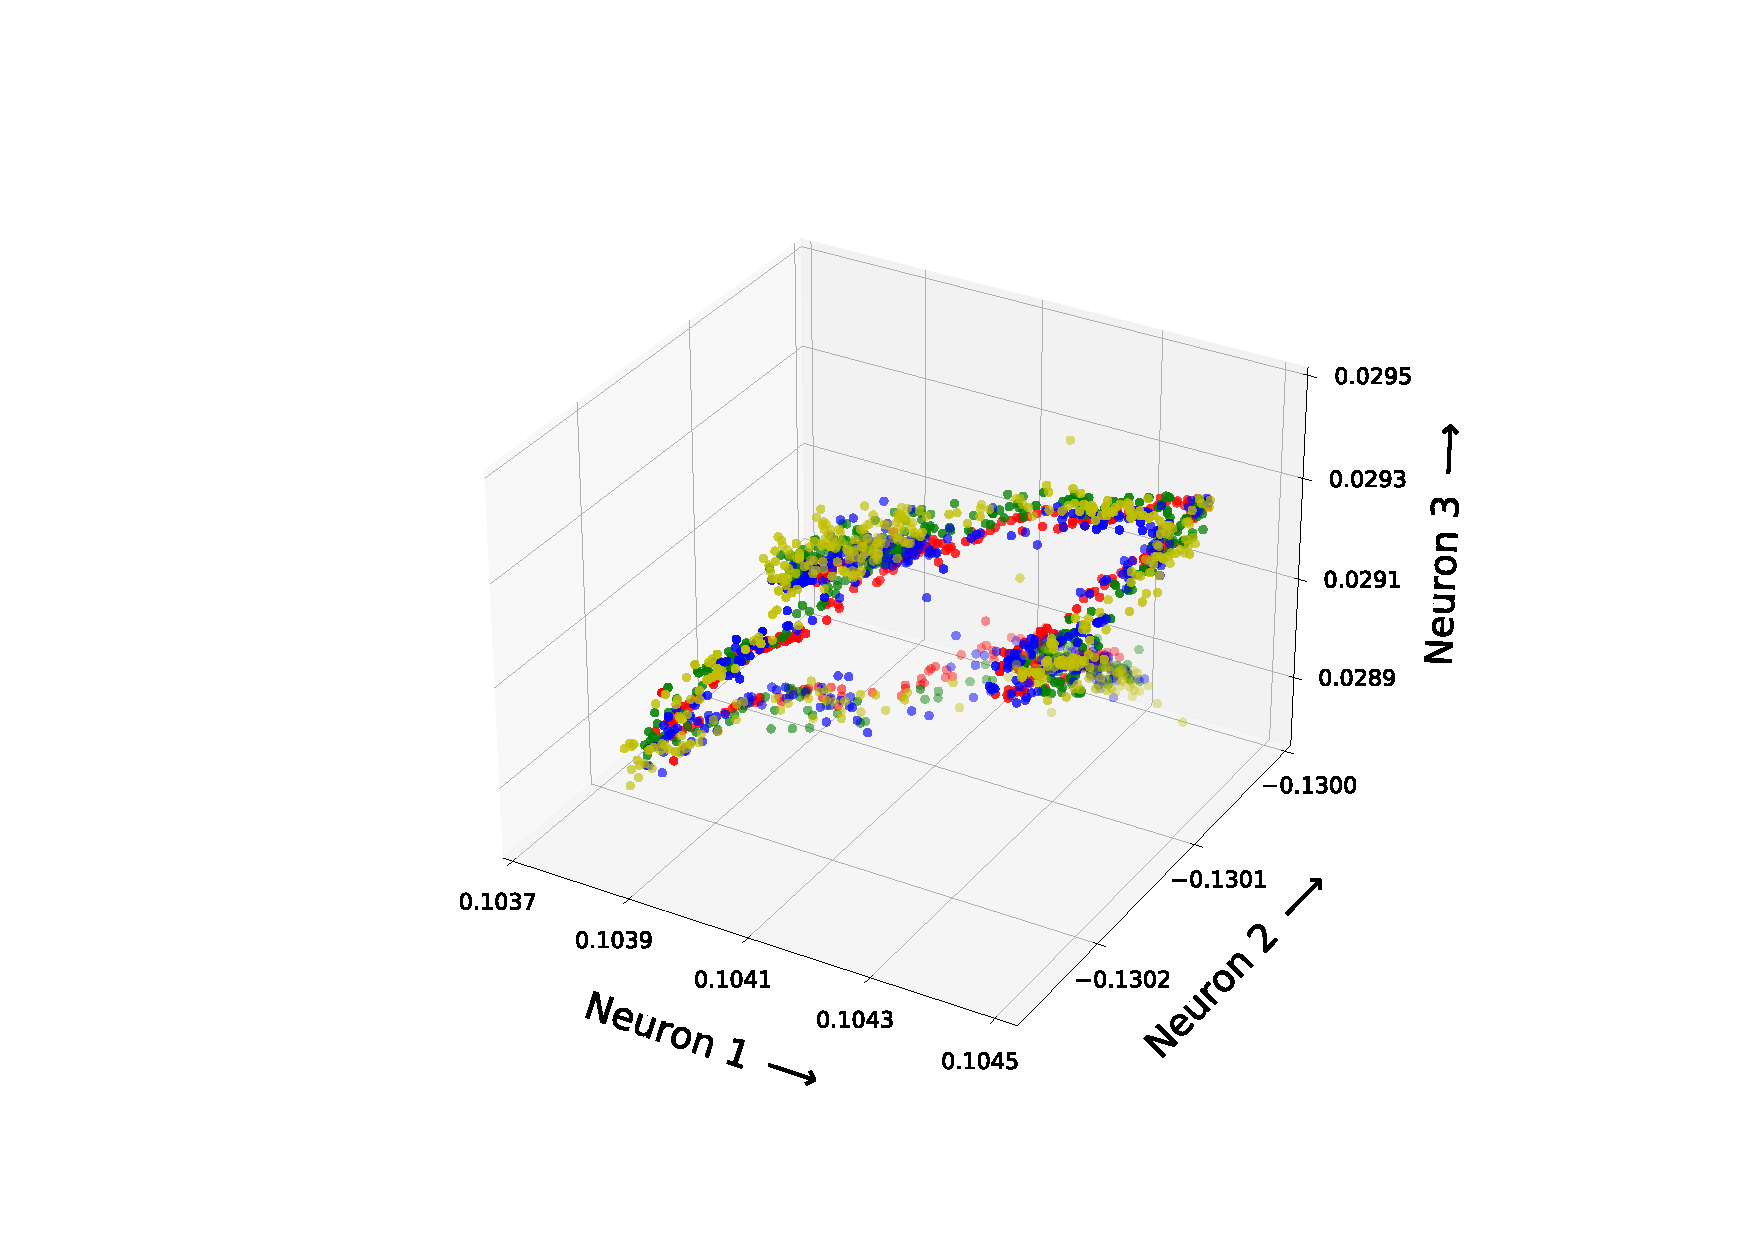
\includegraphics[width=.47\textwidth]{GAMMA_Influence_real_data/P_mech_X_data_distribution_0_GAMMA_0_05.pdf}
  \hspace{.4cm}
  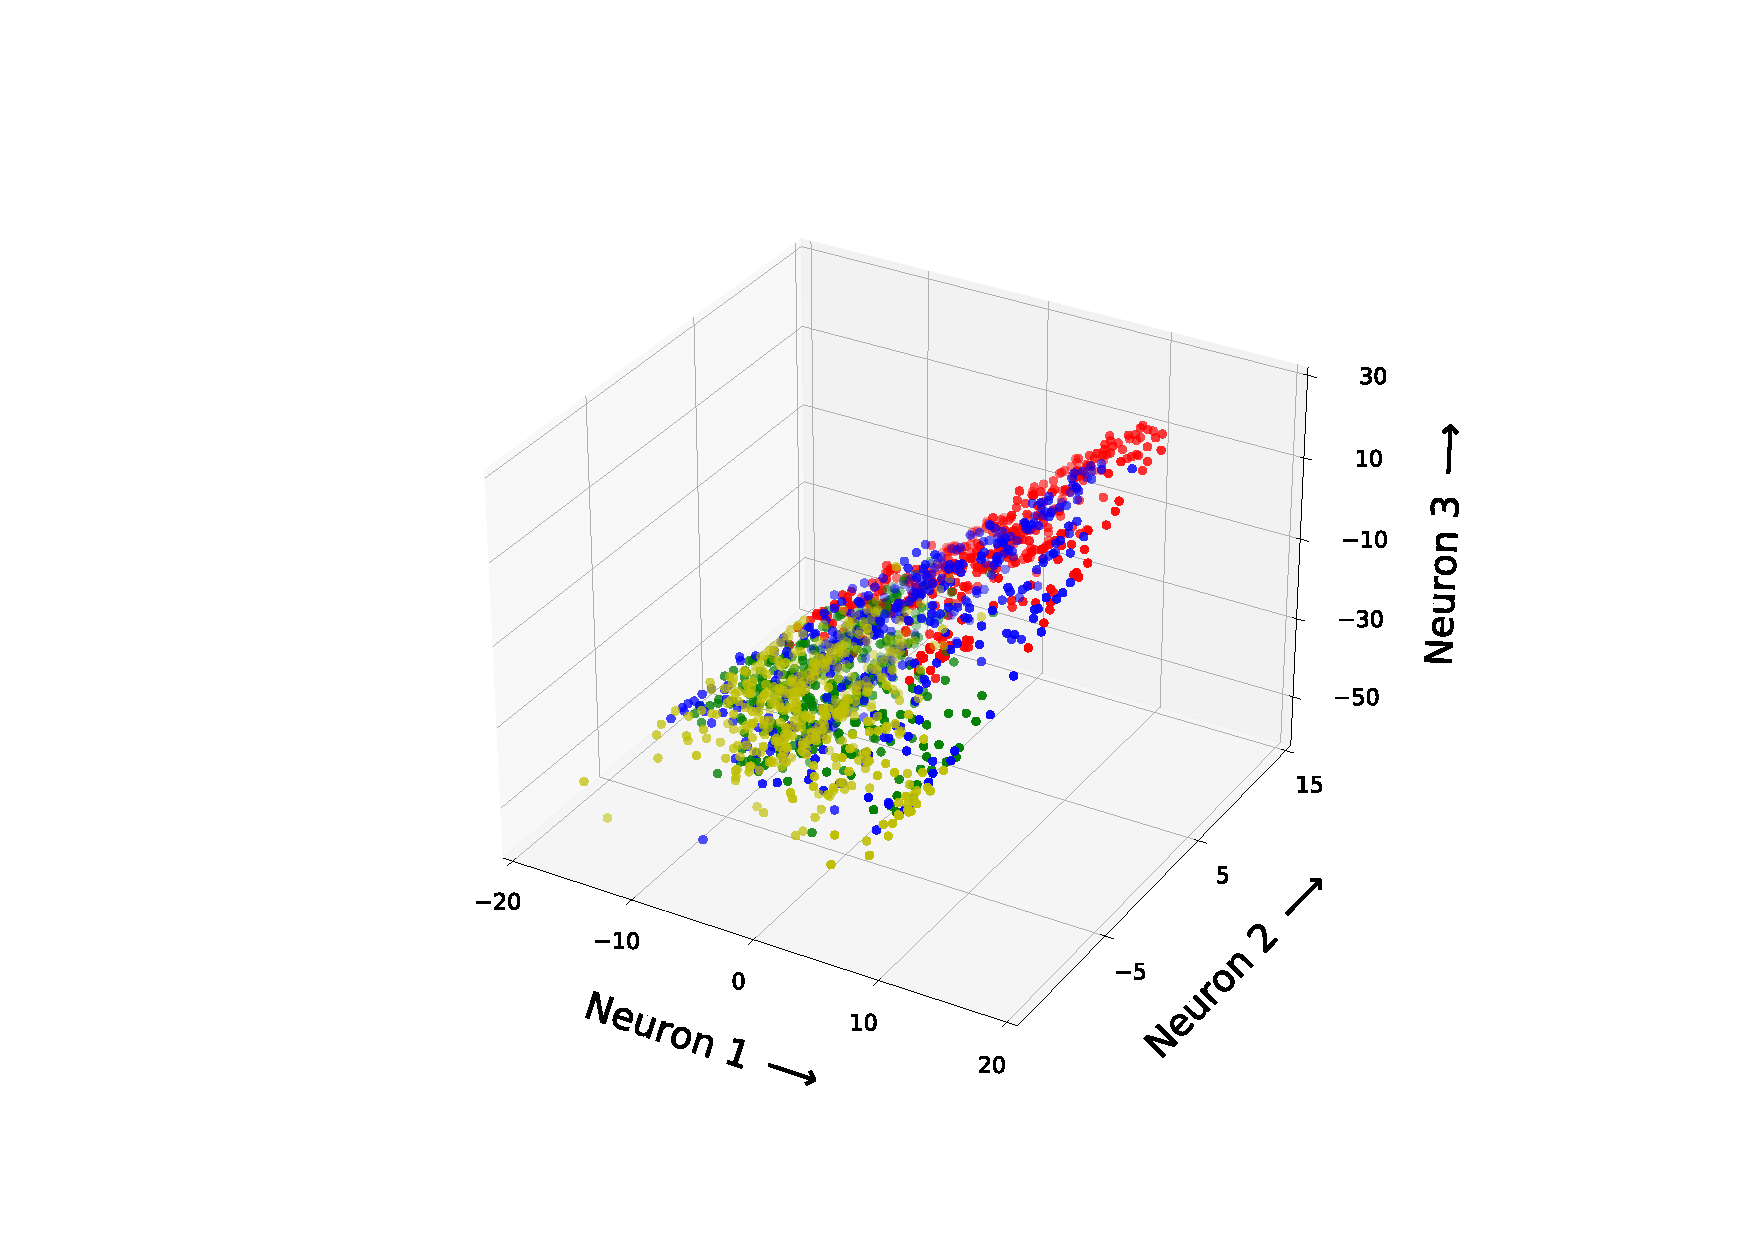
\includegraphics[width=.47\textwidth]{GAMMA_Influence_real_data/P_mech_X_data_distribution_80_GAMMA_0_05.pdf}

  \vspace{.1cm}

  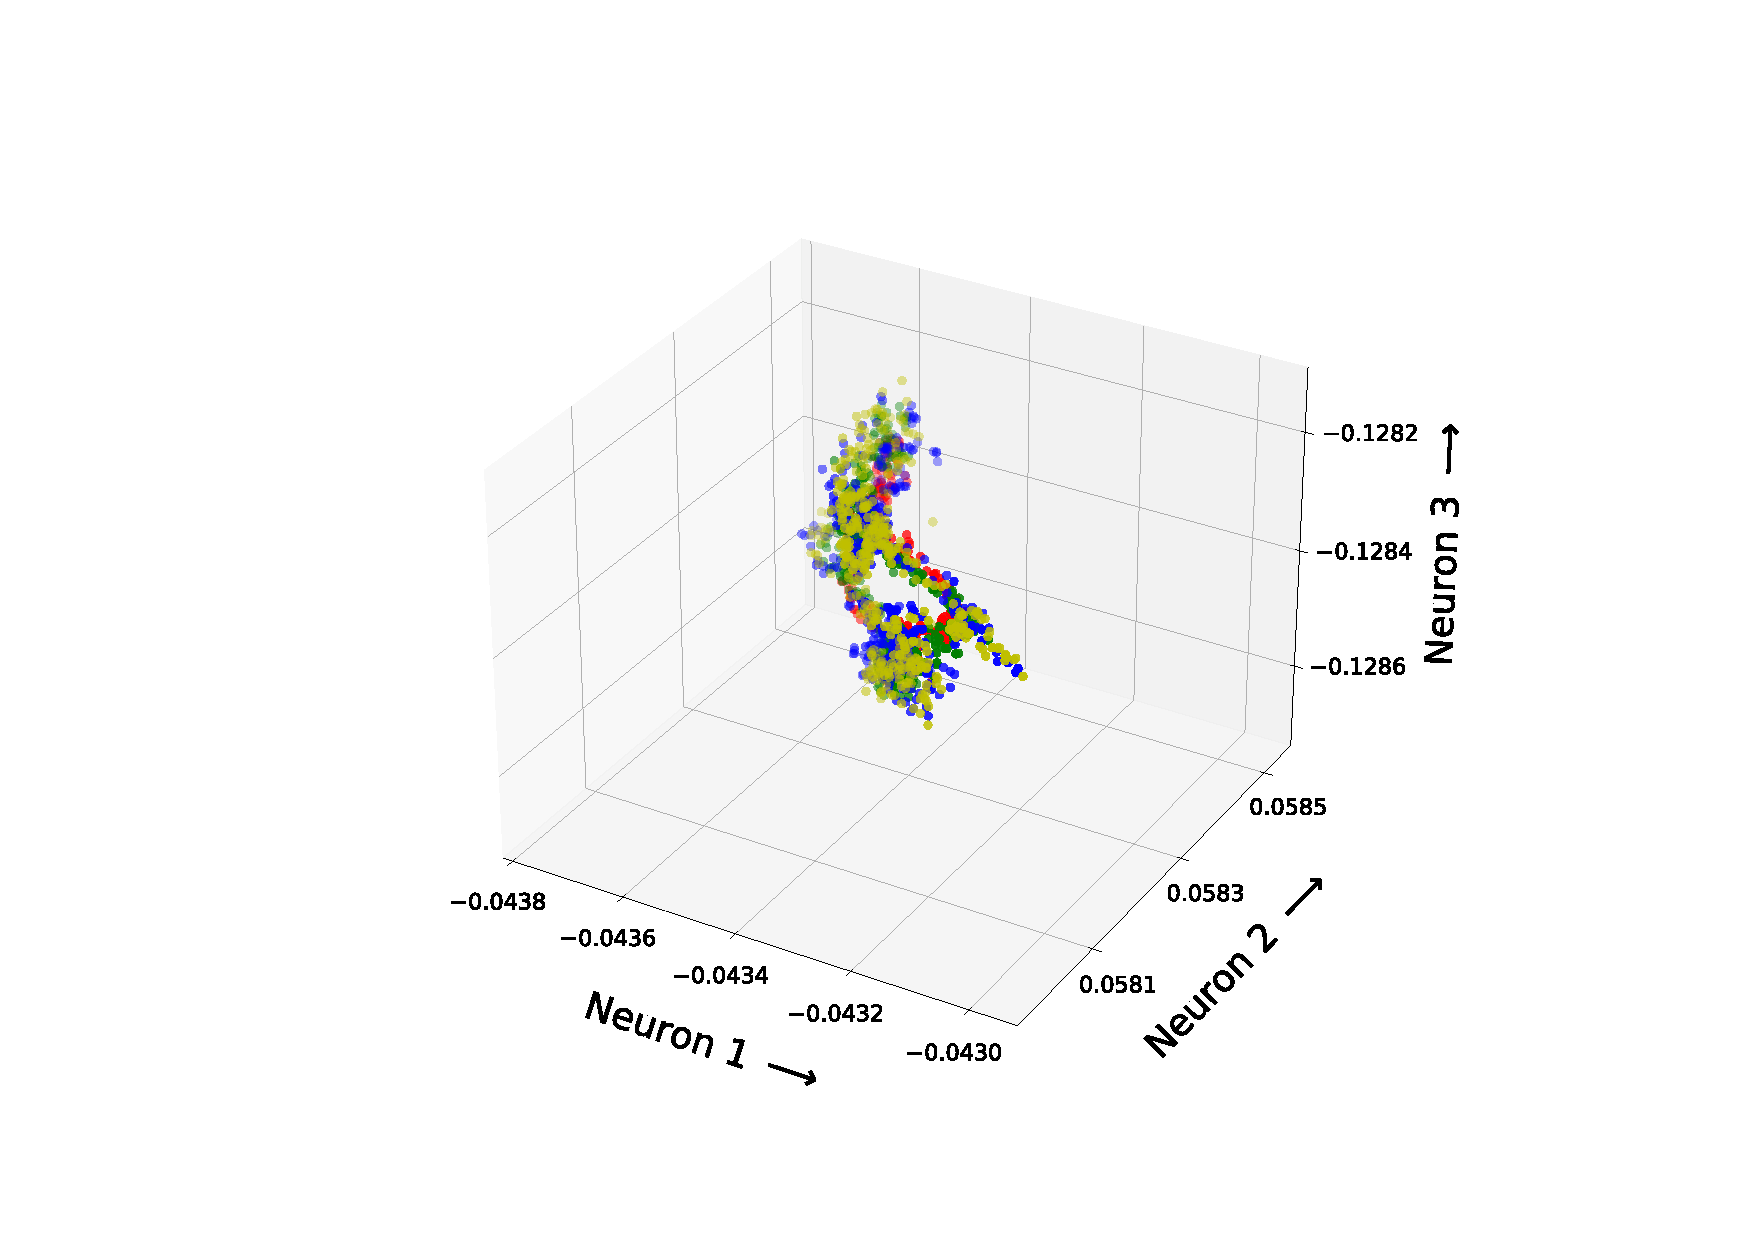
\includegraphics[width=.47\textwidth]{GAMMA_Influence_real_data/P_mech_X_data_distribution_0_GAMMA_1_0.pdf}
  \hspace{.4cm}
  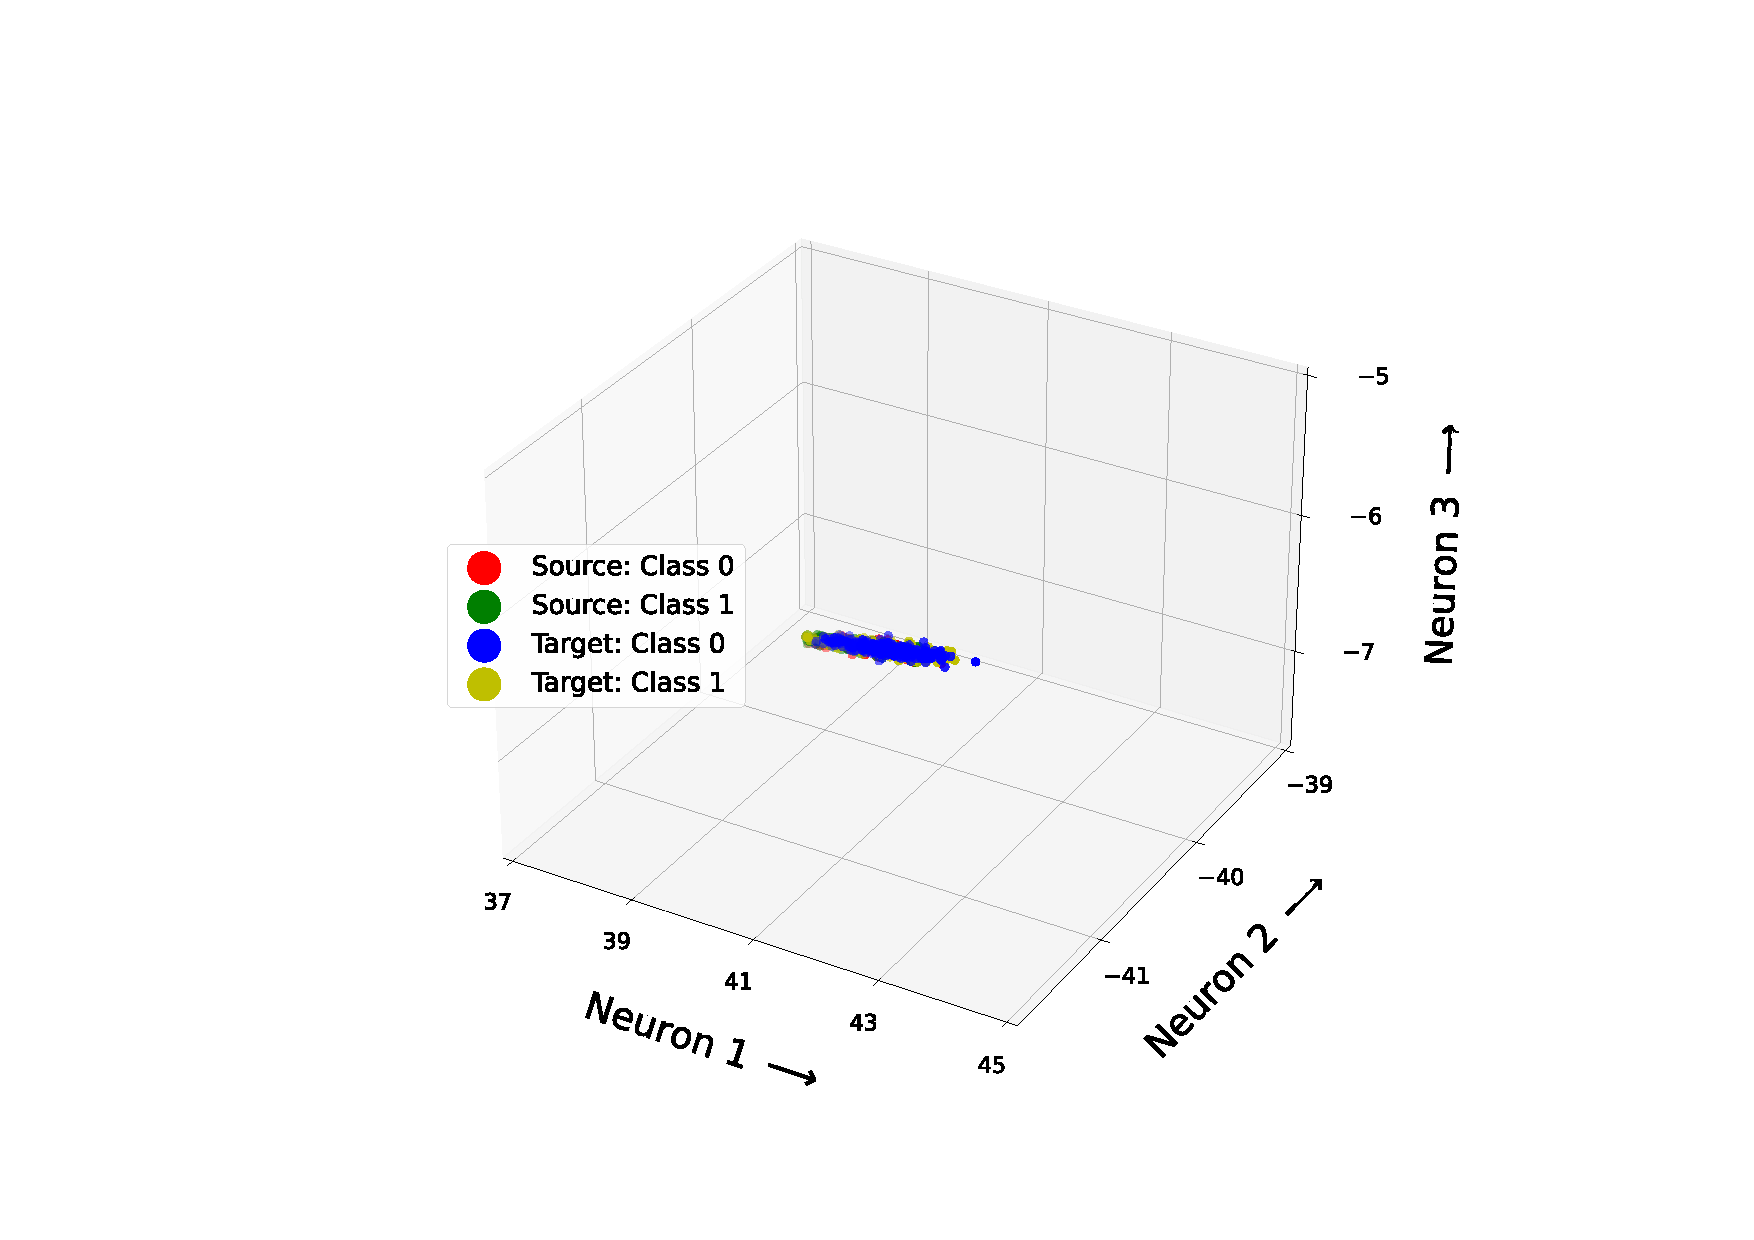
\includegraphics[width=.47\textwidth]{GAMMA_Influence_real_data/P_mech_X_data_distribution_80_GAMMA_1_0.pdf}

  \vspace{.1cm}

  \caption{Data  distribution:  Influence  of  GAMMA  on  Training with D:P\_mech./X:  GAMMA  =  0  (top),GAMMA = 0.05 (middle), GAMMA = 1 (bottom)}
  \label{fig:distribution_GAMMA_influence_real_data}
\end{figure}





\subsection{Influence of Latent Feature Space Choice on the PHM Performance}\label{ch:Influence_Layer_real_dataset}
This section analyses the effects of different MMD latent feature space choices on the model training. CNN MMD, FC MMD and FULL MMD model, which are defined as described in table \ref{tab:MMD_layer_choice}, were compared with each other. All models were trained with the D:I soll/X signal and a MMD-loss with GAMMA of 1. The experiments were repeated five times. Fig \ref{fig:target_accuracy_MMD_layer} shows the target accuracy learning curves for those experiments. When the MMD-loss is just applied in the FC layers, the training collapses in two of the five experiments (row 3 $\&$ 5). In the other three cases the accuracy has the tendency to decrease during the training. Usually the final model is picked in the end of the training. When the model's performance decreases throughout the training, one does not pick the best possible model. Compared to the FULL MMD model the CNN MMD model shows lower reproducibility in the training curves. In some of the CNN MMD experiments the target accuracy is increasing and in some decreasing during the training. Besides that, the fluctuations on the validation data cannot really be reduced throughout the training. The FULL MMD model training seems to be more stable. The fluctuations on the validation data are controlled a little bit better . Besides that, the learning curves show a higher reproducibility.  



\begin{figure}[htp]
  \centering

  \includegraphics[width=.32\textwidth]{MMD_LAYER_influence_real_data/CNN_MMD/Accuracy_Target_Domain_1.pdf}
  \hspace{.1cm}
  \includegraphics[width=.32\textwidth]{MMD_LAYER_influence_real_data/FC_MMD/Accuracy_Target_Domain_1.pdf}
  \hspace{.1cm}
  \includegraphics[width=.32\textwidth]{MMD_LAYER_influence_real_data/FULL_MMD/Accuracy_Target_Domain_1.pdf}

  \vspace{.3cm}

  \includegraphics[width=.32\textwidth]{MMD_LAYER_influence_real_data/CNN_MMD/Accuracy_Target_Domain_2.pdf}
  \hspace{.1cm}
  \includegraphics[width=.32\textwidth]{MMD_LAYER_influence_real_data/FC_MMD/Accuracy_Target_Domain_2.pdf}
  \hspace{.1cm}
  \includegraphics[width=.32\textwidth]{MMD_LAYER_influence_real_data/FULL_MMD/Accuracy_Target_Domain_2.pdf}

  \vspace{.3cm}

  \includegraphics[width=.32\textwidth]{MMD_LAYER_influence_real_data/CNN_MMD/Accuracy_Target_Domain_3.pdf}
  \hspace{.1cm}
  \includegraphics[width=.32\textwidth]{MMD_LAYER_influence_real_data/FC_MMD/Accuracy_Target_Domain_3.pdf}
  \hspace{.1cm}
  \includegraphics[width=.32\textwidth]{MMD_LAYER_influence_real_data/FULL_MMD/Accuracy_Target_Domain_3.pdf}
  
    \vspace{.3cm}

  \includegraphics[width=.32\textwidth]{MMD_LAYER_influence_real_data/CNN_MMD/Accuracy_Target_Domain_4.pdf}
  \hspace{.1cm}
  \includegraphics[width=.32\textwidth]{MMD_LAYER_influence_real_data/FC_MMD/Accuracy_Target_Domain_4.pdf}
  \hspace{.1cm}
  \includegraphics[width=.32\textwidth]{MMD_LAYER_influence_real_data/FULL_MMD/Accuracy_Target_Domain_4.pdf}
  
    \vspace{.3cm}
    
  \includegraphics[width=.32\textwidth]{MMD_LAYER_influence_real_data/CNN_MMD/Accuracy_Target_Domain_5.pdf}
  \hspace{.1cm}
  \includegraphics[width=.32\textwidth]{MMD_LAYER_influence_real_data/FC_MMD/Accuracy_Target_Domain_5.pdf}
  \hspace{.1cm}
  \includegraphics[width=.32\textwidth]{MMD_LAYER_influence_real_data/FULL_MMD/Accuracy_Target_Domain_5.pdf}


  \caption{Target Accuracy: Influence of MMD layer Choice on Training: CNN MMD (left), FC MMD (middle), FULL MMD (right)}
  \label{fig:target_accuracy_MMD_layer}
\end{figure}


\subsection{PHM Performance}\label{ch:PHM_performance}

In this chapter the utility and applicability of the presented approach on a real world task is evaluated by the target accuracy on the test data. During the training process the model with the highest balanced target accuracy on the validation data was picked to compare the approaches. In a first step, the model performance on all of the 49 signals was evaluated without the MMD-loss. In a second step, 7 promising signals, which showed high classification accuracy, were picked. These signals were then used to evaluate FULL MMD, FC MMD and CNN MMD. Each model was optimized with different GAMMAs (0.05 $\&$ 0.5 $\&$ 1). The resulting 9 models were compared with a baseline model, which was not optimized with a MMD-loss. Table \ref{tab:Mean_Accuracy} shows the target accuracy, averaged over 5 equally executed experiments. For 4 of the 7 signals the FULL MMD and for the others the CNN MMD model performed best. The MMD-loss increased the accuracy with up to 10.18$\%$. Table \ref{tab:Variance_Accuracy} shows the target accuracy variances for all models and selected signals. The best performing model usually shows low to average variances. A low variance verifies a high degree of reproducibility in the repeated experiments, which demonstrates the meaningfulness of the results. This proves the applicability and utility of a MMD-loss for reducing the domain discrepancy in PHM related tasks. Table \ref{tab:Average_Variance_Accuracy} shows the average variance over all 105 experiments for MMD-based models and 35 experiments for the baseline model. The FULL MMD has the lowest and the FC MMD the highest average target accuracy variance from the MMD-based models. This shows that the FULL MMD model has the highest reproducibility and the lowest fluctuation during the training. As mentioned in the results of the dummy dataset, a reason might be the contradicting training goals when evaluating the MMD as well as the source CE-loss just in the FC layers. This might lead to instabilities and a training which is more prone to getting stuck in local minima. The signals recorded during the constant and direction change excitement of the machines are especially suitable for the PHM of BSDs. 

\begin{comment}
Windowing functions split the recorded data in shorter sequences. The generated windows should capture the degradation related patterns of the vibration signals. For this reason, the windows should be adapted according to the consistency and periodicity of the data. In this thesis a window size of 1024 was chosen. The windowing requirements are different for the different machine excitements (constant speed excitement, direction change excitement and sweep excitement). The windows are too short to capture one whole period of of forward and backward motion in the data recorded during constant speed machine excitement. The data can be separated in phases of constant speed and direction change, which each contains roughly 1000 datapoints. The windows are of equal size as the described phases in the data. Since the windows are not synchronized with those phases, they overlap to a large extent but do not cover them perfectly. The windows are big enough to capture several periods of forward and backward movements in data recorded during direction change excitement. When exciting the machine with a sweep signal the PHM system should better process the whole corresponding vibration signal. It is important to capture the changing frequencies and amplitudes during the complete sweep excitement. The best PHM results were achieved on data recorded during constant speed and  direction change excitement of the machine. This shows that the windowing did not work very well on the data recorded during sweep excitement. Generally, when choosing the window size, there is a trade-off between the window size and the number of windows generated from the data. Both extremes (few big windows and numerous small windows) might lead to problems during the training. The PHM results can probably be improved by an intelligent and adaptive preprocessing to generate suitable and synchronized data windows. Azamfat et al \cite{AZAMFAR2020103932} present such an approach. They apply a constant excitement to the machine and separate the data BSD phases of constant velocity direction change movement. The PHM system just relies on the data recorded during BSD constant velocity. The signals D:I\_ist/X (actual electrical power), D:I\_soll/X (target electrical power) and D:P\_mech./X (mechanical power) coming from the controller show high potential for the PHM task. The most suitable accelerometer installation is the one on the BSD nut. Pandahare et al \cite{Pandhare2021} discovered similar results. Often in real operational scenarios such an installation is impractical \cite{Pandhare2021}. Alternatively to the BSD nut position, this thesis shows, that the top LGS achieves better PHM results than the bottom one.
\end{comment}


\begin{sidewaystable}
\begin {table}[H]
\centering
\begin{tabular}{llllllllll}
  \toprule
  Model          & GAMMA    & D:I\_ist/X & D:I\_soll/X & D:P\_mech./X & C:z\_top & C:z\_nut & D:x\_nut & D:z\_top \\
  \midrule
  
  \vspace{1cm}
  
    \thead{BASE- \\ LINE}  & -      & 70.08 & 75.62 & 74.7 & 69.14 & 57.4 & 58.74 & 57.88\\


 
                            & 0.05   & 71.56 & 75.42 & \textbf{78.96} & 72.36 & 58.10 & 49.52 & \textbf{62,64}\\
    \thead{FULL \\ MMD}     & 0.5    & 73.78 & 74.84 & 52.78 & \textbf{75.92} & \textbf{64.76} & 50.52 & 49,94\\
    
    \vspace{1cm}
    
                            & 1      & 72.98 & 75.18 & 49.80 & 74.12 & 57.02 & 50.62 & 50.52\\


                            & 0.05   & 73.60 & 76.38 & 74.98 & 71.36 & 57.48 & 52.44 & 61.3\\
    \thead{FC \\ MMD}       & 0.5    & 70.74 & 74.86 & 72.62 & 69.32 & 59.76 & 50.12 & 53.22\\
    
    \vspace{1cm}
    
                            & 1      & 73.42 & 65.46 & 76.96 & 62.34 & 58.86 & 50.92 & 53.96\\

                            & 0.05   & 71.62 & \textbf{76.44} & 51.80 & 73.20 & 59.30 & 58.04 & 53.82\\
    \thead{CNN \\ MMD}      & 0.5    & \textbf{73.90} & 75.86 & 51.58 & 72.28 & 55.76 & 68.04 & 51.72\\
                            & 1      & 73.80 & 73.82 & 51.12 & 72.18 & 54.28 & \textbf{68.92} & 51.28\\
 \addlinespace
 \hline
 \thead{MMD\\GAIN:} &  & +3.82 & +0.82 & +4.26 & +6.78 & +7.36 & +10.18 & +4.76\\
 
  \bottomrule
\end{tabular}
\caption {Mean target test accuracy (\%)} \label{tab:Mean_Accuracy} 
\end {table}
\end{sidewaystable}

\begin{sidewaystable}
\begin {table}[H]
\centering
\begin{tabular}{llllllllll}
  \toprule
  Model          & GAMMA    & D:I\_ist/X & D:I\_soll/X & D:P\_mech./X & C:z\_top & C:z\_nut & D:x\_nut & D:z\_top  \\
  \midrule

    \vspace{1cm}

    \thead{BASE- \\ LINE}   & -      & 2.07 & 0.27 & 2.20 & 2.55 & 1.11 & 1.04 & 1.22\\
 
                            & 0.05   & 1.06 & 0.74 & \textbf{1.79} & 1.80 & 2.04 & 1.39 & \textbf{2.48}\\
    \thead{FULL \\ MMD}     & 0.5    & 0.72 & 1.44 & 3.33 & \textbf{1.72} & \textbf{1.42} & 1.23 & 1.02\\
    
    \vspace{1cm}  
    
                            & 1      & 0.76 & 0.81 & 0.87 & 6.06 & 5.57 & 0.96 & 0.79\\



                            & 0.05   & 1.96 & 0.61 & 1.86 & 1.82 & 1.63 & 3.86 & 1.60\\
    \thead{FC \\ MMD}       & 0.5    & 1.34 & 0.72 & 11.06 & 6.42 & 2.28 & 0.45 & 3.14\\
    
    \vspace{1cm}
    
                            & 1      & 0.96 & 12.01 & 5.46 & 8.18 & 2.13 & 0.93 & 2.70\\
                            & 0.05   & 2.13 & \textbf{0.53} & 2.39 & 1.12 & 4.01 & 4.18 & 7.26\\
    \thead{CNN \\ MMD}      & 0.5    & \textbf{0.25} & 1.57 & 1.08 & 1.22 & 3.27 & 3.51 & 3.22\\
                            & 1      & 0.51 & 1.25 & 2.02 & 2.51 & 4.54 & \textbf{2.54} & 2.34\\
  \bottomrule
\end{tabular}
\caption {Standard deviation target test accuracy (\%)} \label{tab:Variance_Accuracy} 
\end {table}
\end{sidewaystable}


\begin {table}[H]
\centering
\begin{tabular}{lllll}
  \toprule
  Model & BASE-LINE & FULL MMD & FC MMD & CNN MMD\\
  \midrule
  AVG VARIANCE & 1.50 & 1.81 & 3.39 & 2.45\\
  \bottomrule
\end{tabular}
\caption {Average standard deviation target test accuracy (\%)} \label{tab:Average_Variance_Accuracy} 
\end {table}

